% !TeX spellcheck = en_GB
% %%% ***************** CHAPTER RESULTS ***************** %%%
\chapter{Results} \label{ch:Res}
% \textcolor{red}{\textbf{The overleaf file from the Results is here:} \\ \url{https://www.overleaf.com/15070250fhqztvnygzmn}} 
% \\V
%
In this chapter the results of the optimal estimation retrieval and the regional mesoscale forecast model are presented. On the basis of the methodology described in \Cref{ch:Methods} it should be evaluated if a regional mesoscale forecast model prognoses the same snowfall amount as observed with the ground based remote sensing at Haukeliseter. All days of the seven day event showed their own significances. Since some patterns repeated during these days the most interesting days, \SIlist{21;24;25}{\dec}, are picked and studied in the end of this chapter.
%ensemble member \numlist{0;1} every hour; ensemble member \numrange{2}{10} every three hours. \\
%
%\begin{itemize}
% \item \SI{21}{\dec} has convective storm from \SIrange{9}{13}{\UTC} then pulsing
% \item on \SI{23}{\dec} convective storm from \SIrange{16}{00}{\UTC} 
% \item connection with wind \Cref{fig:wind21,fig:wind22,fig:wind23,fig:wind24,fig:wind25,fig:wind26}% when pulsing event then wind observations from N\-W to S\-W
% %\item $\rightarrow$ when wind from S\-S\-W to S\-E then convective storm habit
% \item \textbf{pick interesting days:}
% 	\begin{itemize}
% 	\item \SI{21}{\dec}, because change from convective storm to pulsing event $\rightarrow$ put in the connection with wind. MEPS does catch convective part, but not as strong. High SWC$_\textit{MEPS}$ at \SI{20}{\UTC}
% %    \item \SI{22}{\dec}, because SWC$_\mathit{RETRIEVAL}$ almost same as SWC$_\mathit{MEPS}$, only \SI{2}{\hour} shift
%     \item \SI{24}{\dec}, because SWC$_\mathit{MEPS}$ almost as pulsing as SWC$_\mathit{RETRIEVAL}$ just not as strong. Also overestimation of surface snowfall from MEPS \Cref{fig:sfc_acc24}. All 10 ensemble members have pulsing. Most intense in pulsing events: control, EM1, EM4, EM5, EM7 (not shown).
% %    \item \SI{25}{\dec}, because MEPS covers the LWC at the same time as retrieval, but the retrieval does not see the snow above $\rightarrow$ weakness of retrieval is shown even though weak. See: \Cref{fig:SWC25} and \ref{fig:LWC25}. Also it has the overestimation at the surface \Cref{fig:sfc_acc25}
%     \item \SI{26}{\dec} almost correct forecasted peak, all three systems recognise stop of precipitation (retrieval a little earlier), MEPS overestimates after 12h forecast, MEPS has stronger SWP values than retrieval, no relation between wind and scatter
% 	\end{itemize}
% \item \textbf{Research question:}  \\ Does a regional mesoscale model catch the same snowfall amount as observed at a certain location?
% \end{itemize}

%%%%%%%%%%%%%%%%%%%%%%%%%%%%%%%%%%%%%%%%%%%%%%%%%%%%%%%%%%%%%%%%%%%%%%%%%%
%%% table SWP and LWP max %%%%%%%%%%%%%%%%%%%%%%%%%%%%%%%%%%%%%
%% !TeX spellcheck = en_GB
\begin{table}[h!]
	\begin{center}
		\caption{Maximum values of the snow water content and snow water path from the retrieval and MEPS}\label{tab:max_val}
		\begin{tabular}{ll|c|c|c||c|c} 
			\hline \hline
			& & \textbf{SWC}  & \textbf{HEIGHT}  & \textbf{TIME} & \textbf{SWP}    & \textbf{TIME}  \\
			& & [\SI{}{\kg\per\cubic\meter}] & [\SI{}{\meter}] &  & [\SI{}{\kg\per\square\metre}] & [\SI{}{\meter}]    \\
			\hline \hline
			\multicolumn{7}{c}{\textbf{Wed, 21 Dec 2016}} \\ \hline
			\multicolumn{2}{l|}{RETRIEVAL} & 1.08 & 600.0 & \SI{16}{\UTC} & \num{2162.2} & \SI{16}{\UTC} \\
			\multicolumn{2}{l|}{MEPS} &  &  & & &  \\
			& ensemble mean & \num{1.24} & \num{1400.0} & \SI{20}{\UTC} & \num{2833.1} &  \SI{20}{\UTC}\\
			& control & \num{2.11} & \num{1400.0} & \SI{20}{\UTC} & \num{4822.3} & \SI{20}{\UTC}\\ \hline \hline
			%              \multicolumn{8}{c}{\textbf{Thu, 22 Dec 2016}} \\ \hline
			%              \multicolumn{2}{l|}{RETRIEVAL} & \num{1.46} & \num{1200.0} & \SI{10}{\UTC} & & & \\
			%              \multicolumn{2}{l|}{MEPS} &  &  & & & & \\
			%              & ensemble mean & \num{0.99} & \num{1400.0} & \SI{14}{\UTC} & \num{0.10} & \num{2000.0} & 0\SI{02}{\UTC} \\ 
			% 			 & control & \num{1.35} & \num{1400.0} & \SI{12}{\UTC} & \num{0.20} & \num{2000.0} & 0\SI{02}{\UTC} \\ \hline \hline
			%              \multicolumn{8}{c}{\textbf{Fri, 23 Dec 2016}} \\ \hline
			% 			 \multicolumn{2}{l|}{RETRIEVAL} & \num{0.91} & \num{600.0} & \SI{23}{\UTC} & & & \\
			%              \multicolumn{2}{l|}{MEPS} &  &  & & & & \\
			%              & ensembel mean & \num{0.54} & \num{400.0} & \SI{20}{\UTC} & \num{0.10} & \num{1000.0} & \SI{15}{\UTC} \\
			%              & control & \num{0.54} & \num{400.0} & \SI{20}{\UTC} & \num{0.14} & \num{1000.0} & \SI{15}{\UTC} \\ \hline \hline
			\multicolumn{7}{c}{\textbf{Sat, 24 Dec 2016}} \\ \hline
			\multicolumn{2}{l|}{RETRIEVAL} & \num{1.39} & \num{1000.0} & 0\SI{06}{\UTC} & \num{3044.4} &  0\SI{06}{\UTC}\\
			\multicolumn{2}{l|}{MEPS} &  &  & & &  \\
			& ensemble mean & \num{0.51} & \num{800.0} & 0\SI{02}{\UTC} & \num{1087.3} &  \SI{17}{\UTC} \\
			& control & \num{0.73} & \num{1400.0} & \SI{17}{\UTC} & \num{1623.0} &  0\SI{7}{\UTC} \\ \hline \hline
			%              \multicolumn{8}{c}{\textbf{Sun, 25 Dec 2016}} \\ \hline
			% 			 \multicolumn{2}{l|}{RETRIEVAL} & \num{0.69} & \num{1400.0} & \SI{21}{\UTC} & & & \\
			%              & ensembel mean & \num{0.44} & \num{400.0} & \SI{20}{\UTC} & \num{0.32} & \num{200.0} & \SI{17}{\UTC} \\
			% 			 & control & \num{0.50} & \num{800.0} & \SI{20}{\UTC} & \num{0.34} & \num{200.0} & \SI{17}{\UTC} \\ \hline \hline
			\multicolumn{7}{c}{\textbf{Mon, 26 Dec 2016}} \\ \hline
			\multicolumn{2}{l|}{RETRIEVAL} & \num{1.25} & \num{600.0} & \SI{15}{\UTC} & \num{1689.1} & \SI{15}{\UTC} \\
			& ensembel mean & \num{0.95} & \num{800.0} & \SI{16}{\UTC} & \num{2237.0} & \SI{16}{\UTC} \\
			& control & \num{1.55} & \num{1000.0} & \SI{11}{\UTC} & \num{3414.9} & \SI{17}{\UTC} \\ \hline \hline
			%              \multicolumn{8}{c}{\textbf{Tue, 27 Dec 2016}} \\ \hline
			%              \multicolumn{2}{l|}{RETRIEVAL} & -- & -- & -- & & & \\
			%              & ensembel mean & \num{0.16} & \num{400.0} & 0\SI{00}{\UTC} & \num{0.13} & \num{800.0} & \SI{23}{\UTC} \\
			%              & control & \num{0.16} & \num{400.0} & 0\SI{00}{\UTC} & \num{0.25} & \num{800.0} & \SI{23}{\UTC} \\ \hline \hline
		\end{tabular}
	\end{center}
\end{table}
%%%%%%%%%%%%%%%%%%%%%%%%%%%%%%%%%%%%%%%%%%%%%%%%%%%%%%%%%%%%%%%%%%%%%%%%%%

%%%%%%%%%%%%%%%%%%%%%%%%%%%%%%%%%%%%%%%%%%%%%%%%%%%%%%%%%%%%%%%%%%%%%%%%%%
%%%%%%%%% SFC ACCUMULATION %%%%%%%%%%%%%%
% !TeX spellcheck = en_GB
\section{Surface snowfall accumulation}
The surface accumulation is a good point to start to see, if the retrieved snowfall amounts at the surface catch the boundary condition as of the double fence. Precipitation amount at the surface are shown in \Cref{fig:sfc_acc}. The figures are representing the observed surface precipitation accumulation in \SI{}{\mm} over \SI{48}{\hour}. Accumulation, measured by the double fence are presented as purple hexagons. Minutely retrieved surface snowfall amount in dash-dotted orange. The ten \SI{48}{\hour} forecast ensemble members are lines in black and grey, the deterministic and its perturbed ensemble members, respectively. The blue dashed line shows the ensemble mean of all ten members. Since the deterministic and the first ensemble member are having values every hour and the other perturbed members only every three hours, shows the ensemble mean the precipitation amount at 0\SI{0}{\hour}, \SI{3}{\hour}, $\ldots$, \SI{21}{\hour}, \SI{24}{\hour}, $\ldots$, \SI{48}{\hour} forecast time. 
Underneath is the associated \SI{10}{\minute} average wind of the last hour from the \SI{10}{\metre} weather mast at Haukeliseter, to see if surface accumulation observations are influenced by wind. 
%%% image surface accumulation %%%%%%%%%%%%%%%%%%%%%%%%%%%%%%%%%%%%%
% !TeX spellcheck = en_GB
%\begin{landscape}
\begin{figure}[t!]
	\centering
	% 21/12
	\begin{subfigure}[t]{0.49\textwidth}		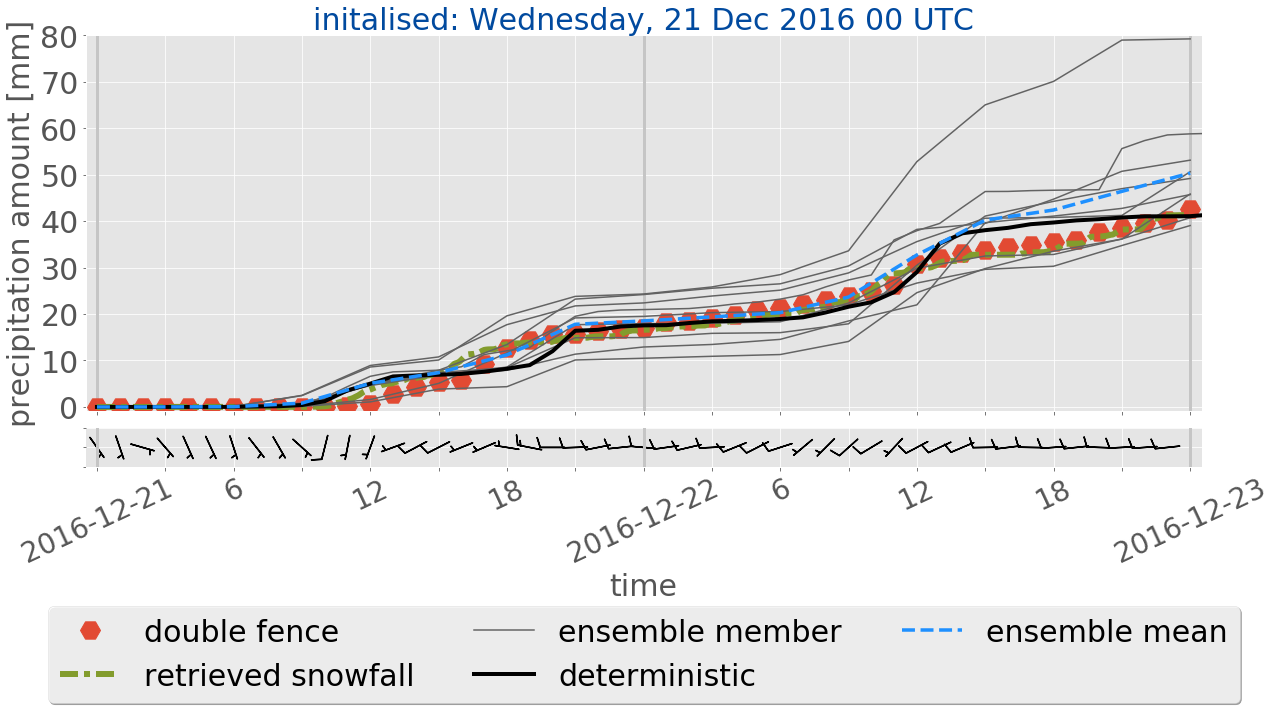
\includegraphics[trim={3.cm 2.6cm 2.cm 1.9cm},clip,width=\textwidth]{./fig_sfc_acc/acc_wind_20161221_00}
		\caption{}\label{fig:sfc_acc21}
	\end{subfigure}
	% 22/12
	\begin{subfigure}[t]{0.49\textwidth}		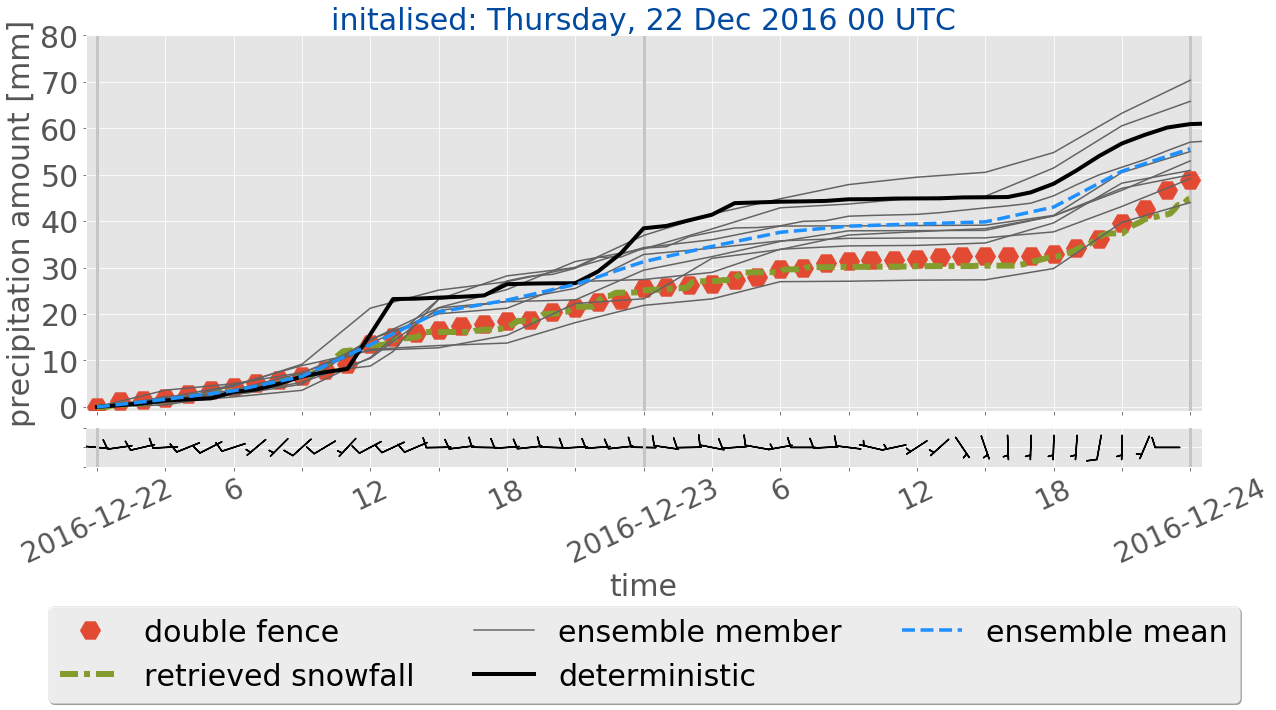
\includegraphics[trim={3.cm 2.6cm 2.cm 1.9cm},clip,width=\textwidth]{./fig_sfc_acc/acc_wind_20161222_00}
		\caption{}\label{fig:sfc_acc22}
	\end{subfigure}
	%	\end{figure}
	%   \begin{figure}\ContinuedFloat
	% 23/12
	\begin{subfigure}[t]{0.49\textwidth}	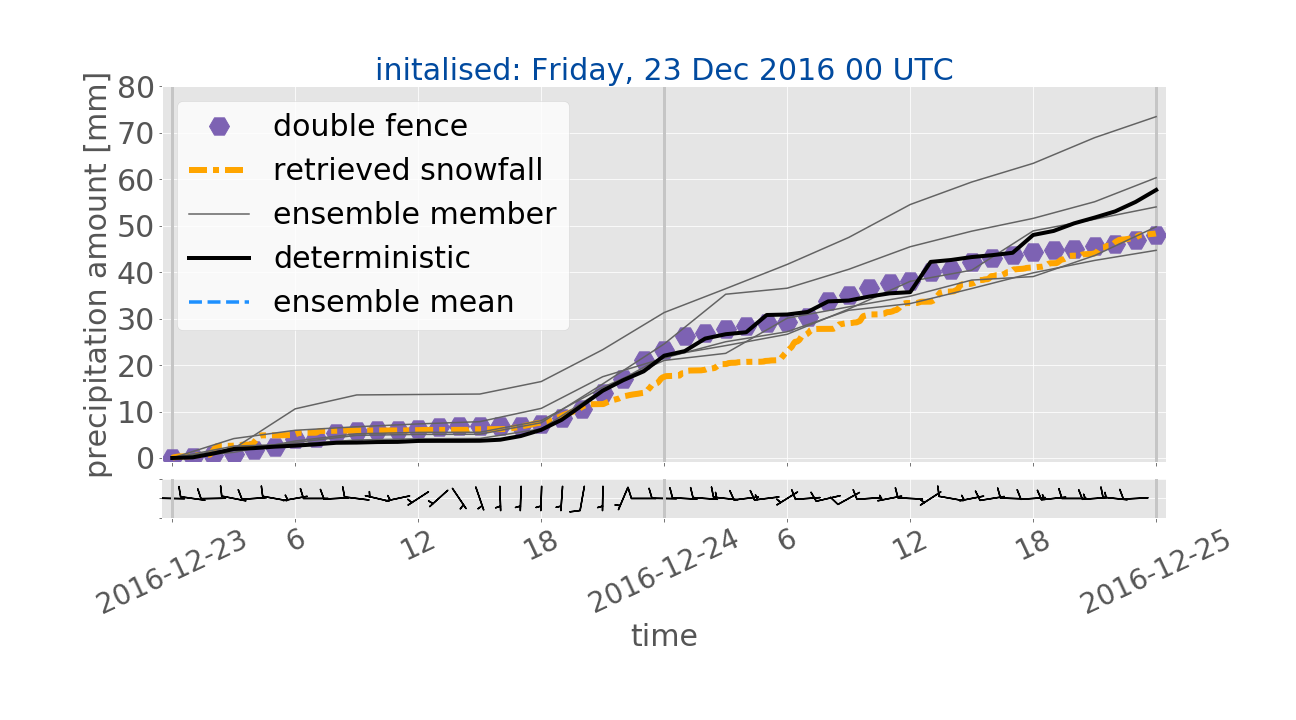
\includegraphics[trim={3.cm 2.6cm 2.cm 1.9cm},clip,width=\textwidth]{./fig_sfc_acc/acc_wind_20161223_00}
		\caption{}\label{fig:sfc_acc23}
	\end{subfigure}
	% 24/12
	\begin{subfigure}[t]{0.49\textwidth}			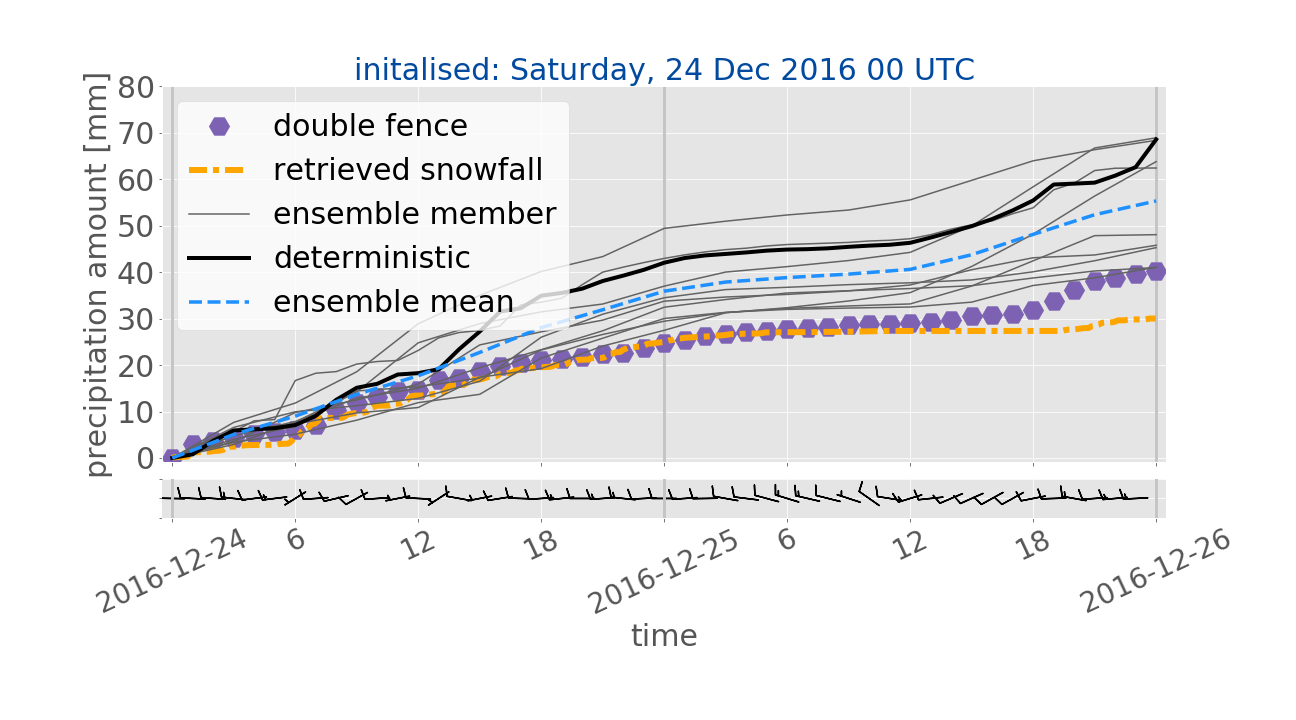
\includegraphics[trim={3.cm 2.6cm 2.cm 1.9cm},clip,width=\textwidth]{./fig_sfc_acc/acc_wind_20161224_00}
		\caption{}\label{fig:sfc_acc24}
	\end{subfigure}
	% 25/12
	\begin{subfigure}[t]{0.49\textwidth}
		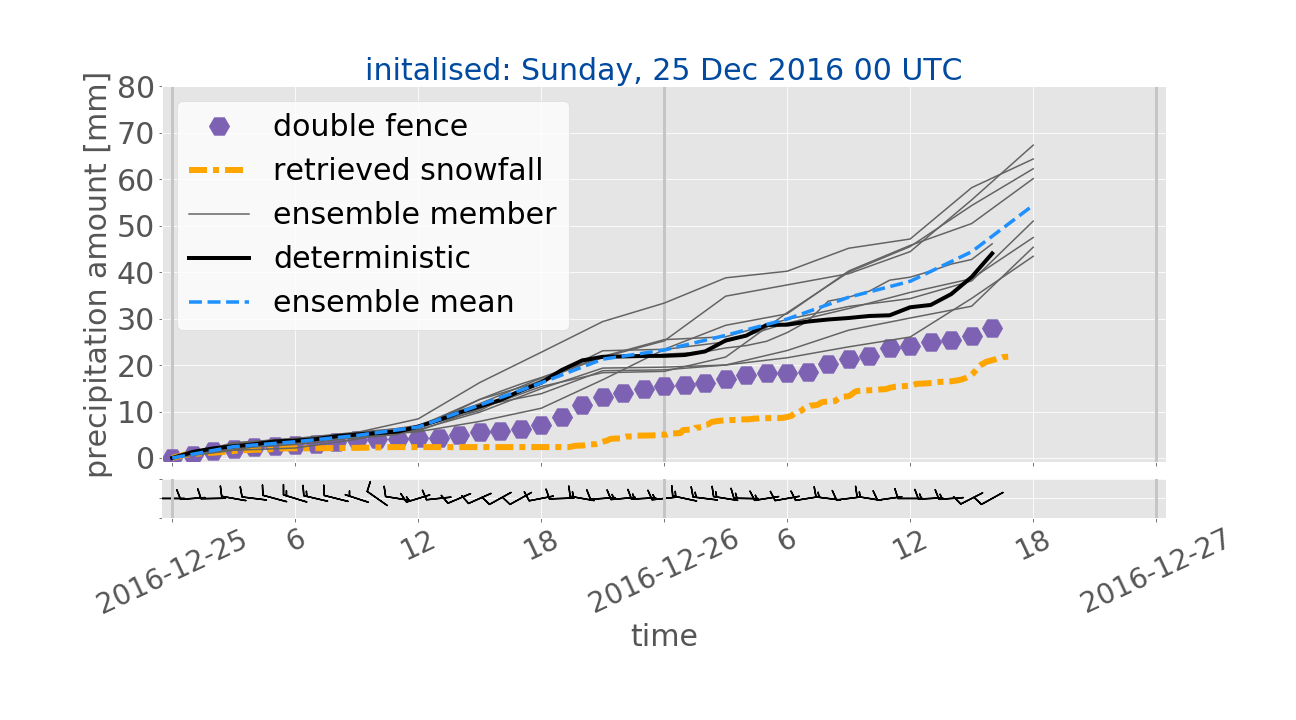
\includegraphics[trim={3.cm 2.6cm 2.cm 1.9cm},clip,width=\textwidth]{./fig_sfc_acc/acc_wind_20161225_00}
		\caption{}\label{fig:sfc_acc25}
	\end{subfigure}
	% 26/12
	\begin{subfigure}[t]{0.49\textwidth}	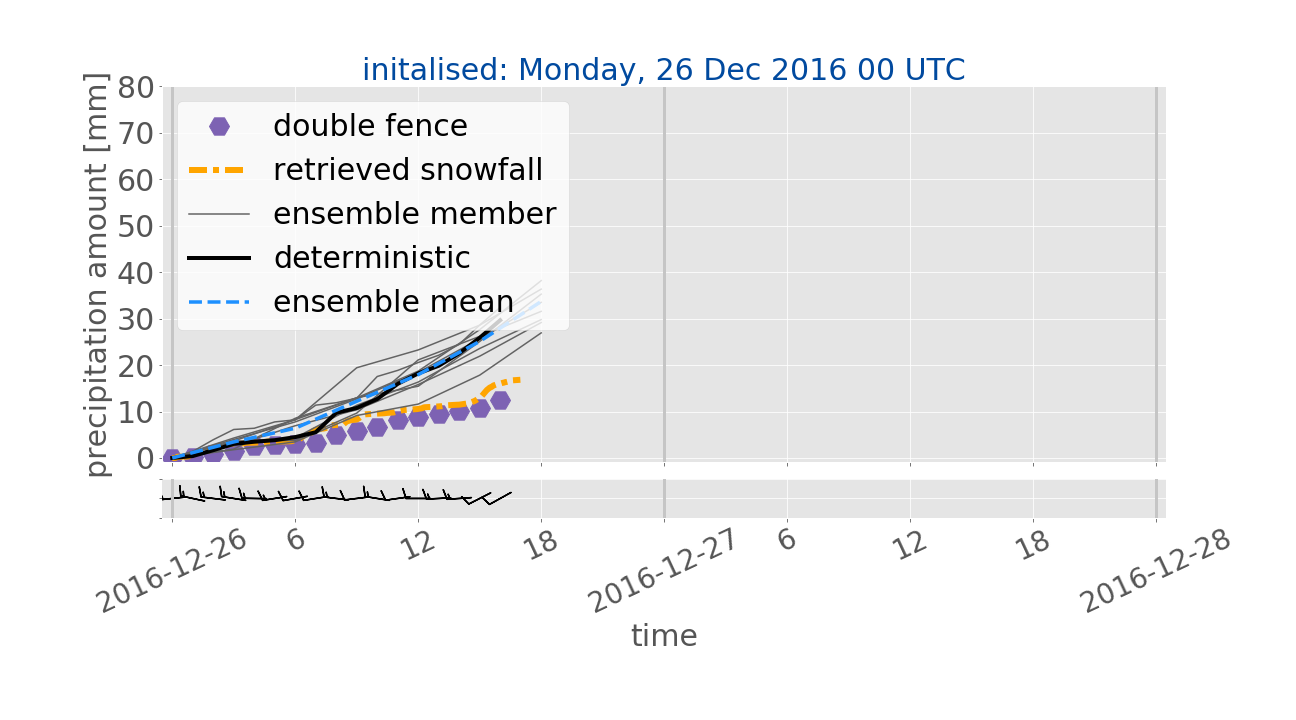
\includegraphics[trim={3.cm 2.6cm 2.cm 1.9cm},clip,width=\textwidth]{./fig_sfc_acc/acc_wind_20161226_00}
		\caption{}\label{fig:sfc_acc26}
	\end{subfigure}
	\caption{Surface snowfall accumulation. Representing the values from the double fence in purple, hexagons; optimal estimation retrieval output at snow layer height \SI{800}{\metre} in dash-dotted orange; and ensemble member deterministic forecast, initialised at 0\SI{00}{\UTC} in black and its nine perturbed ensemble members in grey. The ensemble mean of all ten members is shown in blue dashed.  Underneath are the associated last \SI{10}{\minute} average wind from the weather mast at \SI{10}{\metre} height. }\label{fig:sfc_acc}
\end{figure}



%%%%%%%%%%%%%%%%%%%%%%%%%%%%%%%%%%%%%%%%%%%%%%%%%%%%%%%%%%%%%%%%%%%%%%%%%%
\noindent
In general show the \SI{48}{\hour} surface accumulation in \Cref{fig:sfc_acc21,fig:sfc_acc22,fig:sfc_acc23} a good agreement between the foretasted values and the retrieved snowfall amount when comparing to the double fence. \SI{24}{\dec} and \SI{25}{\dec} show a disagreement between the surface observations and the model forecast. During this days is the precipitation amount predicted by MEPS for all ten ensemble members higher than for the measured accumulation. The possible reason for the overestimation at the ground is later discussed in \Cref{sec:2412:surface} and \ref{sec:2512:surface}. \\
Retrieved accumulation almost always reached the boundary condition of the double fence observations. The only well pronounced mismatch is seen on \SI{25}{\dec}, where it measures much less than the double fence gauge.  
\\ \\
The surface accumulation initialised on the \SI{21}{\dec} at 0\SI{0}{\UTC} has one ensemble member overestimating the precipitation amount after \SI{33}{\hour} forecast time. Otherwise, agree all three systems well with each other and the perturbed ensemble members are equally spread around the deterministic forecast.
\\
On \SI{22}{\dec} (\Cref{fig:sfc_acc22}) fit the ensemble mean relatively well to the observed surface accumulation, were the double fence estimates the least amount. Clearly, the ensemble members in grey are not equally distributed around the deterministic forecast. The deterministic is predicting more surface accumulation with a large jump after \SI{11}{\hour}, always being higher than most of the ensemble members and observations. 
\\
When too few ensemble members were present, like on \SI{23}{\dec}, no ensemble mean is calculated. \Cref{fig:sfc_acc23} shows a good agreement between the double fence observations and the deterministic forecast. Here, for the first time measures the retrieved surface snowfall accumulation less than for the double fence, but the difference is almost negligible and starts to be too little after \SI{20}{\UTC} on \SI{23}{\dec}. This underestimation might be related to the wind change from weaker south to stronger west wind.
\\
\Cref{fig:sfc_acc24} indicates an overestimation of the deterministic surface snowfall prediction already after \SI{16}{\hour} forecast time, when initialised on \SI{24}{\dec}. The deterministic forecast in solid black is much higher and increases faster than the observations. A higher value of approximately \SI{15}{\mm} can be seen when compared to the surface measurements at \SI{16}{\UTC} on \SI{24}{\dec}. This difference remains almost constantly over the forecast time. Furthermore, all ensemble members seem to overestimate the surface accumulation after \SI{24}{\hour} prediction time. Since MEPS performed on the previous days one might assume, that the double fence gauge measurements are influenced by the surface winds. By comparing the \SI{10}{\minute} average wind at \SI{13}{\UTC} it shows an increase of wind speed from \SI{5}{\mPs} to \SI{10}{\mPs}. In \cite{wolff_wmo_2018} it is stated, that the gauge protected by a double fence is influenced by wind but the error is not too big compared to strong wind higher than \SI{20}{\mPs}. Therefore, it is assumed that the measurements from the double fence are correct and MEPS had rather a forecast error, since the retrieved surface snow accumulation would assume the same precipitation amount. The total accumulated precipitation amount provided in MEPS includes liquid and solid precipitation. The ensemble mean shows also an inaccuracy of forecasted precipitation at the surface. One reason for the overestimation of the accumulation on the ground could be that MEPS has expected a large amount of liquid precipitation, which actually did not occur. A discussion, including a whisker-box-plot from the ensemble members is provided in \Cref{sec:2412:surface}.
\\
On the \SI{26}{\dec} the MRR did not work after approximately \SI{17}{\UTC} and therefore only values before \SI{17}{\UTC} are compared. 
The surface precipitation amount on \SI{25}{\dec} shows again a miscalculation from MEPS in \Cref{fig:sfc_acc25}. After \SI{12}{\hour} forecast time the ensemble members overestimate the surface accumulation, which gets more pronounced at \SI{18}{\UTC}. But still, the model forecast members seem to follow the same structure as the double fence, just too high. Compared to the \SI{24}{\dec} where the ensemble members were not spread equally around the deterministic forecast, shows the \SI{25}{\dec} a good distribution since the ensemble mean is almost the same as the deterministic forecast. 
The retrieved snowfall accumulation seems to be too little over the entire period, when it starts to precipitate more around \SI{18}{\UTC} on the \SI{25}{\dec} in \Cref{fig:sfc_acc25}. This might be, because the optimal estimation retrieval does not account for liquid precipitation, which was observed during this time period. While the double fence gauge measures liquid and solid precipitation could the pure neglection of liquid precipitation follow the disagreement between double fence and retrieved surface accumulation, which will be further discussed in \Cref{sec:2512:surface}.
\\
Because of an instrumentation error after \SI{17}{\UTC} on \SI{26}{\dec} is this day not really representable. From the double fence precipitation measurement in \Cref{fig:TPU26} and \ref{fig:TPU27} it is known that precipitation was continuous present until \SI{27}{\dec} \SI{10}{\UTC}. Nevertheless, \Cref{fig:sfc_acc26} shows an overestimation by MEPS after \SI{12}{\hour} prediction. The spread around the deterministic forecast is relatively narrow with a good agreement between ensemble mean and deterministic. 
\\ \noindent
%%%% DISCUSSION of sfc accumulation %%%%%%%%
% \textcolor{red}{DISCUSS! Why is the surface accumulation predicted better for the first days and not too well for the \SIlist{24;25}{\dec}? From Introduction, since excluded: \\
%
\begin{table}[h]
	\begin{center}
		\caption{Surface snowfall accumulation measured by the double fence gauge. Presenting \SI{12}{\hour} accumulation before noon and after noon, as well as the total \SI{24}{\hour} surface accretion. }\label{tab:sfc_acc}
		\begin{tabular}{c|c|c|c}
			\hline \hline
			\textbf{Day} & \multicolumn{3}{c}{\textbf{Accumulation}} \\ 
			& \multicolumn{3}{c}{[\SI{}{\mm}]} \\ \hline
			& \SI{12}{\hour} (\footnotesize{\num{0} to \SI{12}{\UTC}}) & \SI{12}{\hour} (\footnotesize{\num{12} to \SI{23}{\UTC}}) & \SI{24}{\hour} \\ \hline \hline
			\SI{21}{\dec} & \num{0.7} &  \num{16.4} & \num{17.1} \\ \hline
			\SI{22}{\dec} & \num{13.6} &  \num{12.0} & \num{25.6} \\ \hline
			\SI{23}{\dec} & \num{6.3} &  \num{17.0} & \num{23.3} \\ \hline
			\SI{24}{\dec} & \num{14.7} &  \num{10.1} & \num{24.8} \\ \hline
			\SI{25}{\dec} & \num{4.3} &  \num{11.1} & \num{15.4} \\ \hline
			\SI{26}{\dec} & \num{8.8} &  \num{16.3} & \num{25.1} \\ 
			\hline \hline
		\end{tabular}
	\end{center}
\end{table}
%
\\
According to \cite{muller_arome-metcoop:_2017} are strong precipitation events better predicted with MEPS than ECMWF (European Centre for Medium-Range Weather Forecasts), which are used as boundary conditions to initialise MEPS. In \Cref{sec:int:dec_obs} it was described, that during \SIrange{21}{27}{\dec} \SI{56.9}{\percent} of the total December 2016 accumulation was observed. Also, the Christmas storm was just above being called an extreme event with strong precipitation over seven days. 
\\
During the first few days the ensemble outputs cover the surface snow amount good in comparison to the double fence observations.
The spread of the ensemble members around the control run fits as well to the observations for this time period. The \SI{21}{\dec} had the highest snow accumulation within \SI{24}{\hour} at the surface (compare \Cref{tab:sfc_acc}). % 
\\ \noindent
For an initialisation on the \SI{24}{\dec}, \SI{00}{\UTC} one can see that  MEPS over estimates the amount of snow accumulation. It is even more pronounced with the initialisation on the \SI{25}{\dec}, \SI{00}{\UTC} (compare \Cref{fig:sfc_acc25}). Even though \cite{muller_arome-metcoop:_2017} states, that an overestimation appears, where the precipitation event (\SI{12}{\hour} accumulation) is less than \SI{10}{\mm} this seems not to be true for all days. On the \SI{24}{\dec} the miscalculation appears to happen after \SI{13}{\hour}. The accumulation before \SI{12}{\hour} was \SI{14.7}{\mm} and after that it was around \SI{10}{\mm}. Also on the \SI{25}{\dec} this seems not to be the case even though after noon \SI{12}{\hour} accumulation is less than \SI{10}{\mm}. While this was also the case on \SIlist{21;23}{\dec} before noon one can not see an inaccuracy between the observations and the forecast. Whereas on \SI{26}{\dec} the overestimation might be correlated to the \SI{10}{\mm} problem described by \cite{muller_arome-metcoop:_2017}, since until noon a small miscalculation can be seen and the double fence \SI{12}{\hour} accumulation measured \SI{8.8}{\mm}. 
%
%%%%%%%%%%%%%%%%


%%%%%%%%%%%%%%%%%%%%%%%%%%%%%%%%%%%%%%%%%%%%%%%%%%%%%%%%%%%%%%%%%%%%%%%%%%
%%%%%%%%% surface obs %%%%%%%%%%%%%%
\subsection{Wednesday, \SI{21}{\dec}}\label{sec:2112:surface}
The surface accumulation at the ground in \Cref{fig:sfc_acc21} showed a good agreement between retrieved snowfall amount, MEPS precipitation amount, and the reference frame of the double fence gauge. Since MEPS had an outlier ensemble member a box-whisker-plot is been provided. 
%%% image surface MEPS boxplot %%%%%%%%%%%%%%%%%%%%%%%%%%%%%%%%%%%%%
\begin{figure}[t]
	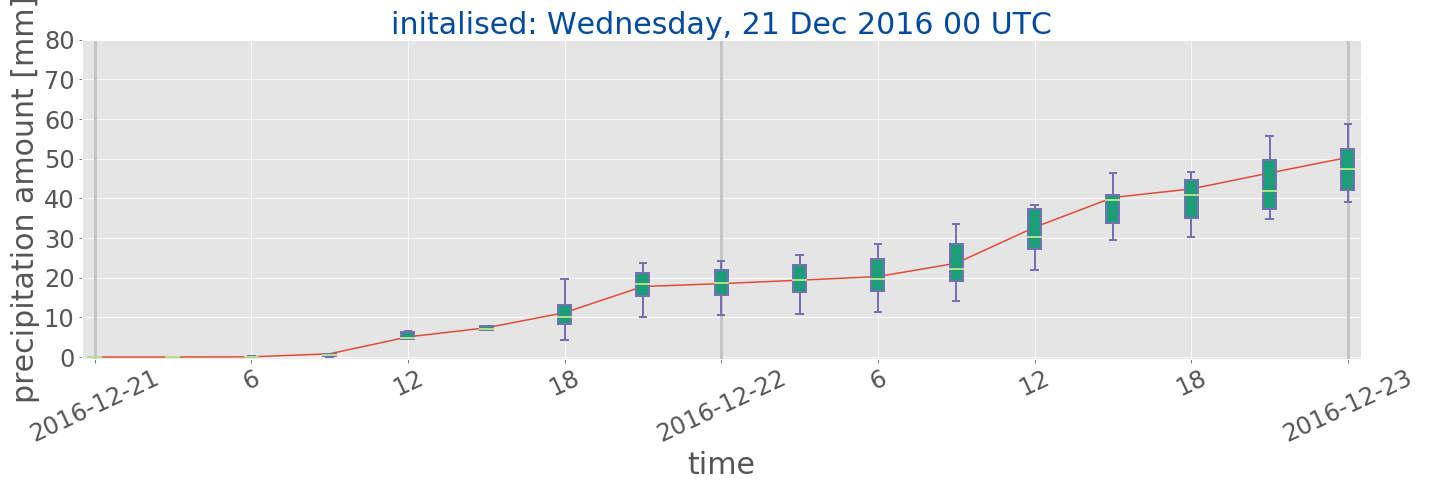
\includegraphics[width=\textwidth]{./fig_boxplot_sfc/20161221_0}
	\caption{Box-whisker-plot of the ten ensemble members of MEPS. Red line indicating the ensemble mean, lower and upper whisker the 25th and 75th percentile, respectively. Light green shows the median of all members and the box represents the middle \SI{50}{\percent} of scores of the precipitation.}\label{fig:boxplt21}
\end{figure}
%%%%%%%%%%%%%%%%%%%%%%%%%%%%%%%%%%%%%%%%%%%%%%%%%%%%%%%%%%%%%%%%%%%%%%%%%%
A box-whisker-plot shows the time evolution of the distribution of the precipitation amount made of ten ensemble members up to \SI{48}{\hour}. Since some ensemble member do not have forecast values every hour provides the box-whisker-plot in \Cref{fig:boxplt21} information every \SI{3}{\hour}. The red line shows the ensemble mean of all ten members. The short light green horizontal line is showing the median, wide vertical box represents the 25th and 75th percentiles, and minimum and maximum values are indicated by the vertical lines.
\\
The box-whisker-plot in \Cref{fig:boxplt21} shows the distribution of the ten ensemble members. In the first \SI{15}{\hour} of the forecast time agree all members well, since the box and whiskers are narrow. With increasing forecast time, increases the uncertainty. After \SI{33}{\hour} is the ensemble mean slightly higher than the median of the data. This shift is associated with the one ensemble member being an outlier.
In general can the surface forecast be trusted, especially up to \SI{24}{\hour} since the values of the ensemble members are well distributed around the mean. Maximum and minimum are not having a too large difference which also shows the small spread between the members.
%%%%%%%%%%%%%%%%%%%%%%%%%%%%%%%%%%%%%%%%%%%%%%%%%%%%%%%%%%%%%%%%%%%%%%%%%%

%%%%%%%%%%%%%%%%%%%%%%%%%%%%%%%%%%%%%%%%%%%%%%%%%%%%%%%%%%%%%%%%%%%%%%%%%%
%%%%%%%%% surface obs %%%%%%%%%%%%%%
\subsection{Saturday, \SI{24}{\dec}}\label{sec:2412:surface}
As discussed early seems the surface precipitation amount on \SI{24}{\dec} not to be influenced by too little precipitation which \cite{muller_arome-metcoop:_2017} showed to be the case for precipitation amount up to \SI{10}{\mm}. 
%%% image surface MEPS boxplot %%%%%%%%%%%%%%%%%%%%%%%%%%%%%%%%%%%%%
\begin{figure}[t]
	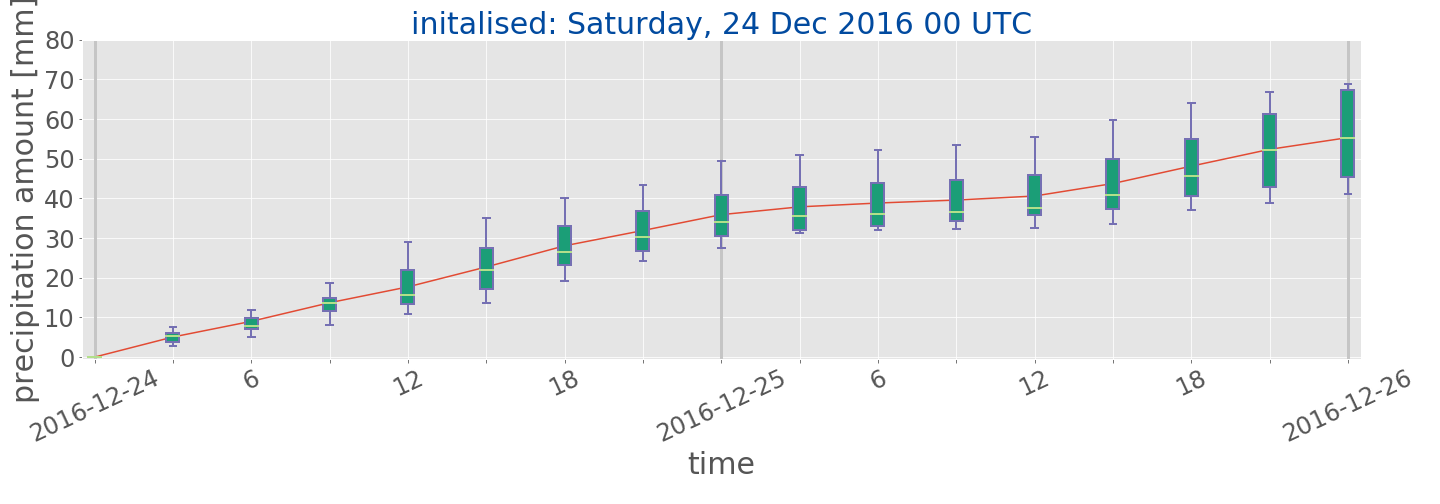
\includegraphics[width=\textwidth]{./fig_boxplot_sfc/20161224_0}
	\caption{Box-whisker-plot of the ten ensemble members of MEPS. Red line indicating the ensemble mean, lower and upper whisker the 25th and 75th percentile, respectively. Light green shows the median of all members and the box represents the middle \SI{50}{\percent} of scores of the precipitation.}\label{fig:boxplt24}
\end{figure}
%%%%%%%%%%%%%%%%%%%%%%%%%%%%%%%%%%%%%%%%%%%%%%%%%%%%%%%%%%%%%%%%%%%%%%%%%%
To understand what might have led to the overestimation of surface precipitation on the \SI{24}{\dec} in \Cref{fig:sfc_acc24}, a box-whisker-plot is presented. Compared to \SI{21}{\dec} shows the box-whisker-plot in \Cref{fig:boxplt24} an uncertainty between the ten ensemble members already after \SI{3}{\hour} forecast time. The spread between the ensemble members (shown by the minimum and maximum whiskers) seems to be wide. Not all ten members agree on the same precipitation amount as they did for example on \SI{21}{\dec}.
\\
The ensemble mean (red line) is always higher than the median and already after \SI{12}{\hour} forecast time is the median closer to the lower 25th percentile. Also, all upper whiskers are taller than the lower ones, which would follow that the ensemble members vary amongst the most positive quartile and that it is very similar for the least positive quartile group.
A comparison with \Cref{fig:sfc_acc24} shows that most of the member lie beneath the ensemble mean (dashed, blue line). On \SI{24}{\dec} the ensemble mean is much lower than the deterministic forecast, which lies closer to the 50th percentile. This is not for all days the case, on most of the days is the ensemble mean either similar or a little less to the deterministic forecast. Since the deterministic forecast, black line in \Cref{fig:sfc_acc24}, is in the upper percentile compared to its perturbed members it follows that for this forecast the deterministic forecast was not the best guess for the surface accumulation and by using the 'wrong' initial state it can have led to larger miscalculations. Therefore, it would be interesting to perform a new deterministic forecast and its associated perturbations to see if a change in choosing another initial state results in a similar measured precipitation amount at the ground.
\\
\\
The uncertainty appearing already after \SI{3}{\hour} can be associated with a too long spin-up time of MEPS. MEPS usually has a spin-up time of about three hours on \SI{25}{\dec} this might have been longer and followed by poorer initial conditions. To represent the surface accumulation well, the model systems needs to be spin-up. The regional model MEPS needs initial and boundary conditions from ECMWF before it can produce forecasts. Since initial conditions such as observations have uncertainties as well as the model has mistrust and needs to approach its own climatology, a model has to stabilize before the simulations can be trusted. The spin-up time varies depending on the quality of the initial and boundary conditions. Apparently, it seems, that the initial and boundary conditions for MEPS were not perfect on \SI{24}{\dec} at \SI{0}{\UTC} since the deterministic and perturbed members seem not to have stabilised yet and show uncertainties in \Cref{fig:boxplt24} from early on.  At this point it might be interesting to re-run the initialisation again with all available observations to see, if that might have an influence on the overestimation observed in \Cref{fig:sfc_acc24}. It might not necessarily be the observations. Since, ECMWF is the boundary condition of MEPS it could also be that the ECMWF forecast did not have reached its stabilised state when MEPS was initiated.
\\
The uncertainty might also have resulted from the fact, that the precipitation around \SI{0}{\UTC} on \SI{24}{\dec} was higher than on the previous days (see, \Cref{fig:TPU}). Where on the previous days the hourly precipitation around \SI{0}{\UTC} was less intense might a big accretion have followed an uncertainty already after \SI{3}{\hour}. MEPS initialised on \SI{24}{\dec} at \SI{0}{\UTC} might have accounted for an additional precipitation at \SI{12}{\UTC} on \SI{24}{\dec} and that led to the strong increase at \SI{13}{\UTC}. This might be a local effect, that a precipitation cell in the model was spatially misplaced or a by a few kilometres or a higher precipitation amount was expected by the model and actually did not occur at Haukeliseter rather at another site close to Haukeliseter, and followed that strong increase after noon. 
\\
It is therefore important as the double fence construction or measurements from the MRR to give models a good initial condition from observations, so that spin-up time can be reduced and model initialisation start at a realistic state.

%%%%%%%%%%%%%%%%%%%%%%%%%%%%%%%%%%%%%%%%%%%%%%%%%%%%%%%%%%%%%%%%%%%%%%%%%%
%%%%%%%%% surface obs %%%%%%%%%%%%%%
\subsection{Sunday, \SI{25}{\dec}}\label{sec:2512:surface}
On \SI{25}{\dec} the surface accumulation for the first \SI{12}{\hour} is \SI{4.3}{\mm} (see \Cref{tab:sfc_acc}). \cite{muller_arome-metcoop:_2017} stated that the deterministic forecast is showing some overestimation if the \SI{12}{\hour} accumulation is less than \SI{10}{\mm}. Even though the surface accretion is smaller than \SI{10}{\mm} might that not correlate with miscalculation on \SI{25}{\dec}. The overestimation started to be pronounced \SI{13}{\hour} after the initialisation in \Cref{fig:sfc_acc25}.
%
%%% image surface MEPS boxplot %%%%%%%%%%%%%%%%%%%%%%%%%%%%%%%%%%%%%
\begin{figure}[t]
	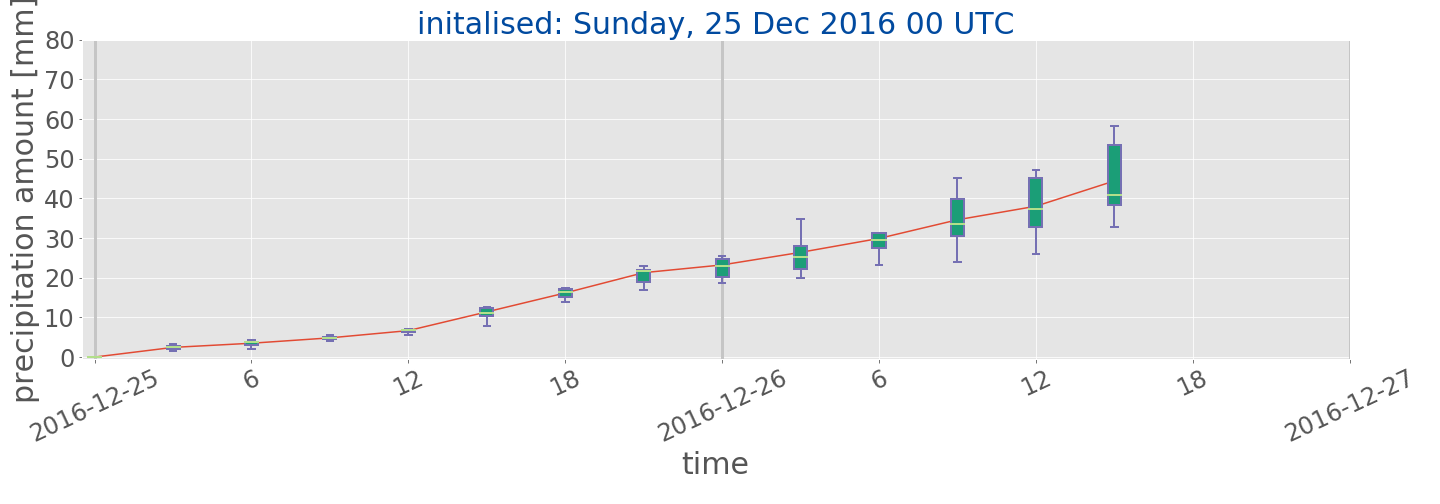
\includegraphics[width=\textwidth]{./fig_boxplot_sfc/20161225_0}
	\caption{Box-whisker-plot of the ten ensemble members of MEPS initialised on \SI{25}{\dec} at \SI{0}{\UTC}. Red line indicating the ensemble mean, lower and upper whisker the 25th and 75th percentile, respectively. Light green shows the median of all members and the box represents the middle \SI{50}{\percent} of scores of the precipitation.}\label{fig:boxplt25}
\end{figure}
%%%%%%%%%%%%%%%%%%%%%%%%%%%%%%%%%%%%%%%%%%%%%%%%%%%%%%%%%%%%%%%%%%%%%%%%%%
%
Compared to \SI{24}{\dec} are the box-whiskers narrower for the first \SI{30}{\hour} on \SI{25}{\dec} in \Cref{fig:boxplt25}. The overestimation started to occur around \SI{13}{\UTC} in \Cref{fig:sfc_acc25}. As \Cref{fig:boxplt25} shows, increases the uncertainty in the forecast after \SI{15}{\UTC}. In general agree median and mean well for the entire period of a \SI{48}{\hour} forecast. After \SI{39}{\hour} prediction time is the mean much higher than the median and closer to the lower 25th percentile in \Cref{fig:boxplt25}. It seems, that all ten ensemble members agree well on the prediction and nevertheless overestimates MEPS the surface accumulation. It shows that the MEPS estimation follows the double fence amount, just not as high. 
\\
In this case it might have been a miscalculation of the occurrence and amount of the precipitation. From the box-whisker-plot (\Cref{fig:boxplt25}) it seems not to be an initialisation problem, since all members agree and the fact that the ensemble mean agrees with the deterministic run. On \SI{25}{\dec} it was expected from the weather maps that a warm front, the warm sector, and a cold front are going to pass. MEPS might have misinterpreted this passages and expected more, probably liquid precipitation associated with the warm front. 
An error associated with the spin-up time of MEPS is not totally excluded. Since the box-whisker-plot shows a good agreement between all members it is not very likely that this was the problem on \SI{25}{\dec}
\\
That the retrieval underestimates the surface precipitation in the afternoon on \SI{25}{\dec} is due to the total negligence  of liquid precipitation if the surface temperature exceeds \SI{2}{\celsius}. Since the optimal estimation retrieval only uses the moist adiabatic lapse rate of \SI{5}{\kelvin\per\km} it might not represent the true state of the atmosphere. Therefore, a use of radiosonde can provide a real structure of the vertical temperature profile which then can help to give real estimations of solid precipitation in the vertical.
After the optimal estimation retrieval is fully developed it will be interesting to study the combination of liquid and snowfall precipitation. 

%%%%%%%%%%%%%%%%%%%%%%%%%%%%%%%%%%%%%%%%%%%%%%%%%%%%%%%%%%%%%%%%%%%%%%%%%%

%%%%%%%%%%%%%%%%%%%%%%%%%%%%%%%%%%%%%%%%%%%%%%%%%%%%%%%%%%%%%%%%%%%%%%%%%%
%%%%%%%%% SWC COMPARISON %%%%%%%%%%%%%%
% !TeX spellcheck = en_GB
\section{SWC and SWP from MEPS and the optimal estimation retrieval}
Images for the liquid water content evaluated in MEPS can be found in \Cref{app:LWP_MEPS}. 

%%% table SWP and LWP max %%%%%%%%%%%%%%%%%%%%%%%%%%%%%%%%%%%%%
% !TeX spellcheck = en_GB
\begin{table}[h!]
	\begin{center}
		\caption{Maximum values of the snow water and liquid water content from the retrieval and MEPS}\label{tab:max_val}
		\begin{tabular}{ll|c|c|c|c|c|c} 
			\hline \hline
			& & \textbf{SWC}  & \textbf{HEIGHT}  & \textbf{TIME} & \textbf{LWC}  & \textbf{HEIGHT}  & \textbf{TIME}  \\
			& & [\SI{}{\kg\per\cubic\meter}] & [\SI{}{\meter}] &  & [\SI{}{\kg\per\cubic\meter}] & [\SI{}{\meter}] &   \\
			\hline \hline
			\multicolumn{8}{c}{\textbf{Wed, 21 Dec 2016}} \\ \hline
			\multicolumn{2}{l|}{RETRIEVAL} & 1.08 & 600.0 & \SI{16}{\UTC} & & & \\
			\multicolumn{2}{l|}{MEPS} &  &  & & & & \\
			& ensemble mean & \num{1.24} & \num{1400.0} & \SI{20}{\UTC} & & & \\
			& control & \num{2.11} & \num{1400.0} & \SI{20}{\UTC} & \num{0.15} & \num{2200.0} & \SI{23}{\UTC}\\ \hline \hline
			\multicolumn{8}{c}{\textbf{Thu, 22 Dec 2016}} \\ \hline
			\multicolumn{2}{l|}{RETRIEVAL} & \num{1.46} & \num{1200.0} & \SI{10}{\UTC} & & & \\
			\multicolumn{2}{l|}{MEPS} &  &  & & & & \\
			& ensemble mean & \num{1.54} & \num{2200.0} & \SI{14}{\UTC} & & & \\
			& control & \num{1.35} & \num{1400.0} & \SI{12}{\UTC} & \num{0.20} & \num{2000.0} & 0\SI{02}{\UTC} \\ \hline \hline
			\multicolumn{8}{c}{\textbf{Fri, 23 Dec 2016}} \\ \hline
			\multicolumn{2}{l|}{RETRIEVAL} & \num{0.91} & \num{600.0} & \SI{23}{\UTC} & & & \\
			\multicolumn{2}{l|}{MEPS} &  &  & & & & \\
			& ensembel mean & \num{0.54} & \num{400.0} & \SI{20}{\UTC} & & & \\
			& control & \num{0.54} & \num{400.0} & \SI{20}{\UTC} & \num{0.14} & \num{1000.0} & \SI{15}{\UTC} \\ \hline \hline
			\multicolumn{8}{c}{\textbf{Sat, 24 Dec 2016}} \\ \hline
			\multicolumn{2}{l|}{RETRIEVAL} & \num{1.39} & \num{1000.0} & 0\SI{06}{\UTC} & & & \\
			\multicolumn{2}{l|}{MEPS} &  &  & & & & \\
			& ensembel mean & \num{0.70} & \num{1400.0} & 0\SI{07}{\UTC} & & & \\
			& control & \num{0.73} & \num{1400.0} & \SI{17}{\UTC} & \num{0.33} & \num{1200.0} & 0\SI{09}{\UTC} \\ \hline \hline
			\multicolumn{8}{c}{\textbf{Sun, 25 Dec 2016}} \\ \hline
			\multicolumn{2}{l|}{RETRIEVAL} & \num{0.69} & \num{1400.0} & \SI{21}{\UTC} & & & \\
			& ensembel mean & \num{0.44} & \num{400.0} & \SI{20}{\UTC} & & & \\
			& control & \num{0.50} & \num{800.0} & \SI{20}{\UTC} & \num{0.34} & \num{200.0} & \SI{17}{\UTC} \\ \hline \hline
			\multicolumn{8}{c}{\textbf{Mon, 26 Dec 2016}} \\ \hline
			\multicolumn{2}{l|}{RETRIEVAL} & \num{1.25} & \num{600.0} & \SI{15}{\UTC} & & & \\
			& ensembel mean & \num{0.95} & \num{800.0} & \SI{16}{\UTC} & & & \\
			& control & \num{1.55} & \num{1000.0} & \SI{11}{\UTC} & \num{0.17} & \num{2400.0} & 0\SI{09}{\UTC} \\ \hline \hline
			\multicolumn{8}{c}{\textbf{Tue, 27 Dec 2016}} \\ \hline
			\multicolumn{2}{l|}{RETRIEVAL} & -- & -- & -- & & & \\
			& ensembel mean & \num{0.16} & \num{400.0} & 0\SI{00}{\UTC} & & & \\
			& control & \num{0.16} & \num{400.0} & 0\SI{00}{\UTC} & \num{0.25} & \num{800.0} & \SI{23}{\UTC} \\ \hline \hline
		\end{tabular}
	\end{center}
\end{table}
%%%%%%%%%%%%%%%%%%%%%%%%%%%%%%%%%%%%%%%%%%%%%%%%%%%%%%%%%%%%%%%%%%%%%%%%%%

%%% image SWC, SWP Retrieval MEPS comparison %%%%%%%%%%%%%%%%%%%%%%%%%%%%%%%%%%%%%
% !TeX spellcheck = en_GB
%\begin{landscape}
\begin{figure}[h]
	\centering
    	% 21/12
		\begin{subfigure}[b]{0.8\textwidth}
			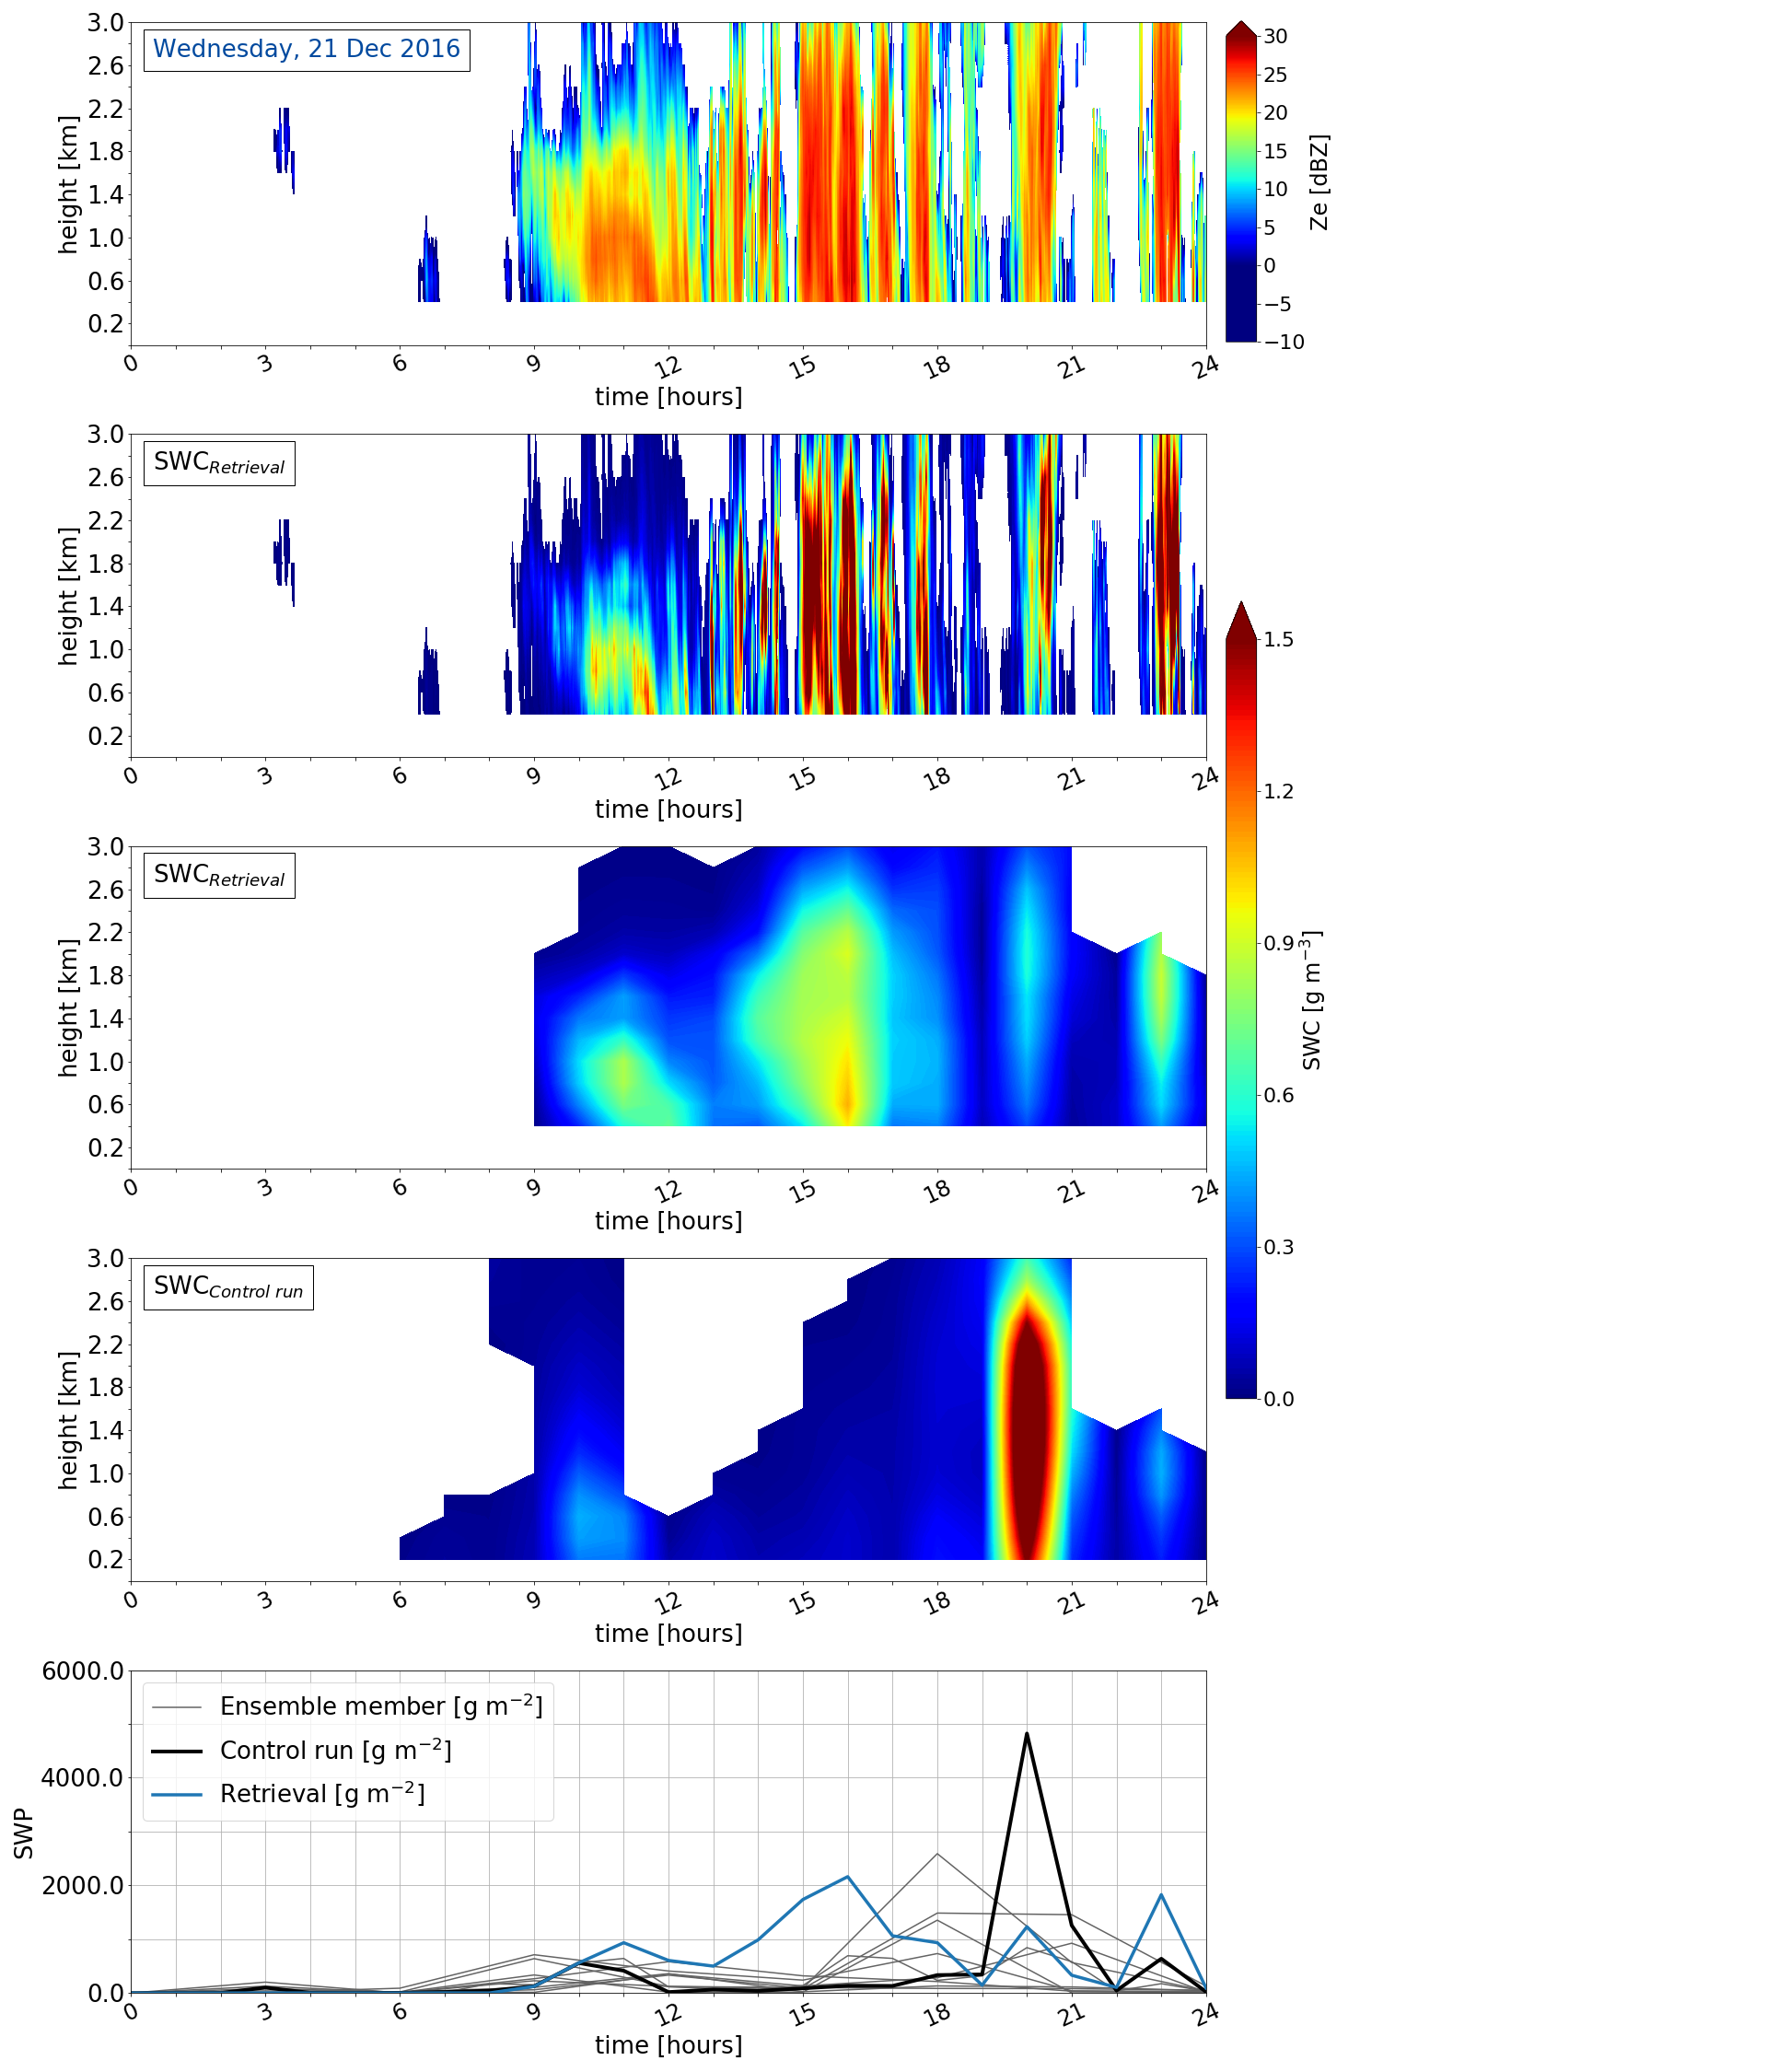
\includegraphics[trim={0.5cm 0.5cm 17.5cm .5cm},clip,width=\textwidth]{./fig_SWC/20161221}
			\caption{Wednesday, \SI{21}{\dec}}\label{fig:SWC21}
		\end{subfigure}
\end{figure}
\begin{figure}\ContinuedFloat
   	\centering
		% 22/12
	\begin{subfigure}[b]{0.8\textwidth}
			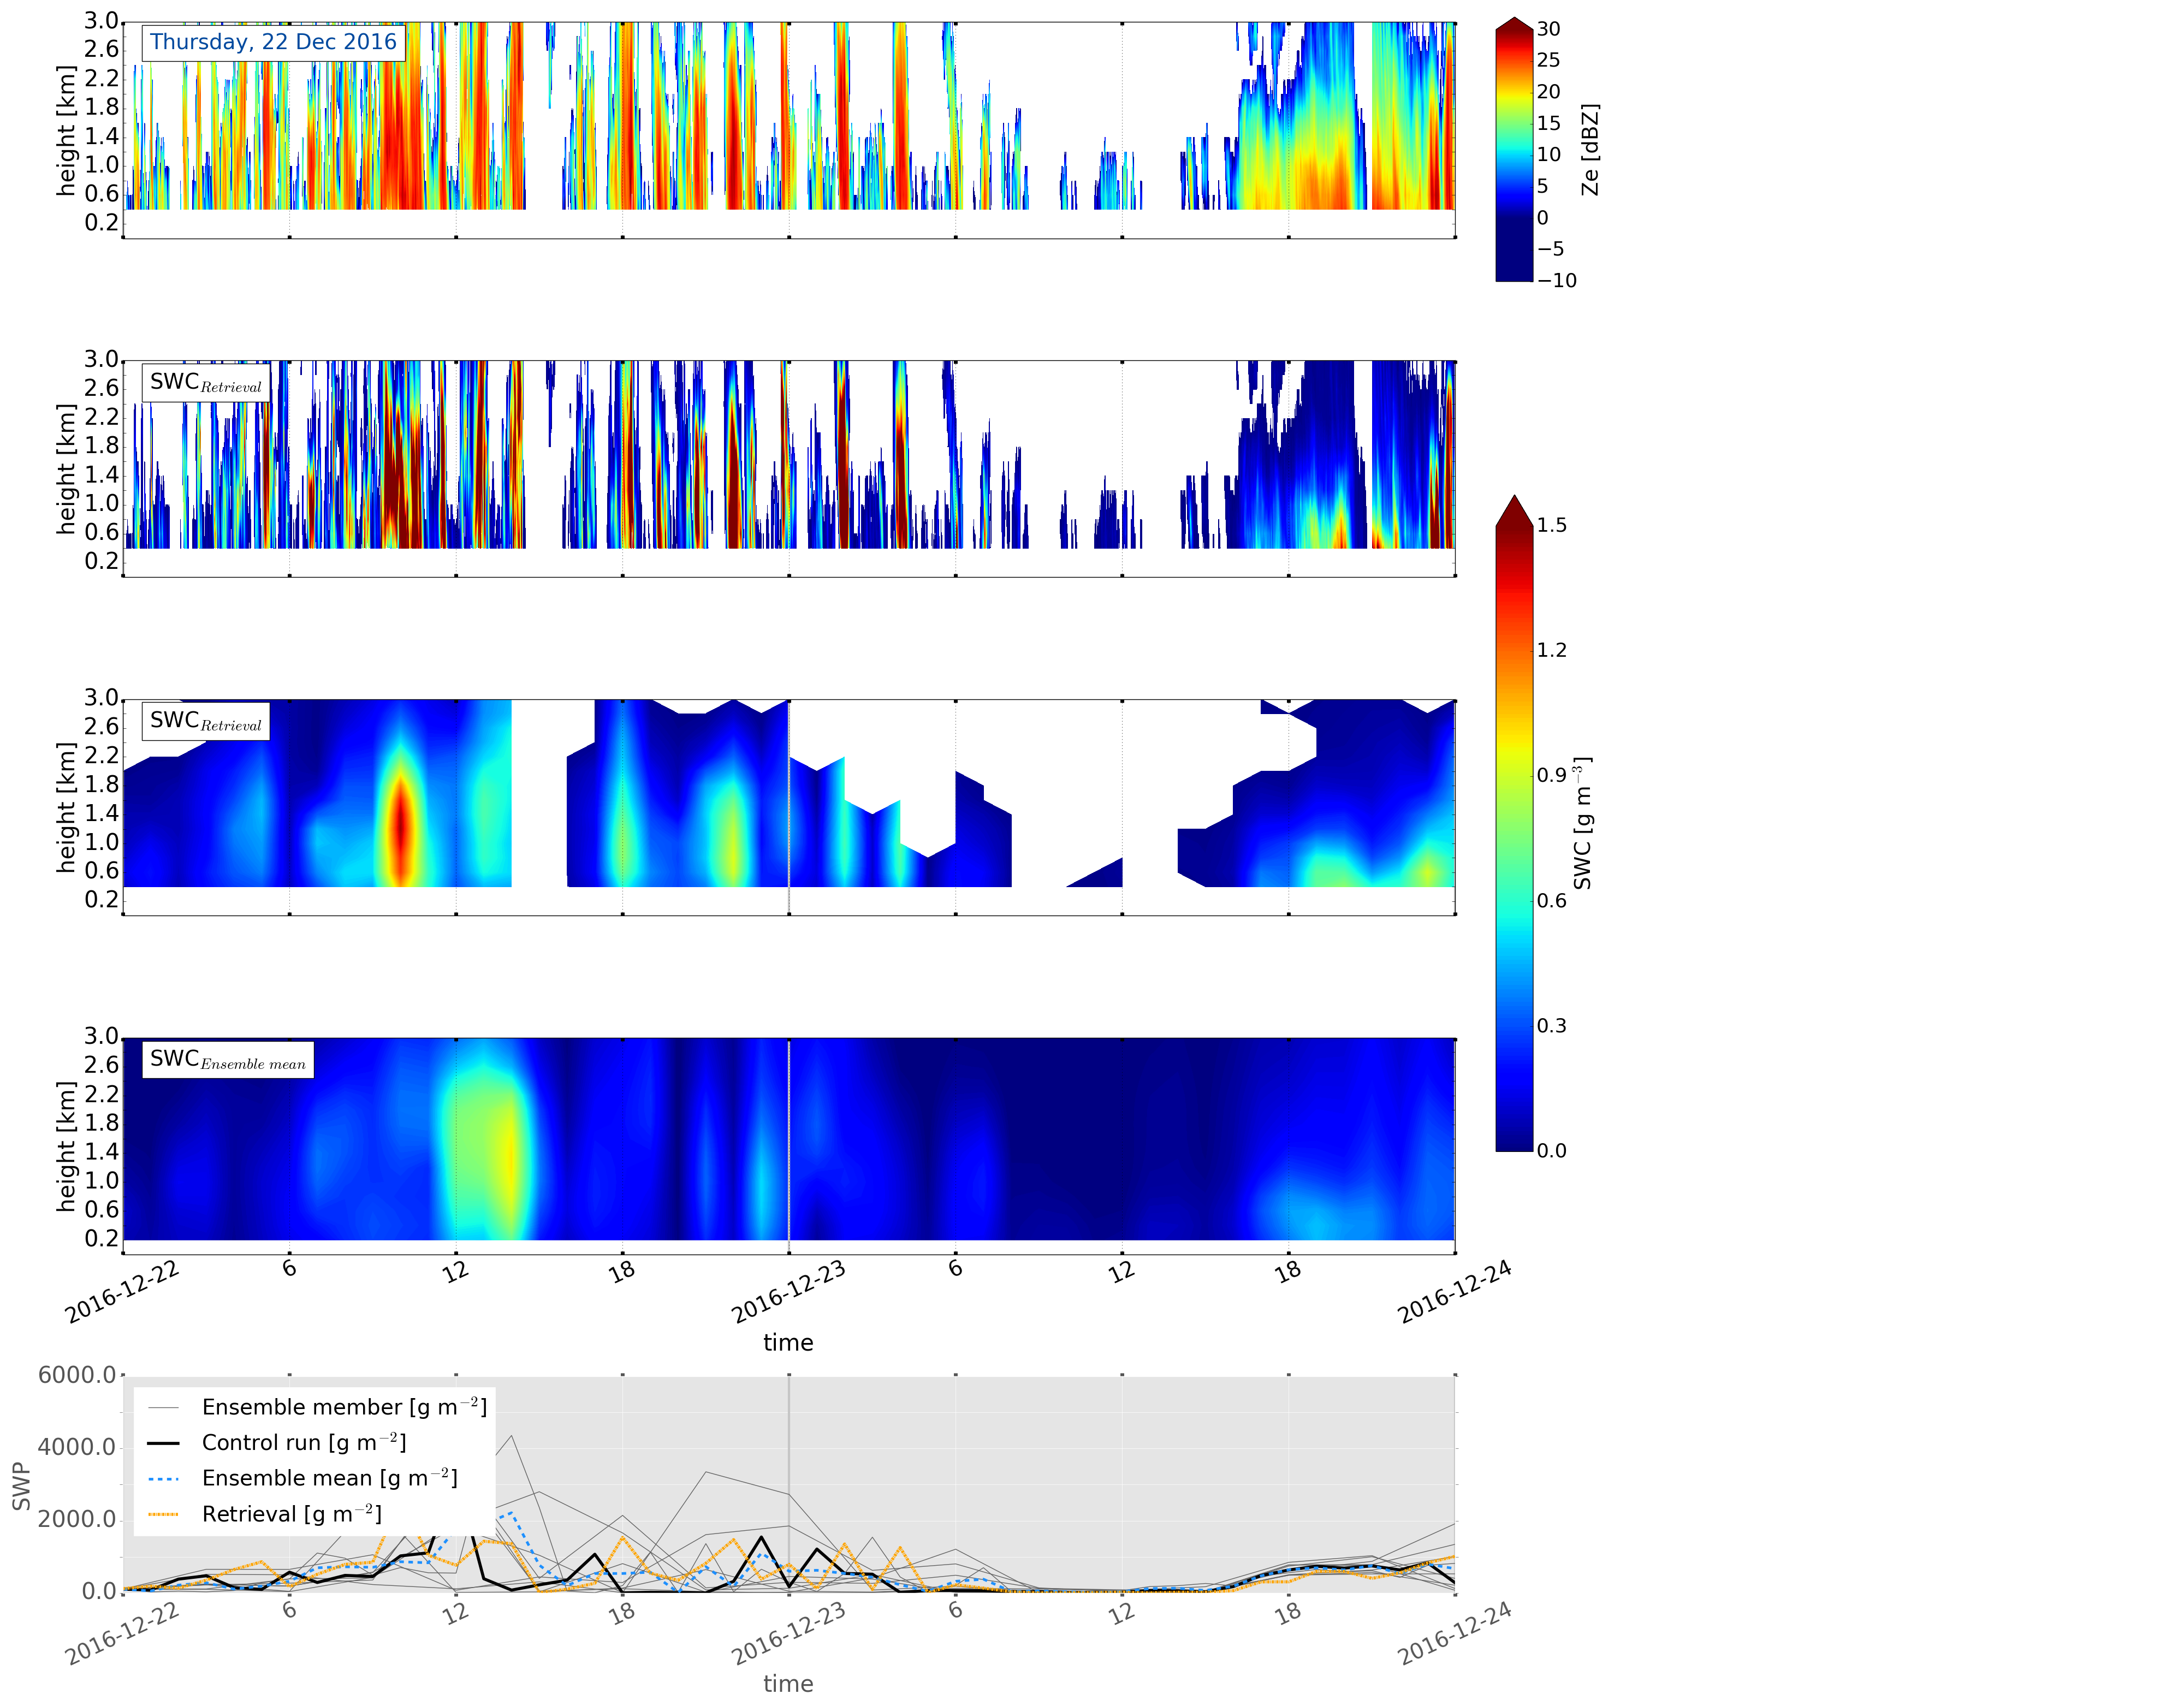
\includegraphics[trim={0.5cm 0.5cm 17.5cm .5cm},clip,width=\textwidth]{./fig_SWC/20161222}
			\caption{Thursday, \SI{22}{\dec}}\label{fig:SWC22}
		\end{subfigure}
	\end{figure}
    \begin{figure}\ContinuedFloat
   		\centering
		% 23/12
		\begin{subfigure}[b]{0.8\textwidth}
			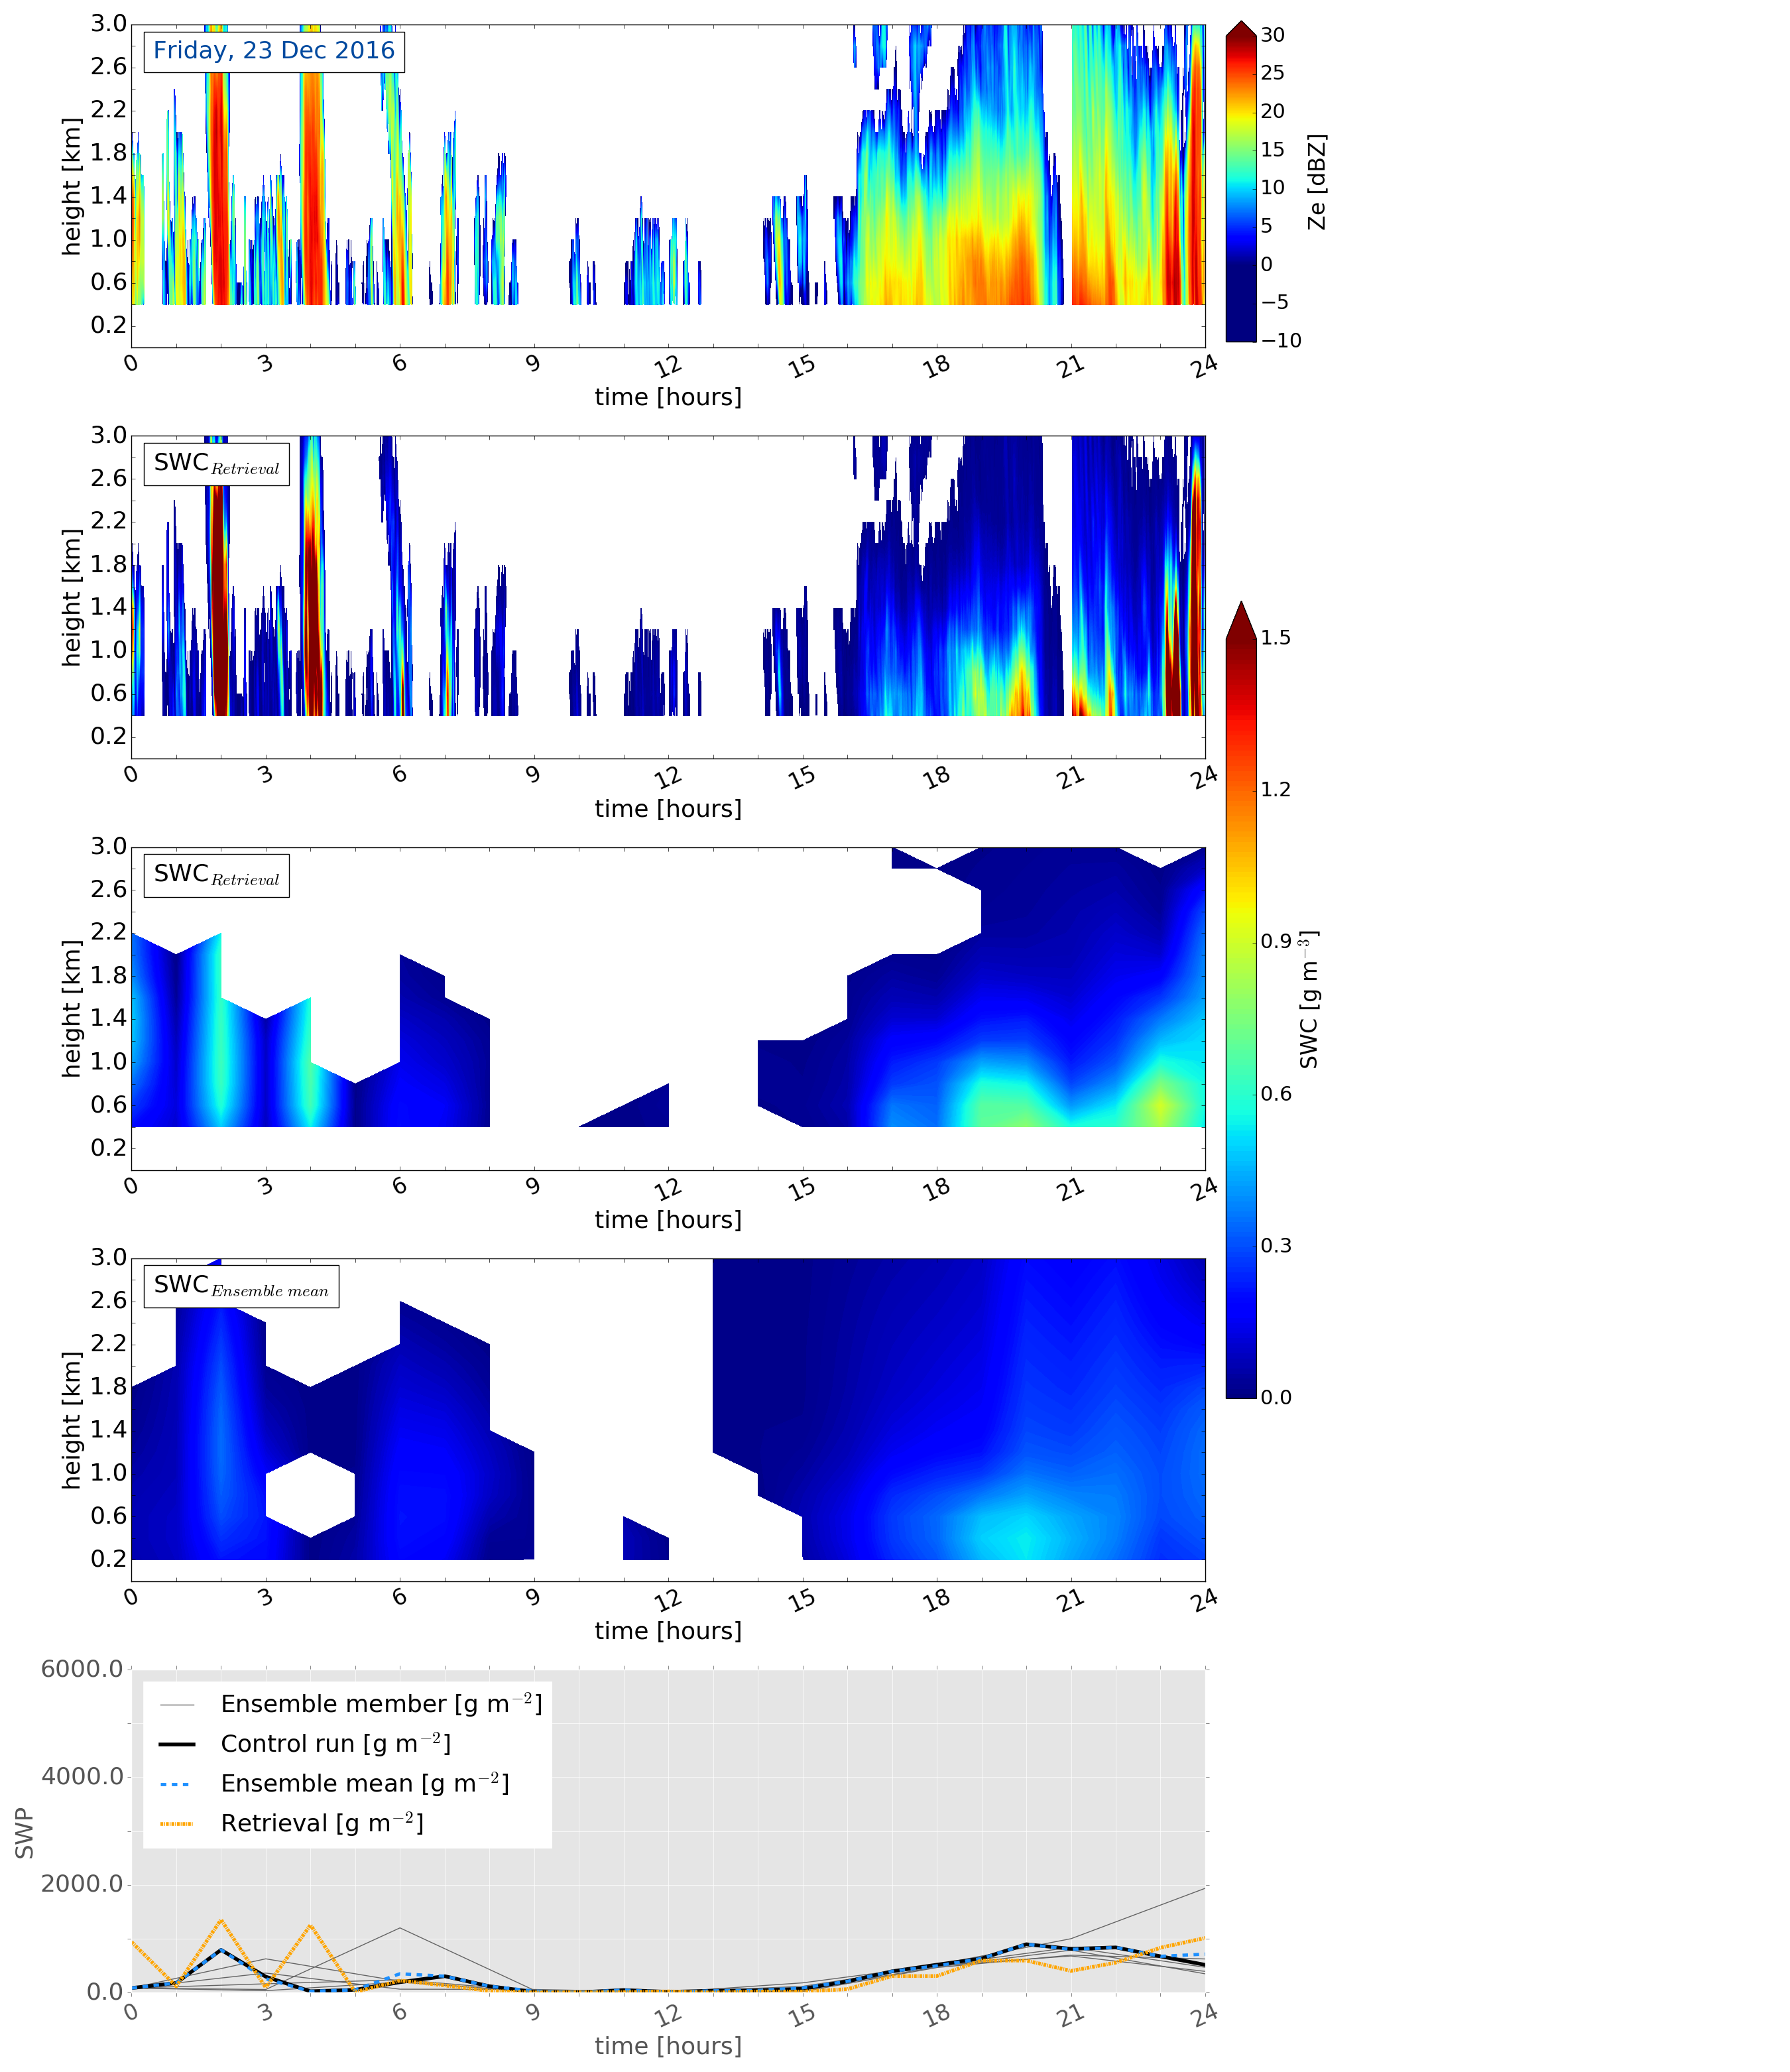
\includegraphics[trim={0.5cm 0.5cm 17.5cm .5cm},clip,width=\textwidth]{./fig_SWC/20161223}
			\caption{Friday, \SI{23}{\dec}}\label{fig:SWC23}
		\end{subfigure}
	\end{figure}
    \begin{figure}\ContinuedFloat
   		\centering
		% 24/12
		\begin{subfigure}[b]{0.8\textwidth}
			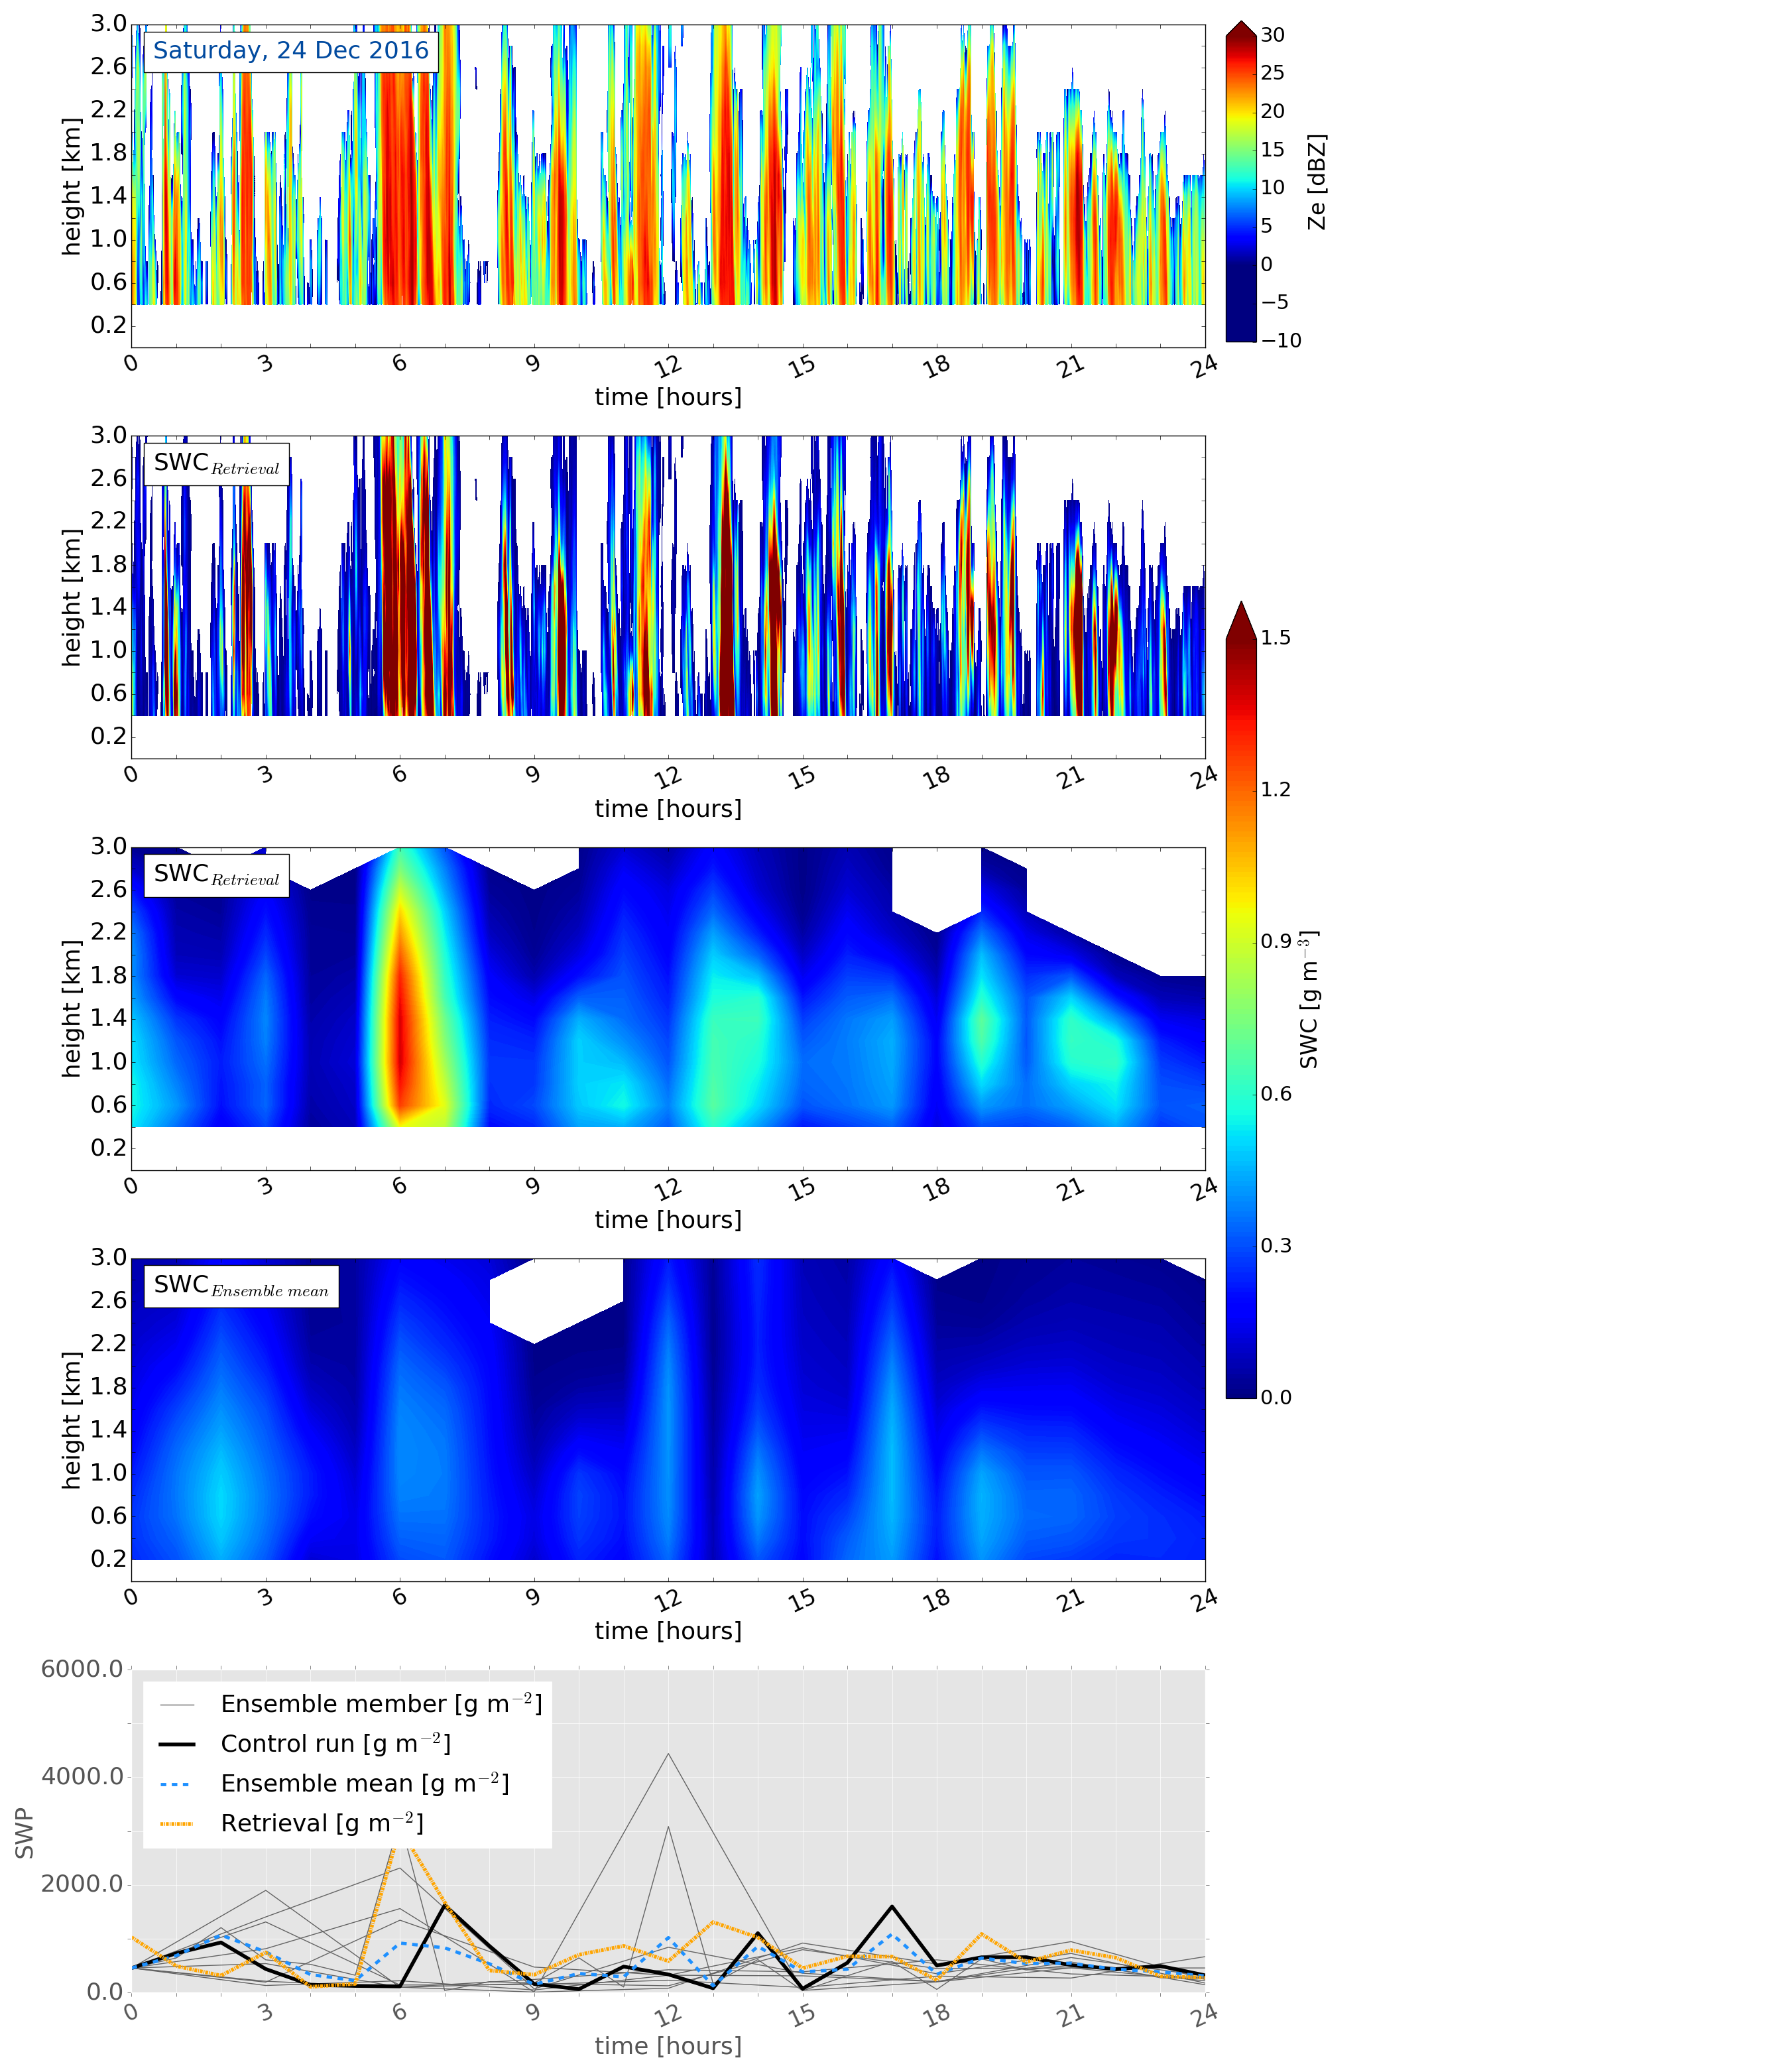
\includegraphics[trim={0.5cm 0.5cm 17.5cm .5cm},clip,width=\textwidth]{./fig_SWC/20161224}
			\caption{Saturday, \SI{24}{\dec}}\label{fig:SWC24}
		\end{subfigure}
	\end{figure}
    \begin{figure}\ContinuedFloat
   		\centering
		% 25/12
		\begin{subfigure}[b]{0.8\textwidth}
			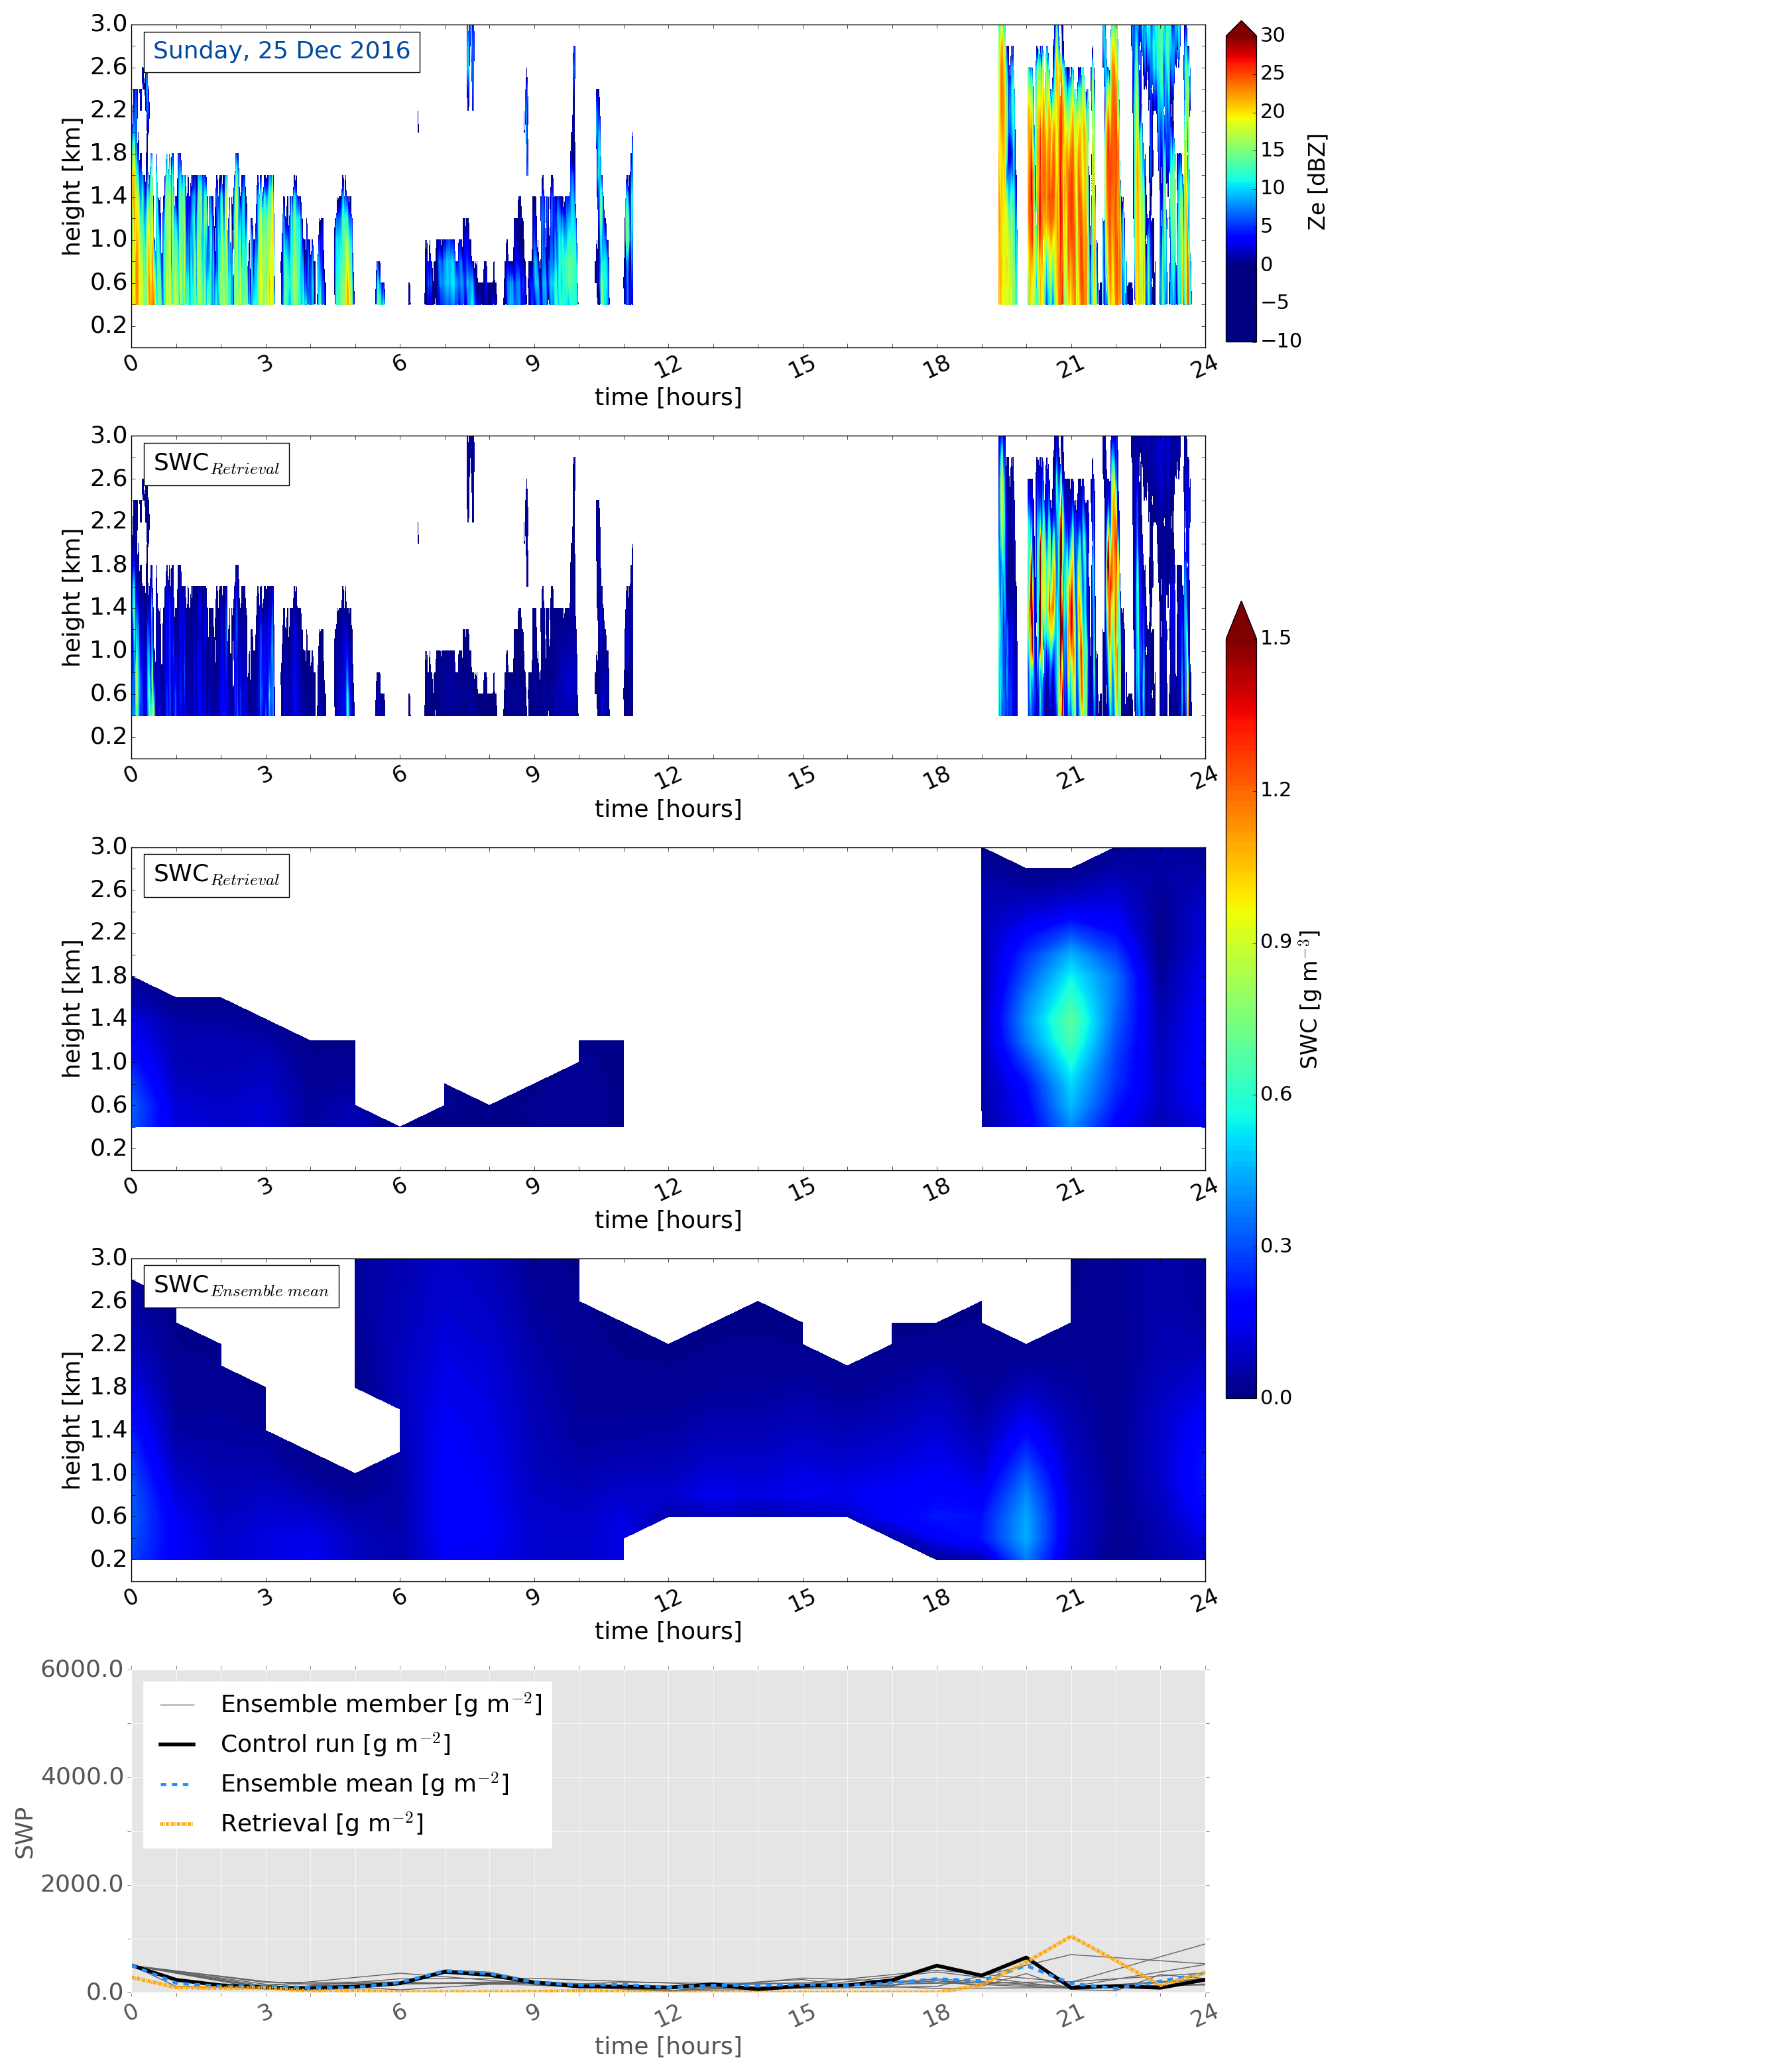
\includegraphics[trim={0.5cm 0.5cm 17.5cm .5cm},clip,width=\textwidth]{./fig_SWC/20161225}
			\caption{Sunday, \SI{25}{\dec}}\label{fig:SWC25}
		\end{subfigure}
	\end{figure}
    \begin{figure}\ContinuedFloat
   		\centering
		% 26/12
		\begin{subfigure}[b]{0.8\textwidth}
			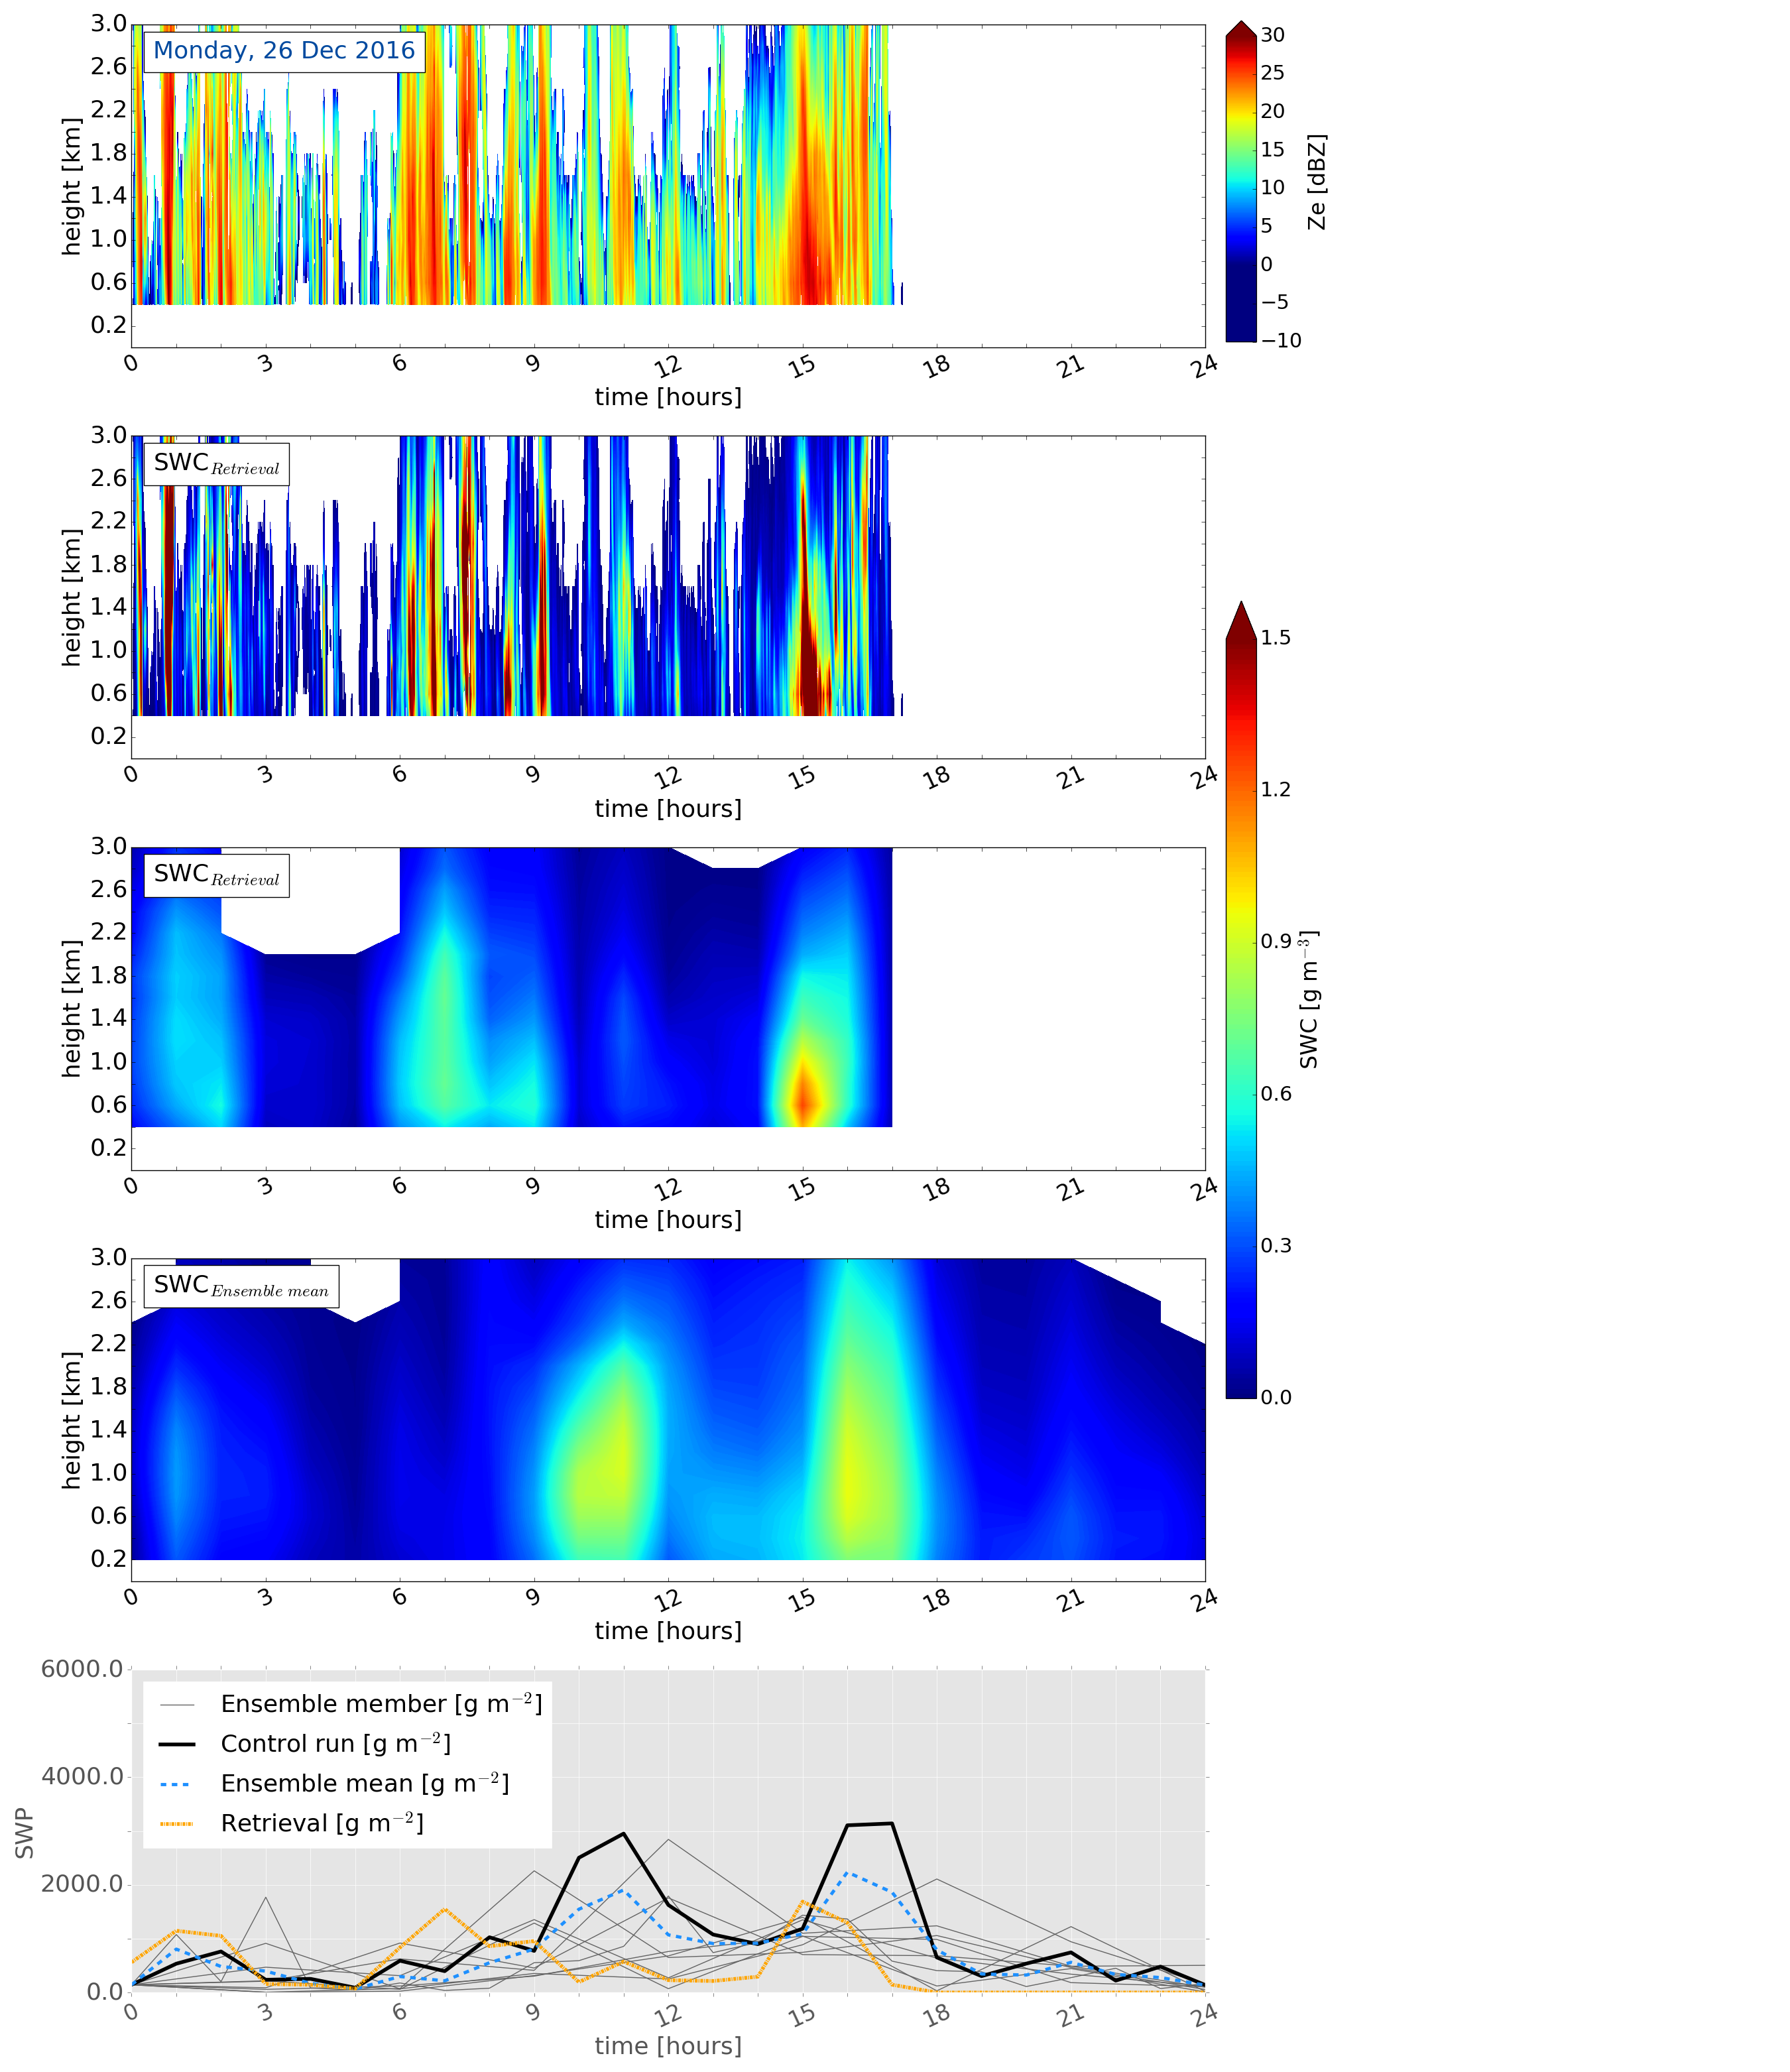
\includegraphics[trim={0.5cm 0.5cm 17.5cm .5cm},clip,width=\textwidth]{./fig_SWC/20161226}
			\caption{Monday, \SI{26}{\dec}}\label{fig:SWC26}
		\end{subfigure}
        \caption{Upper panel: MRR reflectivity in \SI{}{\dB Z}. 2nd panel: SWC optimal estimation retrieval output every second in \SI{}{\gram\per\cubic\metre}. 3rd panel: hourly-averaged SWC optimal estimation retrieval output. 4th panel: \SI{200}{\metre}-averaged SWC deterministic forecast from MEPS. Lowest panel: SWP from MEPS, initialised at \SI{00}{\UTC}. Black line represents the deterministic forecast and the grey lines the nine perturbed members. In blue the SWP from the averaged retrieval output.}\label{fig:SWC}
	\end{figure}
	

%%%%%%%%%%%%%%%%%%%%%%%%%%%%%%%%%%%%%%%%%%%%%%%%%%%%%%%%%%%%%%%%%%%%%%%%%%




%%%%%%%%%%%%%%%%%%%%%%%%%%%%%%%%%%%%%%%%%%%%%%%%%%%%%%%%%%%%%%%%%%%%%%%%%%

%\newpage
%%%%%%%%%%%%%%%%%%%%%%%%%%%%%%%%%%%%%%%%%%%%%%%%%%%%%%%%%%%%%%%%%%%%%%%%%%
%%%%%%%%% ensemble verification %%%%%%%%%%%%%%
% !TeX spellcheck = en_GB
\subsection{Verification of MEPS ensemble members}\label{sec:variation}
%%%%%%%%% image SWC retrieved %%%%%%%%%%%%%%
% !TeX spellcheck = en_GB

%%%%%%%
\begin{figure}[t]
	\centering
    % 20/12
		\begin{subfigure}[t]{\textwidth}		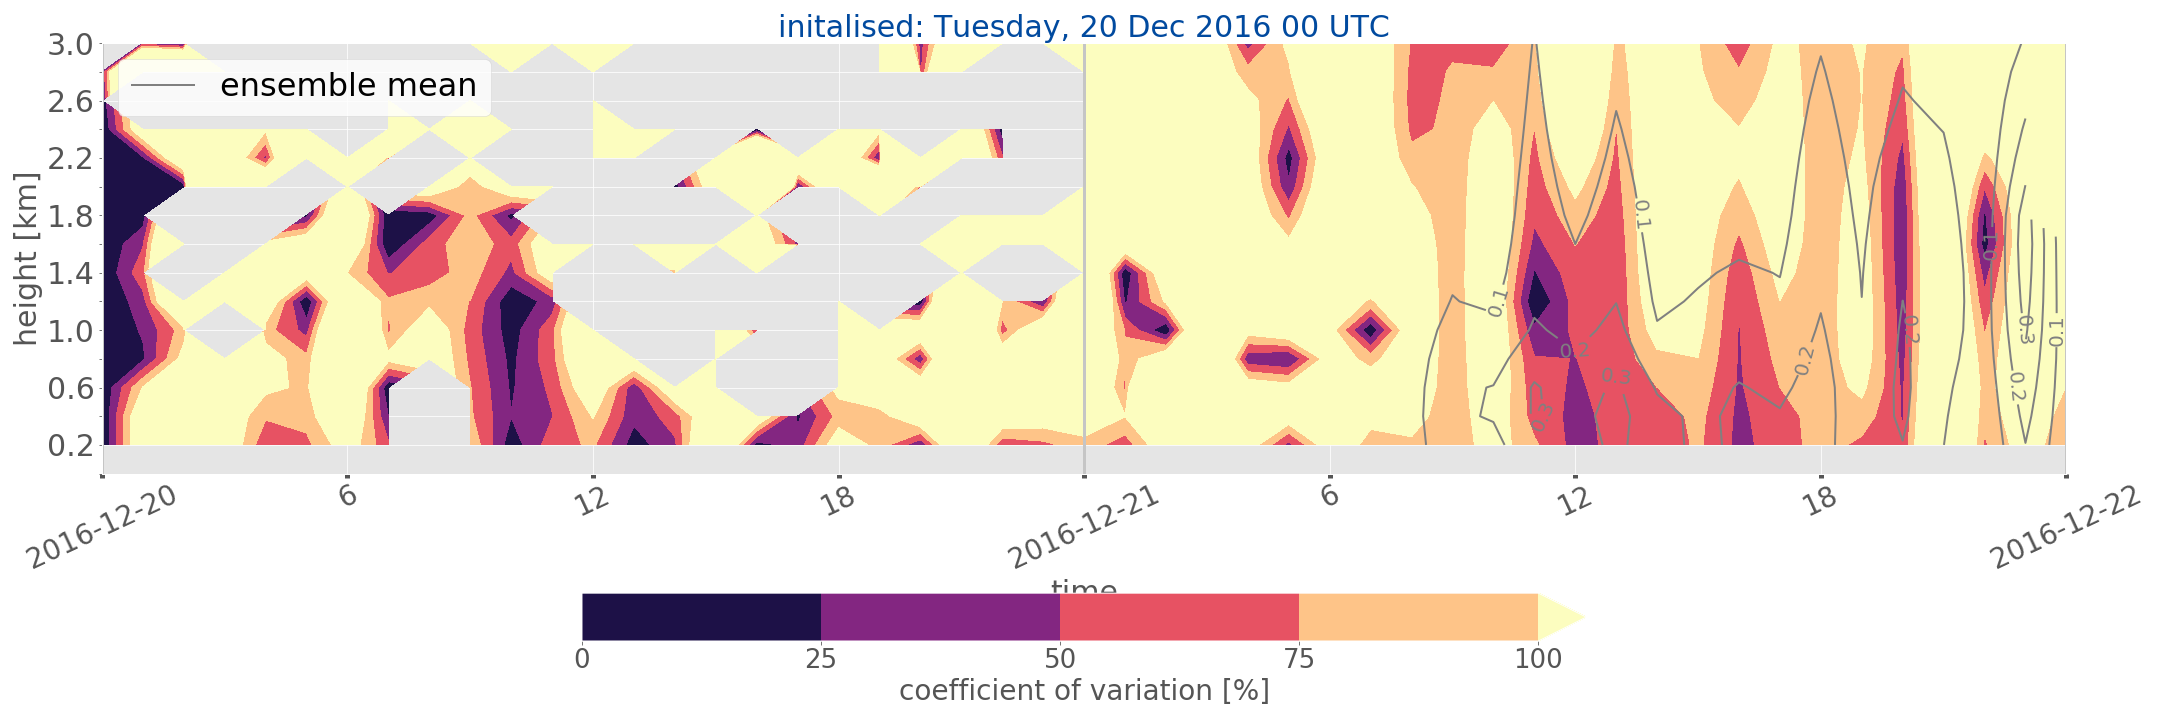
\includegraphics[trim={0.cm 5.3cm 0cm 0cm},clip,width=\textwidth]{./fig_variation/20161220}
			\caption{}\label{fig:ens_vari20}
		\end{subfigure}
%\end{figure}
%\begin{figure}\ContinuedFloat
    % 21/12
		\begin{subfigure}[t]{\textwidth}		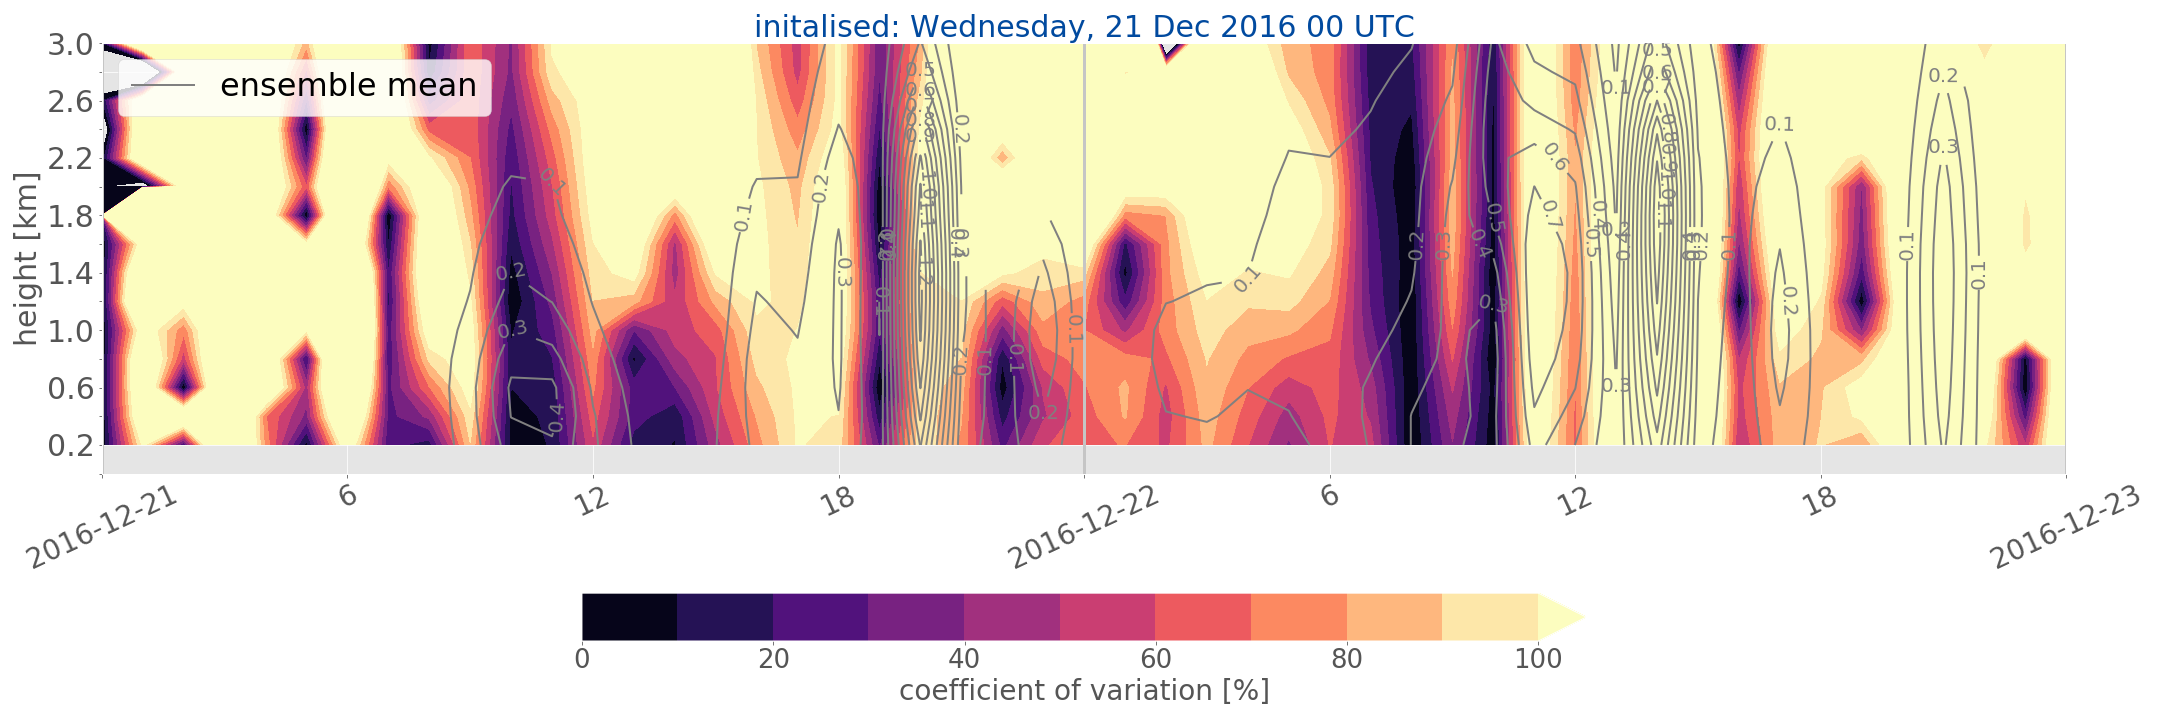
\includegraphics[trim={0.cm 5.3cm 0cm 0cm},clip,width=\textwidth]{./fig_variation/20161221}
			\caption{}\label{fig:ens_vari21}
		\end{subfigure}
       
       % colourbar
     	\begin{subfigure}[t]{\textwidth}		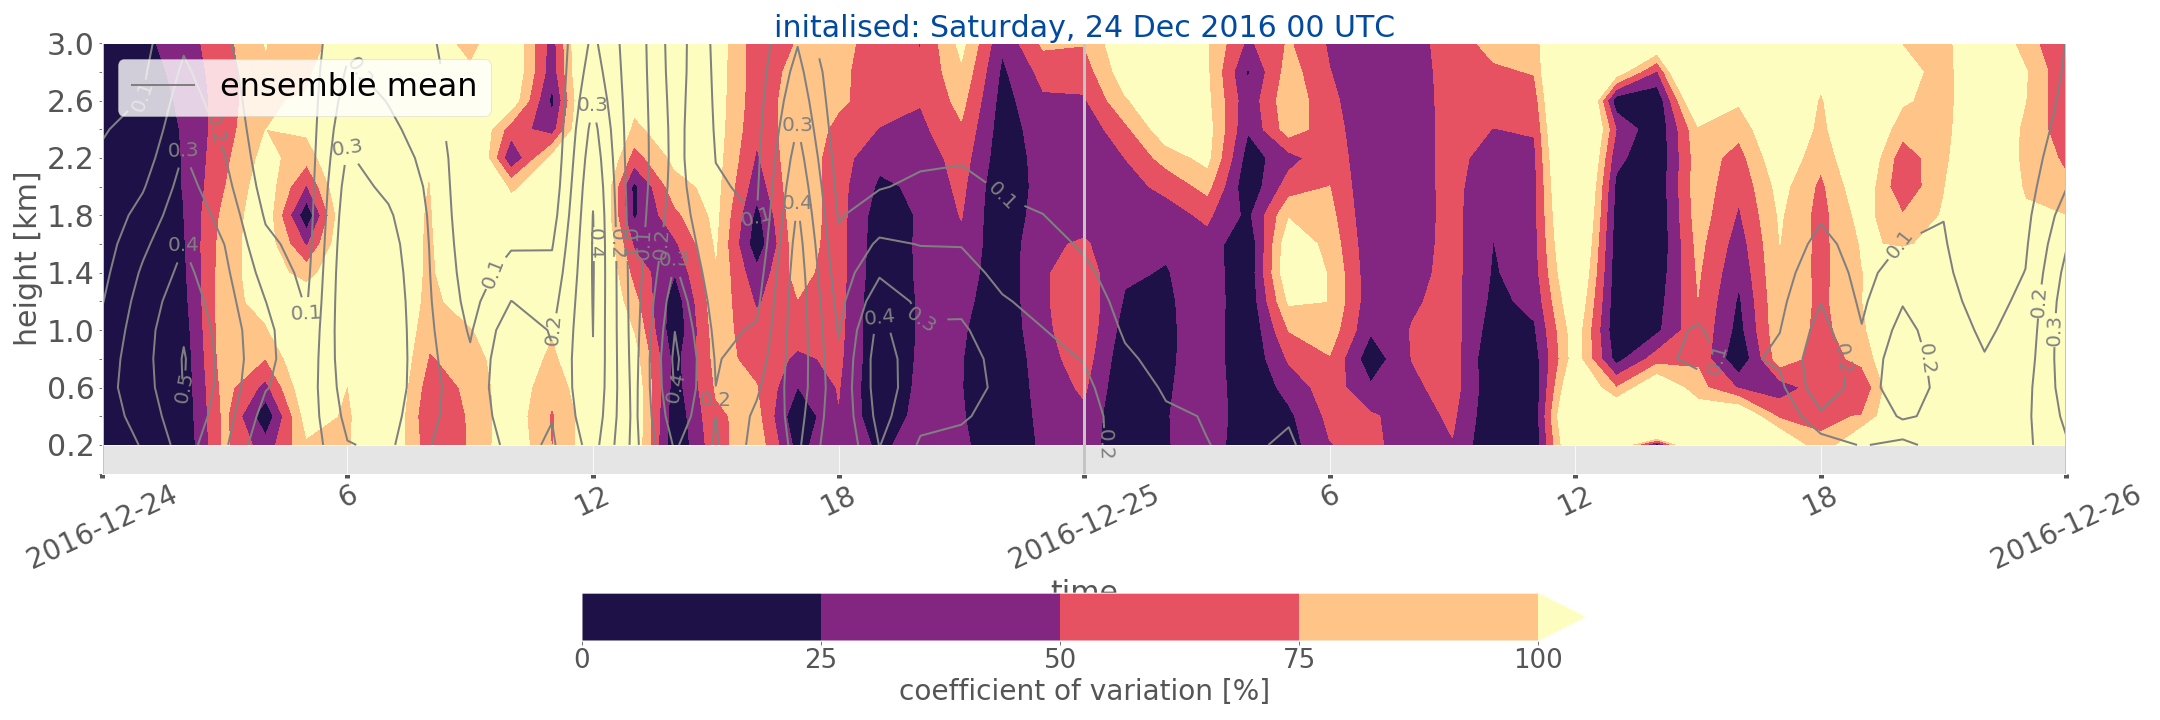
\includegraphics[trim={15.cm 0cm 15cm 21cm},clip,width=\textwidth]{./fig_variation/20161224}
		\end{subfigure}
\end{figure}
\begin{figure}[t]\ContinuedFloat
    % 22/12
		\begin{subfigure}[t]{\textwidth}		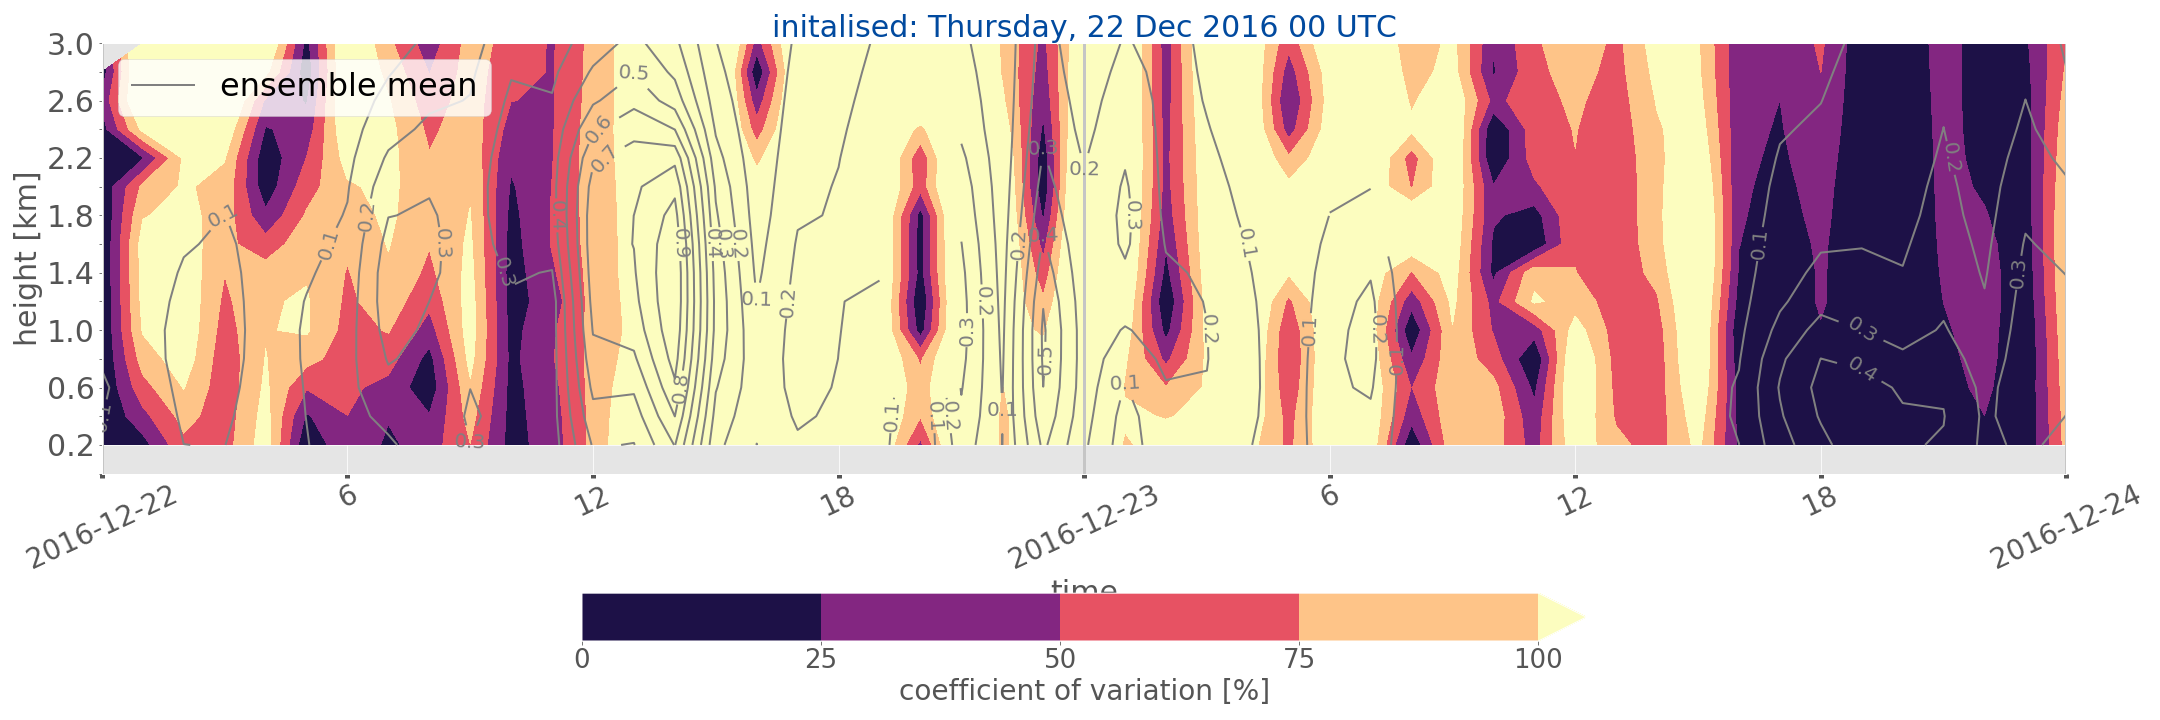
\includegraphics[trim={0.cm 5.3cm 0cm 0cm},clip,width=\textwidth]{./fig_variation/20161222}
			\caption{}\label{fig:ens_vari22}
		\end{subfigure}
    % 23/12
% 		\begin{subfigure}[t]{\textwidth}		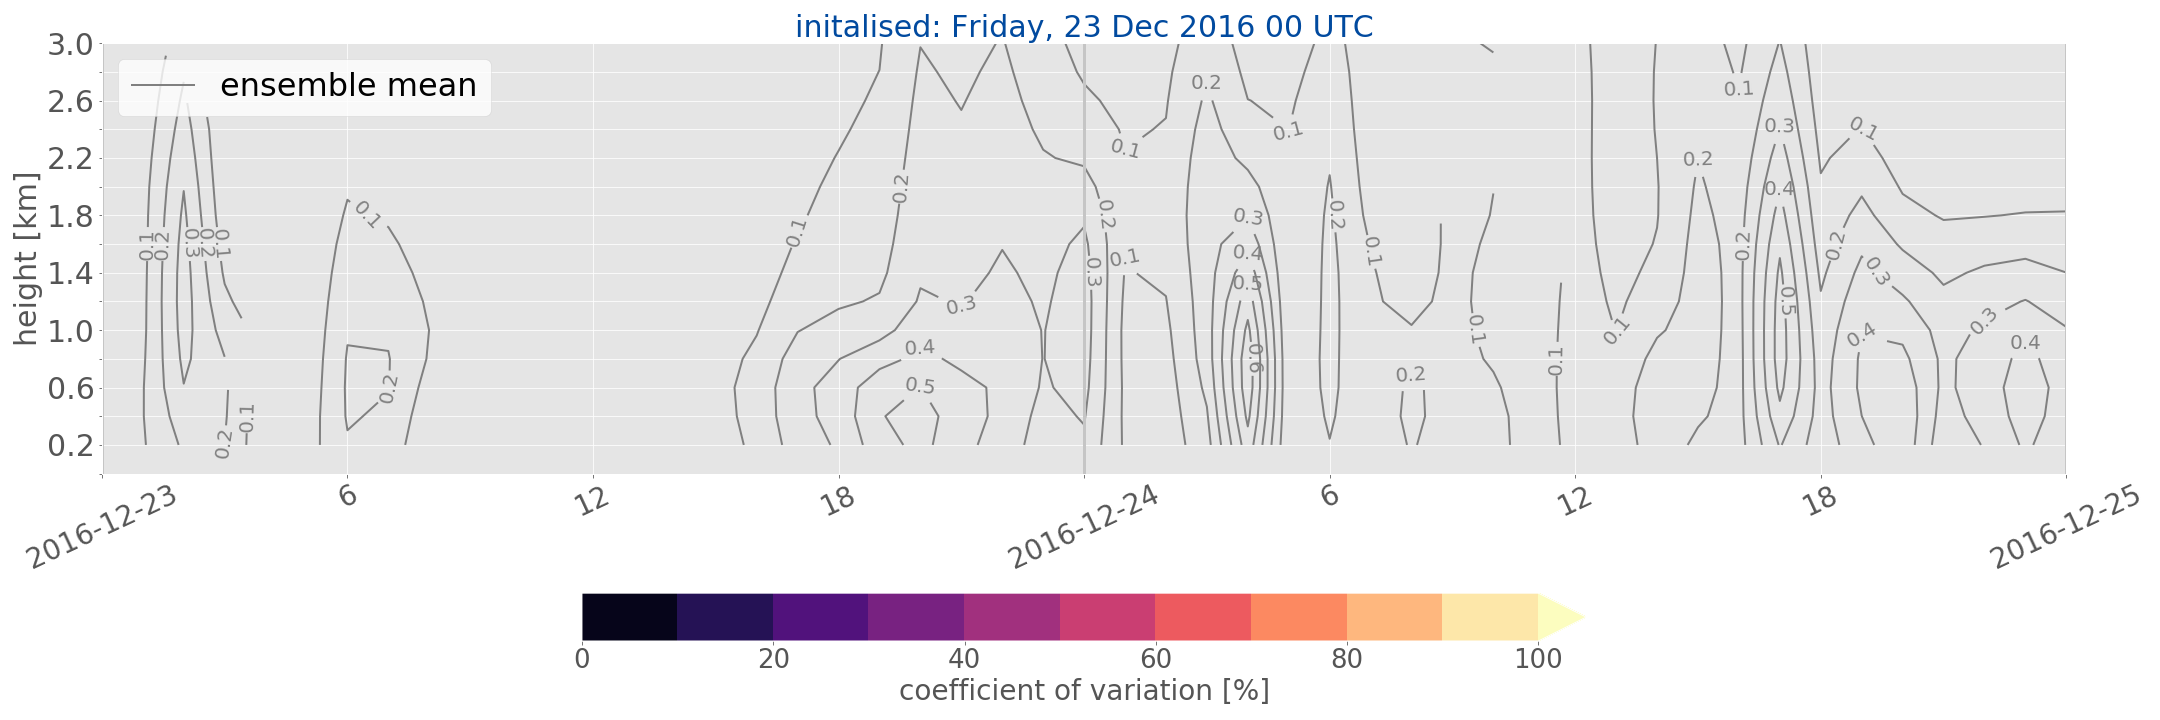
\includegraphics[trim={0.cm 0cm 0cm 0cm},clip,width=\textwidth]{./fig_variation/20161223}
% 			\caption{}\label{fig:ens_vari23}
% 		\end{subfigure}
    % 24/12
		\begin{subfigure}[t]{\textwidth}		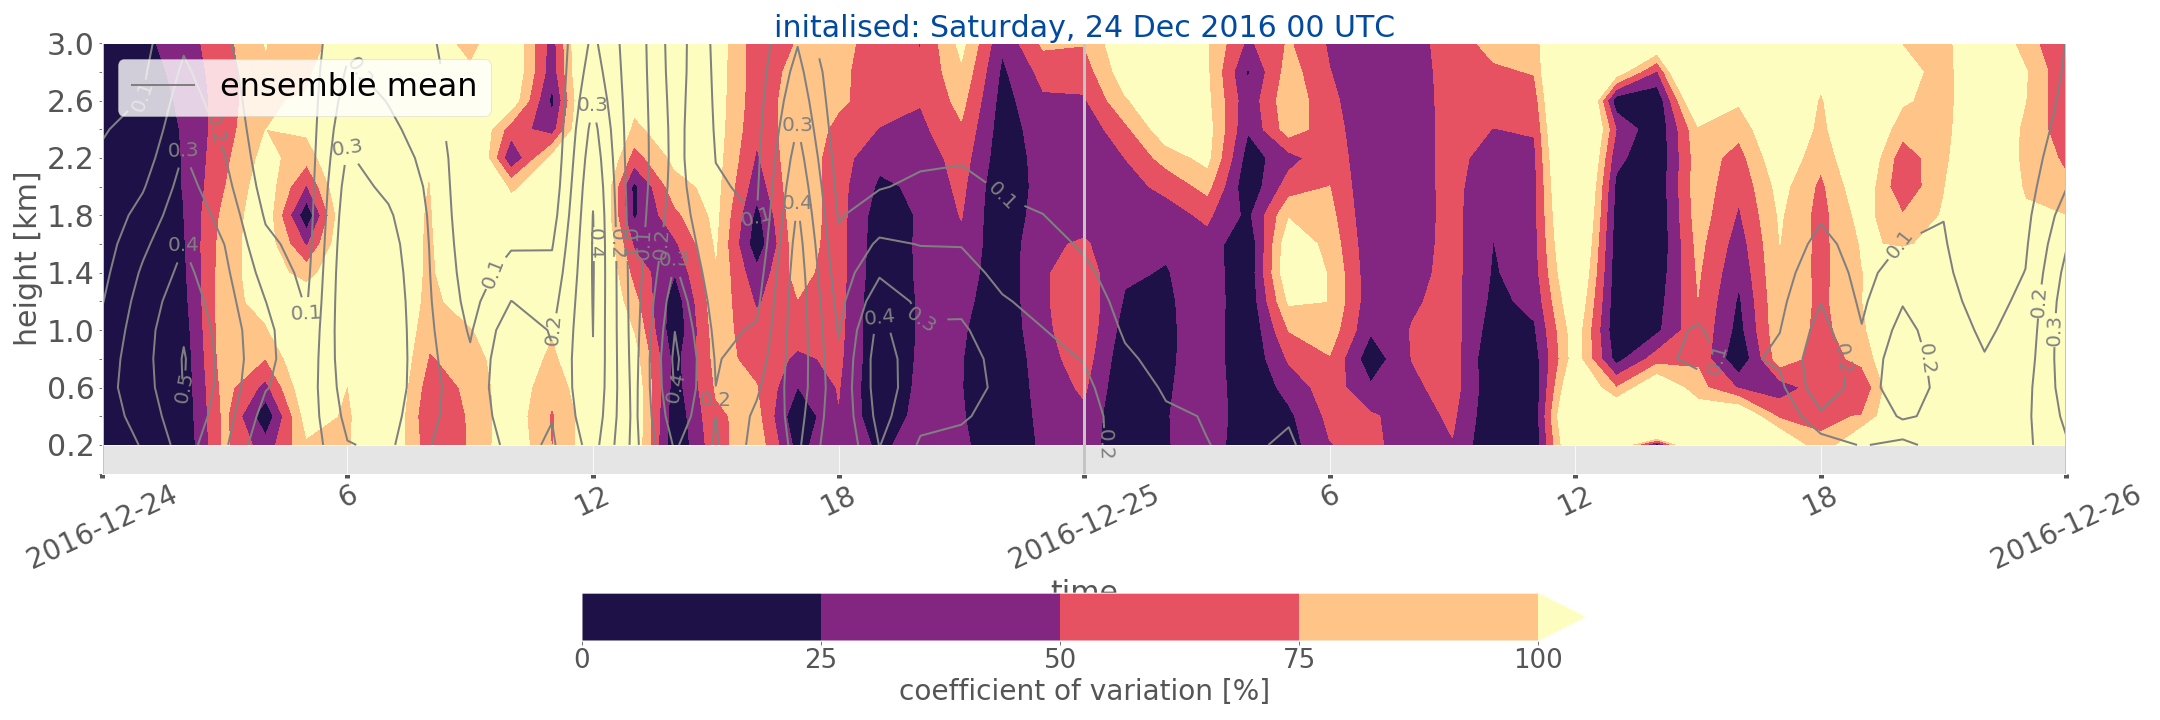
\includegraphics[trim={0.cm 5.3cm 0cm 0cm},clip,width=\textwidth]{./fig_variation/20161224}
			\caption{}\label{fig:ens_vari24}
		\end{subfigure}
        
     % colourbar
     	\begin{subfigure}[t]{\textwidth}		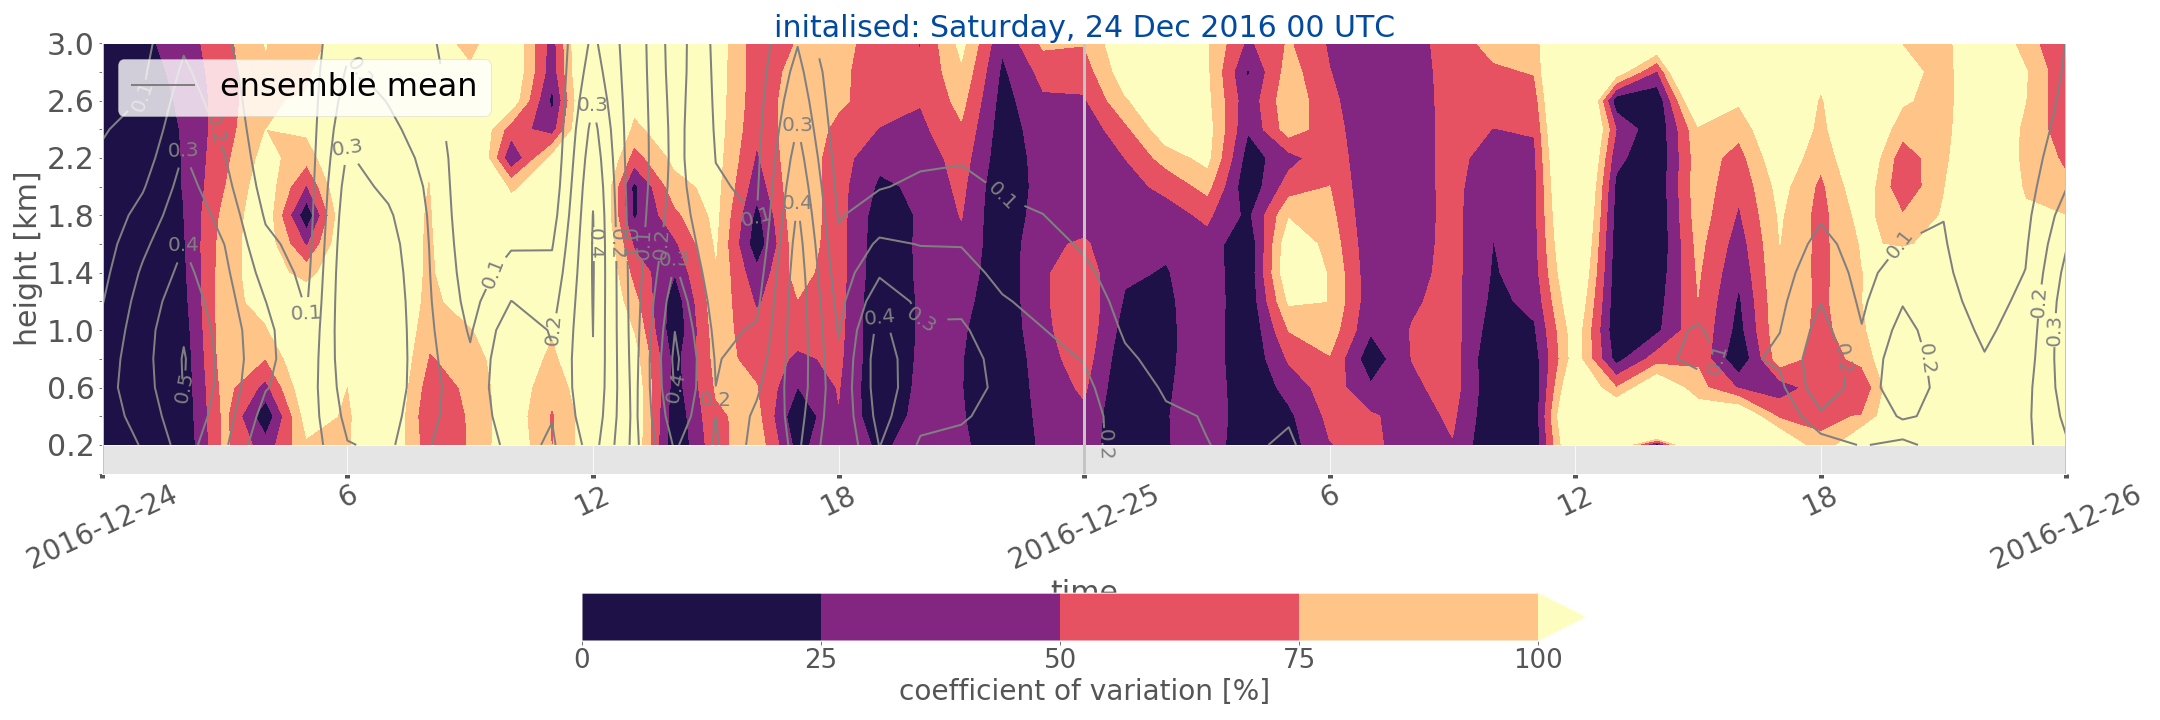
\includegraphics[trim={15.cm 0cm 15cm 21cm},clip,width=\textwidth]{./fig_variation/20161224}
		\end{subfigure}
\end{figure}
\begin{figure}[t]\ContinuedFloat
	\centering
    % 25/12
		\begin{subfigure}[t]{\textwidth}		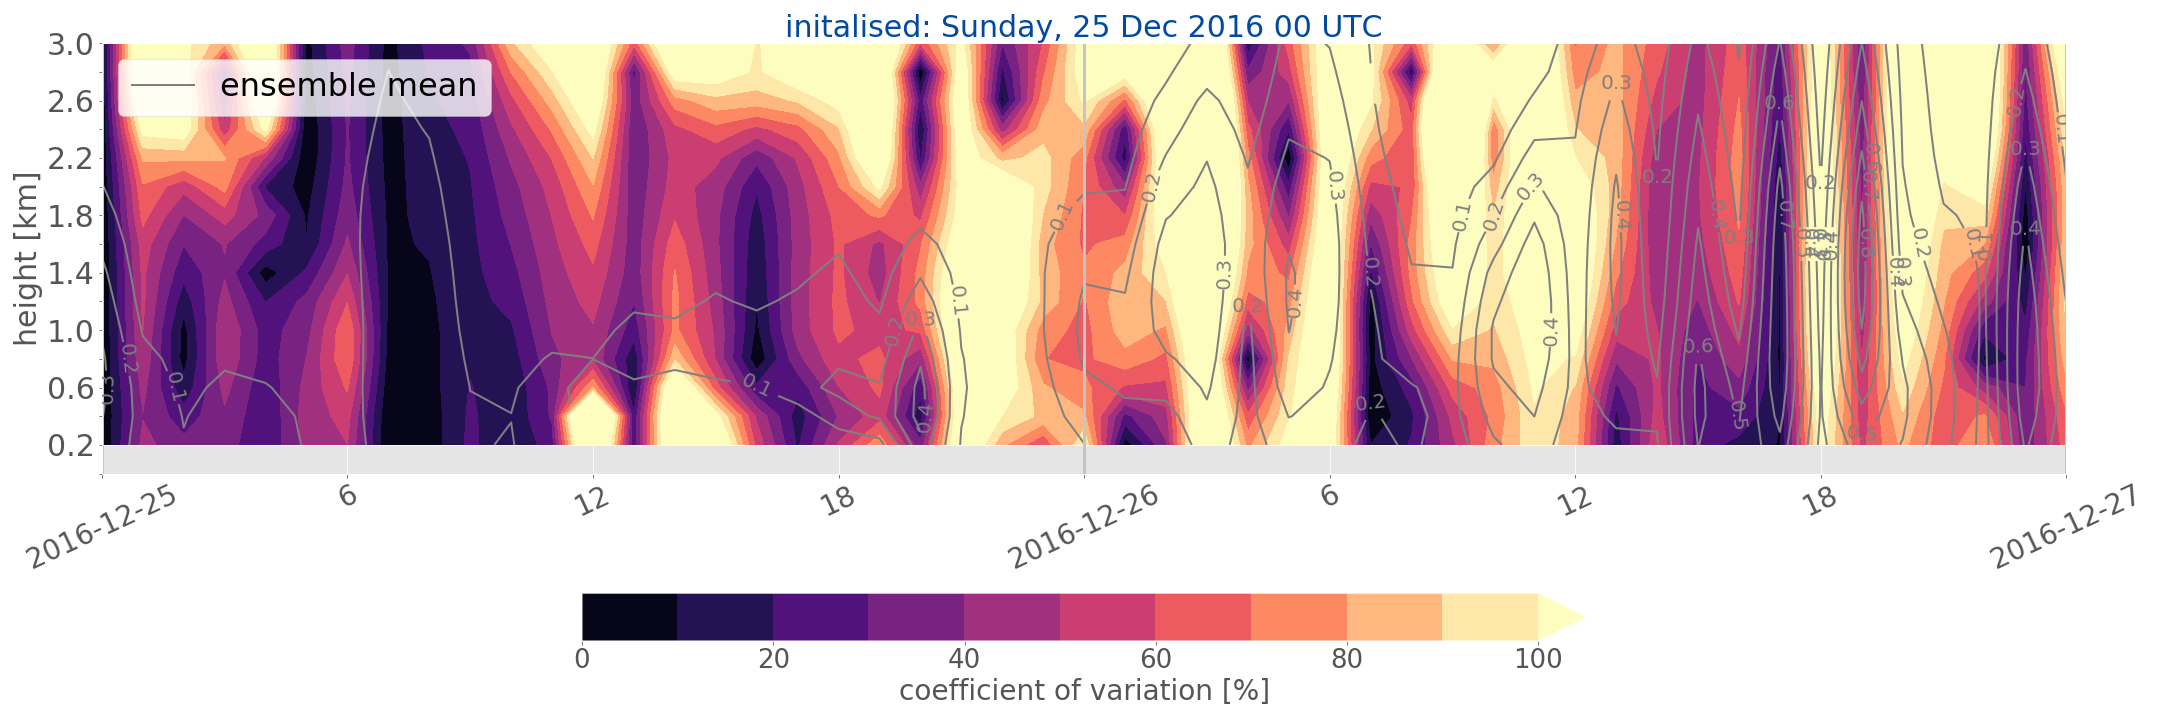
\includegraphics[trim={0.cm 5.3cm 0cm 0cm},clip,width=\textwidth]{./fig_variation/20161225}
			\caption{}\label{fig:ens_vari25}
		\end{subfigure}
    % 26/12
		\begin{subfigure}[t]{\textwidth}		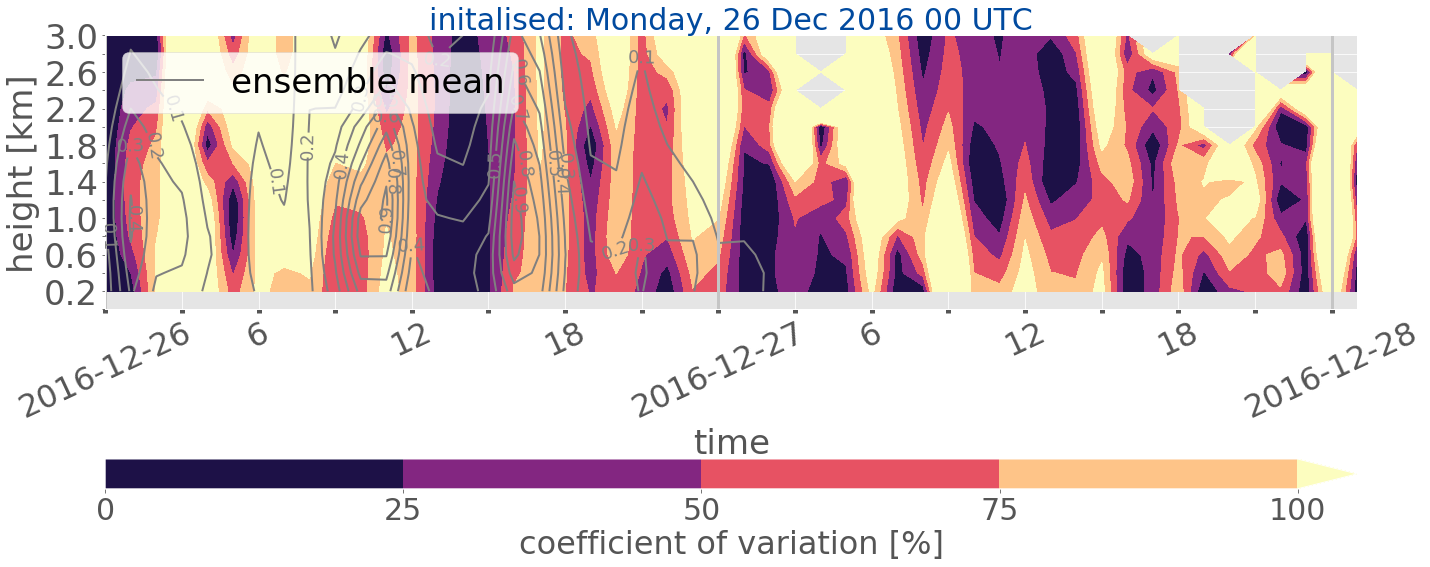
\includegraphics[trim={0.cm 5.3cm 0cm 0cm},clip,width=\textwidth]{./fig_variation/20161226}
			\caption{}\label{fig:ens_vari26}
		\end{subfigure}
%     % 27/12
% 		\begin{subfigure}[t]{\textwidth}		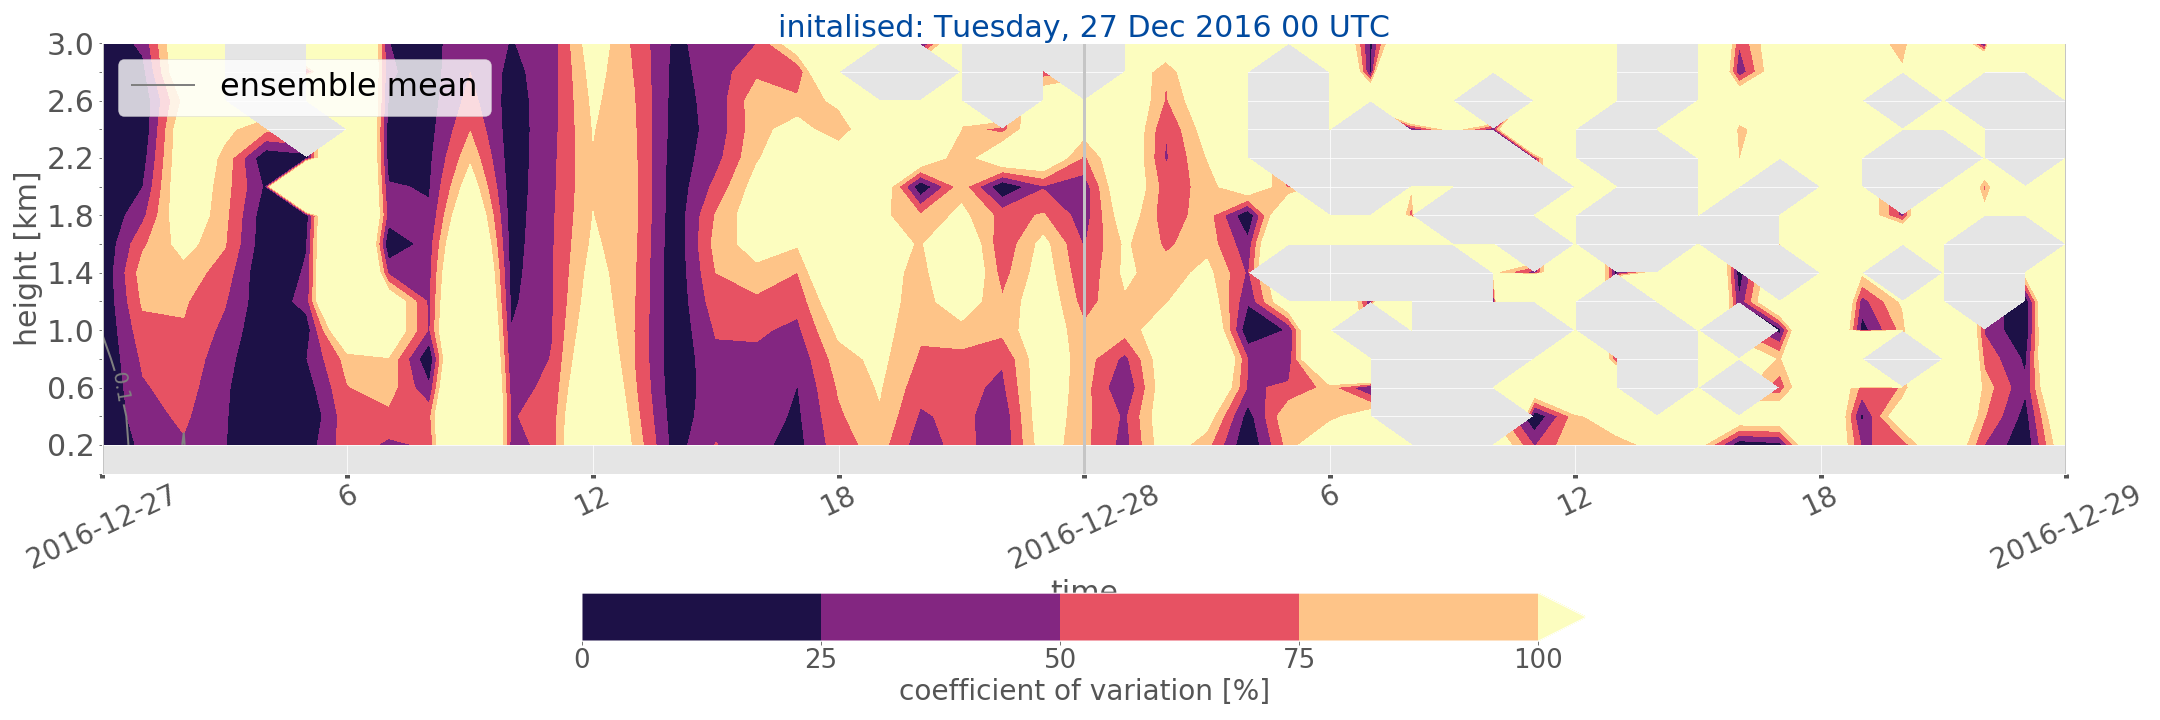
\includegraphics[trim={0.cm 5.3cm 0cm 0cm},clip,width=\textwidth]{./fig_variation/20161227}
% 			\caption{}\label{fig:ens_spread27}
% 		\end{subfigure}
        
    % colourbar
     	\begin{subfigure}[t]{\textwidth}		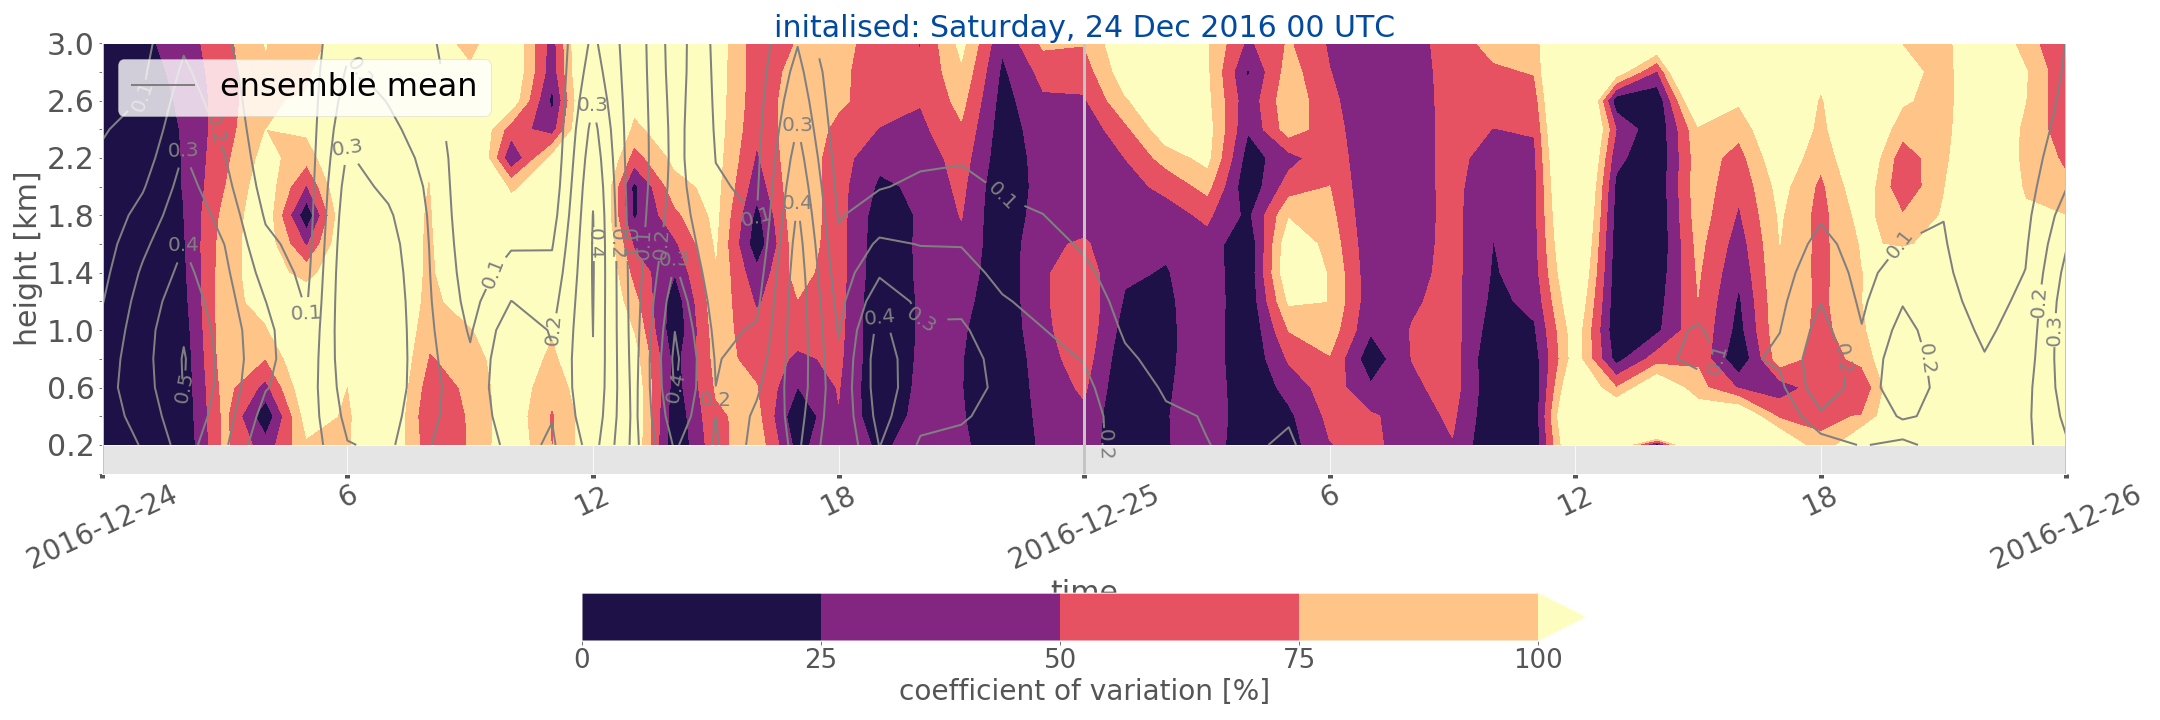
\includegraphics[trim={15.cm 0cm 15cm 21cm},clip,width=\textwidth]{./fig_variation/20161224}
		\end{subfigure}
        \caption{SWC variation of the ten ensemble members of MEPS. The lighter the colour according to the colourbar the higher the variation between the perturbed ensemble members. In grey the ensemble mean of all ten members.}\label{fig:ens_vari}
\end{figure}


%%%%%%%%%%%%%%%%%%%%%%%%%%%%%%%%%%%%%%%%%%%%%%%%%%%%%%%%%%%%%%%%%%%%%%%%%%
To verify how well the ensemble forecast system MEPS has performed, a verification is performed as described in \Cref{sec:ens_mean_spread}. \Cref{fig:ens_vari20,fig:ens_vari21,fig:ens_vari22,fig:ens_vari24,fig:ens_vari25,fig:ens_vari26} show the coefficient of variation for SWC, which is the standard deviation of the ten ensemble members divided by the mean of all ensemble members. This coefficient gives the possibility to compare the SWC results for different days with different values. It also shows if the ensemble spread (standard deviation of all ensemble members) is low the SWC is does not need to be less variable.
%\\
% %%% table verification %%%%%%%%%%%%%%%%%%%%%%%%%%%%%%%%%%%%%
\begin{table}[t!]
	\begin{center}
		\caption{Interpretation of the coefficient of variation for SWC.} \label{tab:verification}
		\begin{tabular}{lc|c|c}
			\hline\hline
			\multicolumn{2}{c|}{\textbf{Size of CV}} & \multicolumn{2}{c}{\textbf{Interpretation}} \\ 
			\multicolumn{2}{c|}{[\SI{}{\percent}]} & variability & forecast accuracy \\ \hline \hline 
			\multicolumn{2}{c|}{\numrange{0}{< 25}} & negligible & very high  \\ \hline
			\multicolumn{2}{c|}{\numrange{25}{< 50}} & low & high \\ \hline
			\multicolumn{2}{c|}{\numrange{50}{< 75}} & moderate & moderate \\ \hline
			\multicolumn{2}{c|}{\numrange{75}{< 100}} & high & low \\ \hline
			\multicolumn{2}{c|}{\num{100} to $\infty$} & very high & no  \\ \hline \hline
		\end{tabular}
	\end{center}
\end{table}
%%%%%%%%%%%%%%%%%%%%%%%%%%%%%%%%%%%%%%%%%%%%%%%%%%%%%%%%%%%%%%%%%%%%%%%%%%
% 
The grey line in \Cref{fig:ens_vari} shows the ensemble mean as a contour. The darker the colour in \Cref{fig:ens_vari} the smaller is the variation of SWC relative to the mean. The \SI{23}{\dec} does not exist, because it had too few ensemble members (only six) to create a reasonable verification and therefore is the ensemble mean in \Cref{fig:SWC23} classified as very uncertain. The interpretation of the coefficient of variation for SWC is presented in \Cref{tab:verification}.
\\
A small CV indicates a very high forecast accuracy, since the variability is negligible between the ten ensemble members (\SIrange{0}{< 25}{\percent}). Similar is a large CV associated with a low forecast accuracy and therefore a very high variability between the members (\SI{> 100}{\percent}). As expected increases the forecast uncertainty with increasing prediction time. It is still possible that in some cases the CV will be larger with a shorter prediction time than with a longer lead time. This could be the case, when strong synoptic systems with complex structure are apparent.
\\
In some cases increases the forecast accuracy with lead time. It also shows, that the CV agrees well with the prediction of the up-slope events and is more often uncertain about the pulsing part, when west wind is observed. 
\\
\\
The \SI{21}{\dec} contained an up-slope event between \SIrange{9}{13}{\UTC} and a wind change to west followed a pulsed precipitation afterwards. The coefficient of variation of the SWC in \Cref{fig:ens_vari20} shows a variation of up to \SI{100}{\percent} for the up-slope and more than \SI{100}{\percent} for the pulsed part, when initialised on \SI{20}{\dec}. An initialisation on \SI{21}{\dec} gives a better result, were the variation is less with a pronounced accuracy of up to \SI{30}{\percent} for the up-slope part around noon. 
The variation shows another good agreement around \SI{19}{\UTC}, one hour prior the maximum predicted mean SWC. For the maximum observed SWC is the CV higher than \SI{90}{\percent} and thus no forecast accuracy exists. This maximum followed from the fact, that the deterministic forecast is the strongest at time and all other ensemble members respond with a weaker SWC. The very high variability and the discrepancy between the ensemble members will be discussed further in \Cref{sec:vertEM09:2112}.
\\
While the ensemble mean produced a high SWC at \SIlist{11;14}{\UTC} on the \SI{22}{\dec}, shows the variation of SWC a very high variability at this times, when initialised on \SI{21}{\dec} (\Cref{fig:ens_vari21}). This follows a high uncertainty of the SWC peak values in \Cref{fig:SWC21}, whereas it is very certain some hours before when almost no snow water content was present. 
For an initialisation on \SI{22}{\dec} is the peak around \SI{11}{\UTC} merged together with the one at \SI{14}{\UTC}. The CV in \Cref{fig:ens_vari22} displays again a very high forecast accuracy (\SI{< 25}{\percent}) for little SWC and very high variability when the SWC peaks were observed. A moderate to low forecast accuracy can be seen around \SI{3}{\UTC} when the SWC is not higher than \SI{0.3}{\SWC}. 
A reason for this discrepancy is again due to the very high predicted SWC performed by the first ensemble member (\Cref{fig:EM09_22}). Here it shows, that six ensemble members would predict a high SWC around noon, which almost agrees with the vertical retrieved SWC. The pulsing after \SI{18}{\UTC} is forecasted by the first ensemble member and the forth, fifth, and seventh show a possibility of precipitation as well. 
According to the CV in \Cref{fig:ens_vari21} and \ref{fig:ens_vari22} exists there no forecast accuracy for the predicted peaks and the forecasts are only reliable when there is almost no SWC predicted. On \SI{22}{\dec} shows the forecast for initialisations more than \SI{24}{\hour} and less than \SI{24}{\hour} prior a pattern as for few precipitation is the forecast accuracy high to very high and for higher SWC is the forecast accuracy not existing. 
\\
All ensemble members agree well with the occurrence of the up-slope storm on \SI{23}{\dec} (\Cref{fig:EM09_22}). The verification in \Cref{fig:ens_vari22} shows little discrepancy below \SI{50}{\percent} with most having a high forecast accuracy. All ten ensemble members forecast the up-slope to occur after \SI{16}{\UTC}, compare \Cref{fig:EM09_22}. While comparing only six ensemble members in \Cref{fig:EM09_23}, one could assume that the uncertainty of all ensemble members during the up-slope storm is low, but not as certain as for an initialisation on \SI{22}{\dec} at \SI{0}{\UTC}. 
The deterministic forecast (EM0) and ensemble member one in \Cref{fig:EM09_22} indicate peaks of high SWC before \SI{8}{\UTC}. The retrieved SWC on \SI{23}{\dec} had two peaks, one at around \SI{2}{\UTC} and another at \SI{4}{\UTC}. The deterministic forecast, initialised on \SI{22}{\dec} predicted a peak at \SIlist{2;6;8}{\UTC}, where the first ensemble member (EM1) has a strong SWC at \SI{7}{\UTC}. Overall seems a combination of the deterministic and first ensemble member of the  \SI{22}{\dec} initialisation to be a good forecast when comparing to the retrieved SWC in \Cref{fig:SWC22}.
\\
The \SI{24}{\dec} was one of the days, where pulsing of the storm was observed and predicted throughout the day. 
\Cref{fig:EM09_23} can give an idea about the variation between the six existing forecasts. Three ensemble members (EM0, EM7, EM8) seem to agree on the occurrence of a SWC peak around \SI{18}{\UTC}, which would be in the range of a moderate forecast accuracy. 
For an initialisation on \SI{24}{\dec} indicates the variation coefficient of all ten ensemble members in \Cref{fig:ens_vari24} different accuracies. The ensemble mean is presented in grey and shows the pulses forecasted. Until noon on \SI{24}{\dec} is no forecast accuracy for the peaks. The peak observed at \SI{14}{\UTC} indicates a low variability between the ensemble members. The peak at \SI{17}{\UTC} has a high accuracy up to \SI{0.8}{\km} and moderate up to \SI{1.2}{\km}. After \SI{19}{\hour} forecast time is the variability between the ensemble members negligible and all agree on the existence of precipitation.
A detail inter-comparison between the surface accumulation and the vertical snow water content is presented in \Cref{sec:vertEM09:2412}.
\\
In general was the \SI{25}{\dec} a very weak snow storm with strong liquid precipitation observed between \SIlist{12;18}{\UTC}. \Cref{fig:SWC24} and \Cref{fig:SWC25} gave a low value of predicted SWC in the course of a day. As \Cref{fig:ens_vari24} indicates is the forecast accuracy very high up to \SI{1.8}{\km} until noon, this is when liquid precipitation was measured. According to \Cref{fig:LWC24} and \ref{fig:LWC25} was the depth of the liquid layer up to \SI{0.8}{\km}. The variation coefficient has a large disagreement below \SI{0.8}{\km}, but above is the variability between the members not existing or low. Initialisation on \SI{24}{\dec} show weak peak in \Cref{fig:SWC25} at \SI{18}{\UTC}, which had a moderate forecast accuracy, were it is afterwards very high. For an initialisation on \SI{25}{\dec} is the forecast accuracy high until noon (\Cref{fig:ens_vari25}). While liquid precipitation was monitored is the accuracy in the lower layer first not existing and shortly before \SI{18}{\UTC} very high. A high agreement exists for the SWC peak at \SI{20}{\UTC} up to \SI{0.8}{\km} and decreases to be moderate above. A discussion about the precipitation change and its related forecast is given in \Cref{sec:vertEM09:2512}.
\\
Again, the \SI{26}{\dec} is only comparable until \SI{17}{\UTC} even though \Cref{fig:SWC25} would suggest a continues pulsing of the storm. The two peaks around \SI{18}{\UTC} (\Cref{fig:SWC25}) are forecasted with a very high and moderate accuracy in \Cref{fig:ens_vari25}. The SWC peaks at around \SIlist{3;5}{\UTC} show a very high variability. \Cref{fig:EM09_25} shows that four out of ten ensemble members would agree with the peaked event around \SI{5}{\UTC}. Whereas the peak at \SI{3}{\UTC} is dominated by the strong predicted SWC of the deterministic forecast, which follows the high variation in \Cref{fig:ens_vari25}. 
Initialised on \SI{26}{\dec} follows that the SWC peak at \SI{1}{\UTC} is related to a moderate forecast accuracy. Low forecast accuracy is shown for the SWC between \SIrange{9}{12}{\UTC} and the one between \SIrange{15}{18}{\UTC} has a low to moderate variability between the members.  When looking at \Cref{fig:EM09_26} might this disagreement be related to the colourful variation of the vertical predicted SWC. There seems no agreement between the different members about the incidence of the SWC peaks. The high conflict for the CV before noon is most likely related to the high SWC of the deterministic SWC. 
%
% \\ \\
% Another way to verify an ensemble prediction system is to use the ensemble spread of the SWC, which is just the standard deviation of all ten ensemble members, shown in \Cref{fig:ens_spread}. Here, lighter colours of the SWC show more deviation of the SWC around the ensemble mean and darker colours indicate that the ensemble members are close to the mean. Grey contour lines indicate the ensemble mean of the SWC to see any variations.
% \\
% As the results in \Cref{fig:ens_spread} show is the spread very low for the up-slope cases (\Cref{fig:ens_spread20,fig:ens_spread21,fig:ens_spread22,fig:ens_spread23}). This means that all ensemble members perform well when the wind is from the east. 
% \\
% The ensemble spread shows more uncertainty for the pulsing events. 
% Initialisation on \SIlist{21;22;26}{\UTC} shows more spread between the different ensemble members (lighter colour in \Cref{fig:ens_spread21}, \ref{fig:ens_spread22}, and \ref{fig:ens_spread26}), especially for the ensemble mean maximum values. On these days the maximum SWC was quite high and reached the overall ensemble mean maximum of \SI{1.24}{\SWC} on \SI{21}{\dec}.
% Fewer spread between the ensemble members is shown for the initialisation \SIlist{23;24;25}{\UTC} (\Cref{fig:ens_spread23,fig:ens_spread24,fig:ens_spread25}), when the ensemble mean never reached more than \SI{0.54}{\SWC}.

%%%%%%%%%%%%%%%%%%%%%%%%%%%%%%%%%%%%%%%%%%%%%%%%%%%%%%%%%%%%%%%%%%%%%%%%%
\subsection{Wednesday, \SI{21}{\dec}}
%%%%%%%%% vertical obs %%%%%%%%%%%%%%
%\subsection{Vertical snowfall observations}
\label{sec:vertEM09:2112}
% %%% image SWP %%%%%%%%%%%%%%%%%%%%%%%%%%%%%%%%%%%%%
\begin{figure}[h]
	\centering
	\begin{subfigure}[t]{\textwidth}
		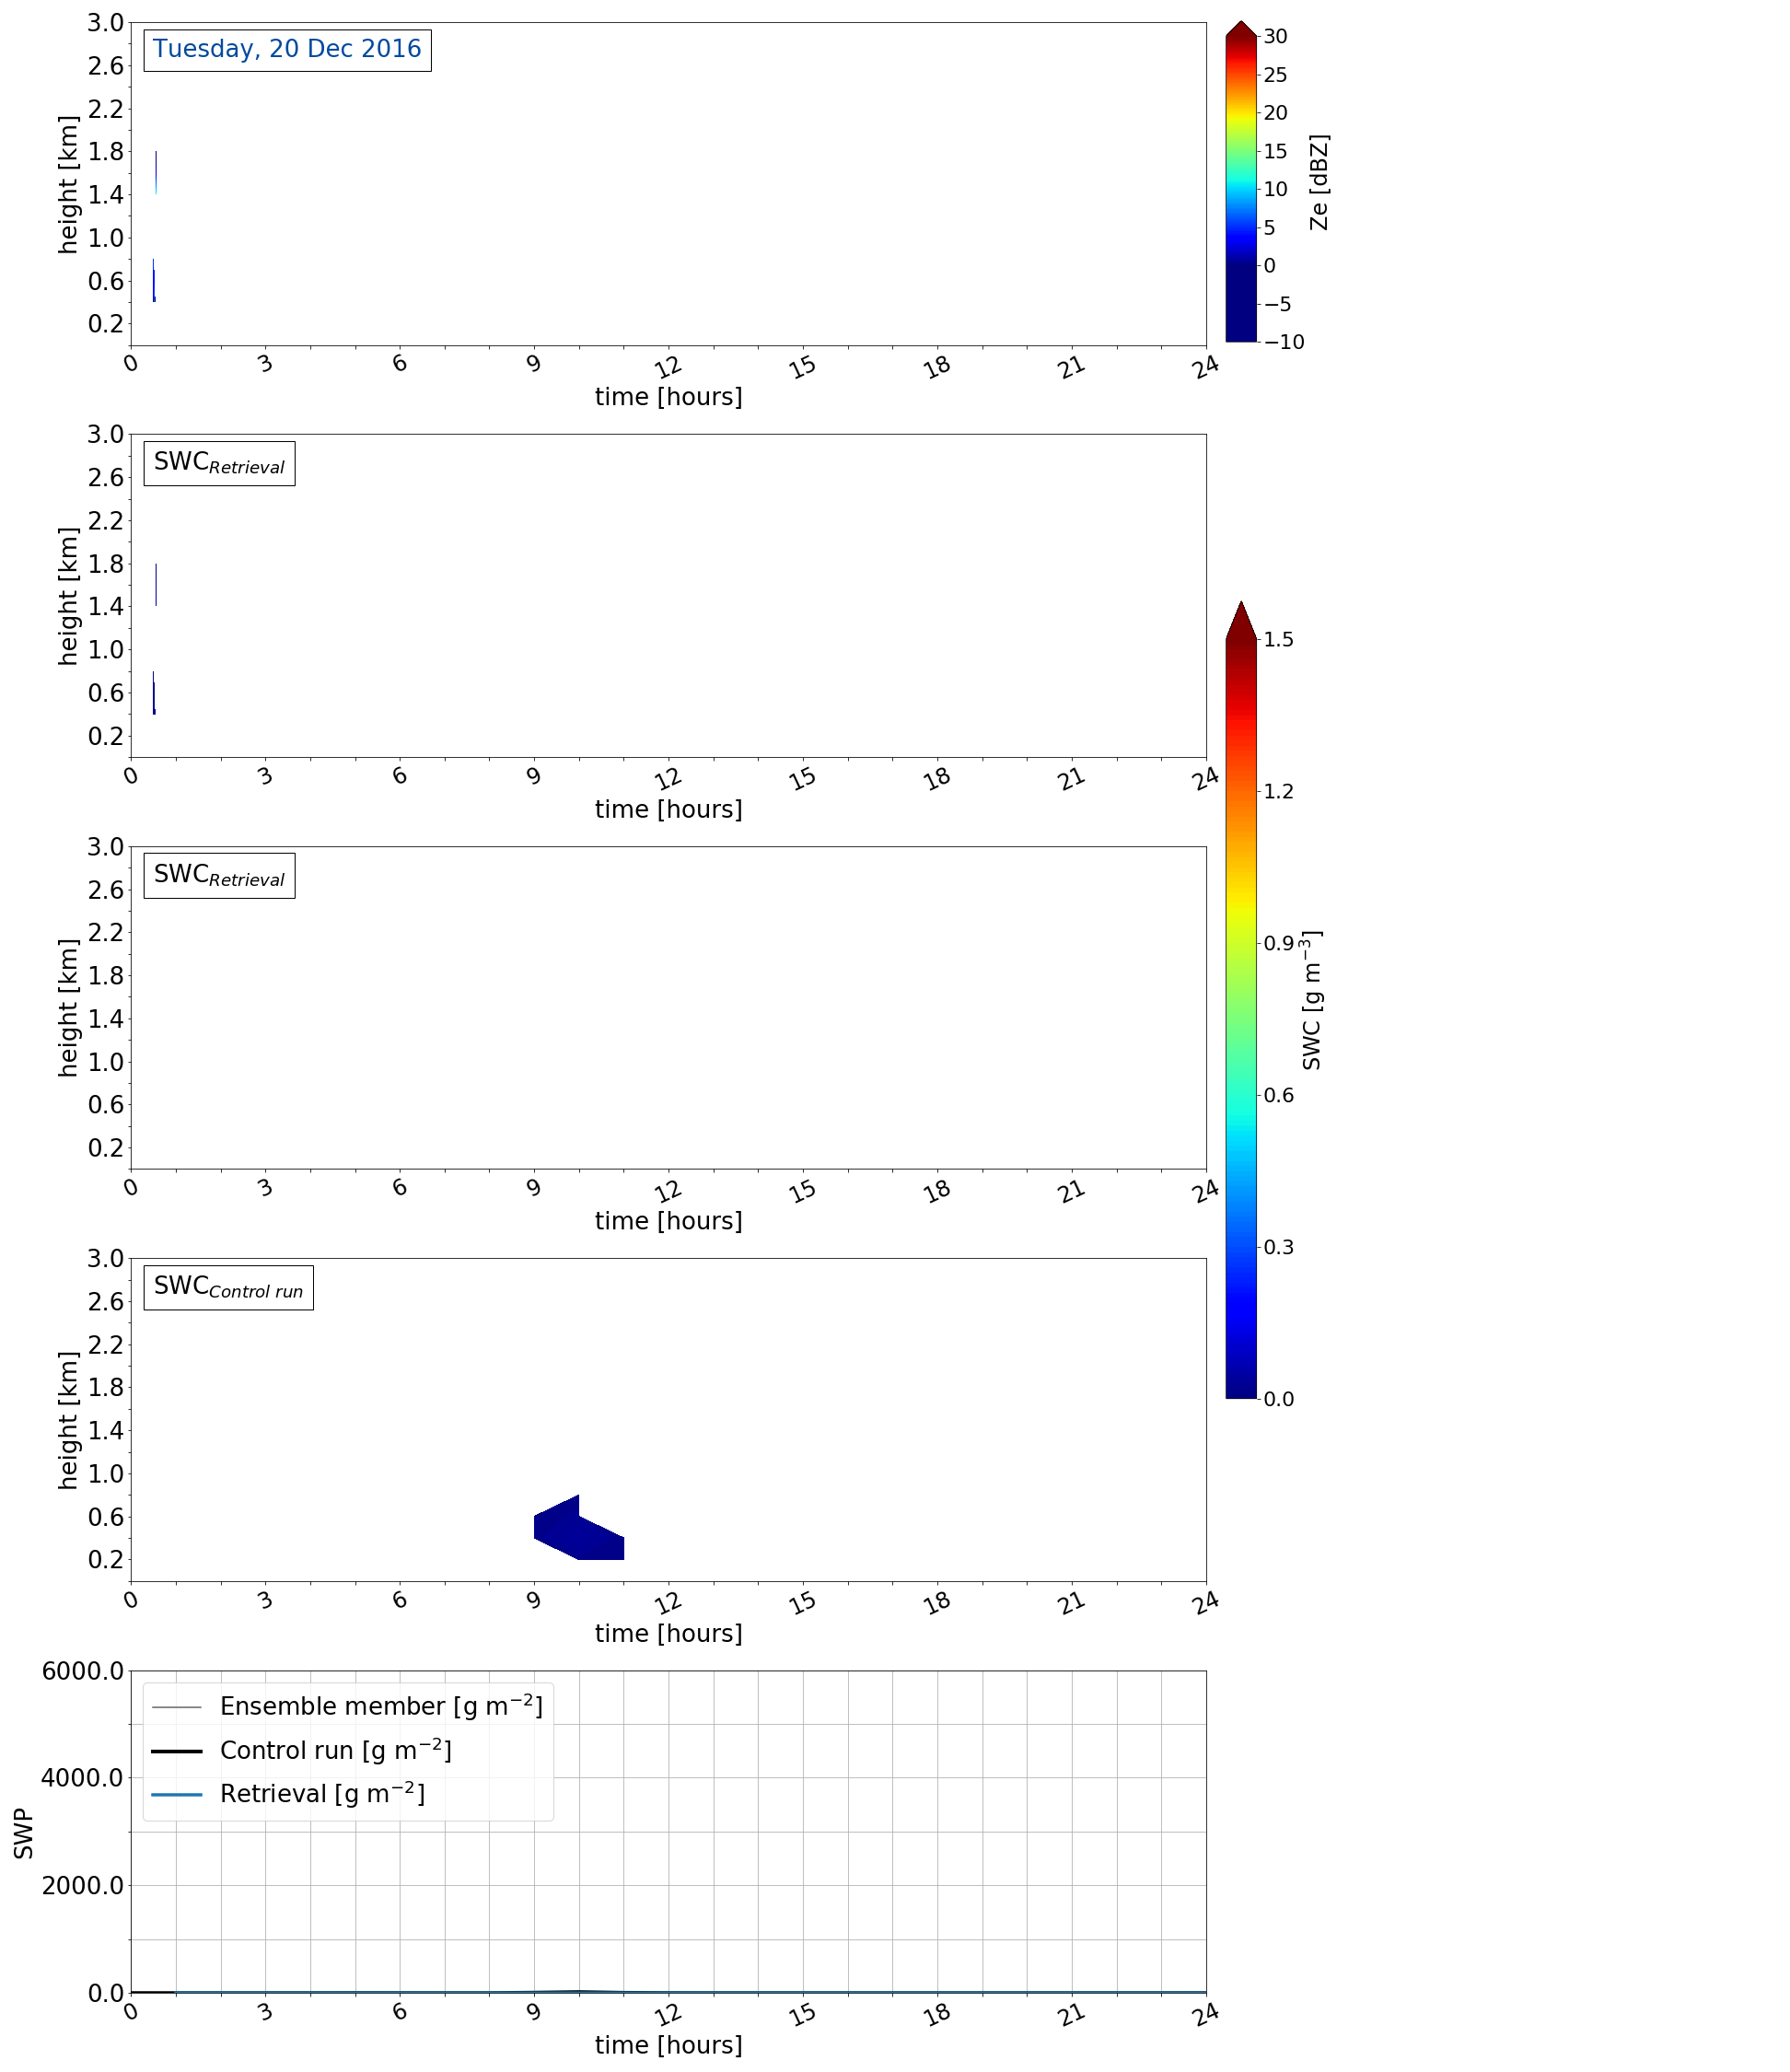
\includegraphics[trim={0.4cm .4cm 31.3cm 63.5cm},clip,width=\textwidth]{./fig_SWC/20161220}
		\caption{Initialised: Tuesday, \SI{20}{\dec}}\label{fig:SWP20}
	\end{subfigure}
	\begin{subfigure}[t]{\textwidth}
		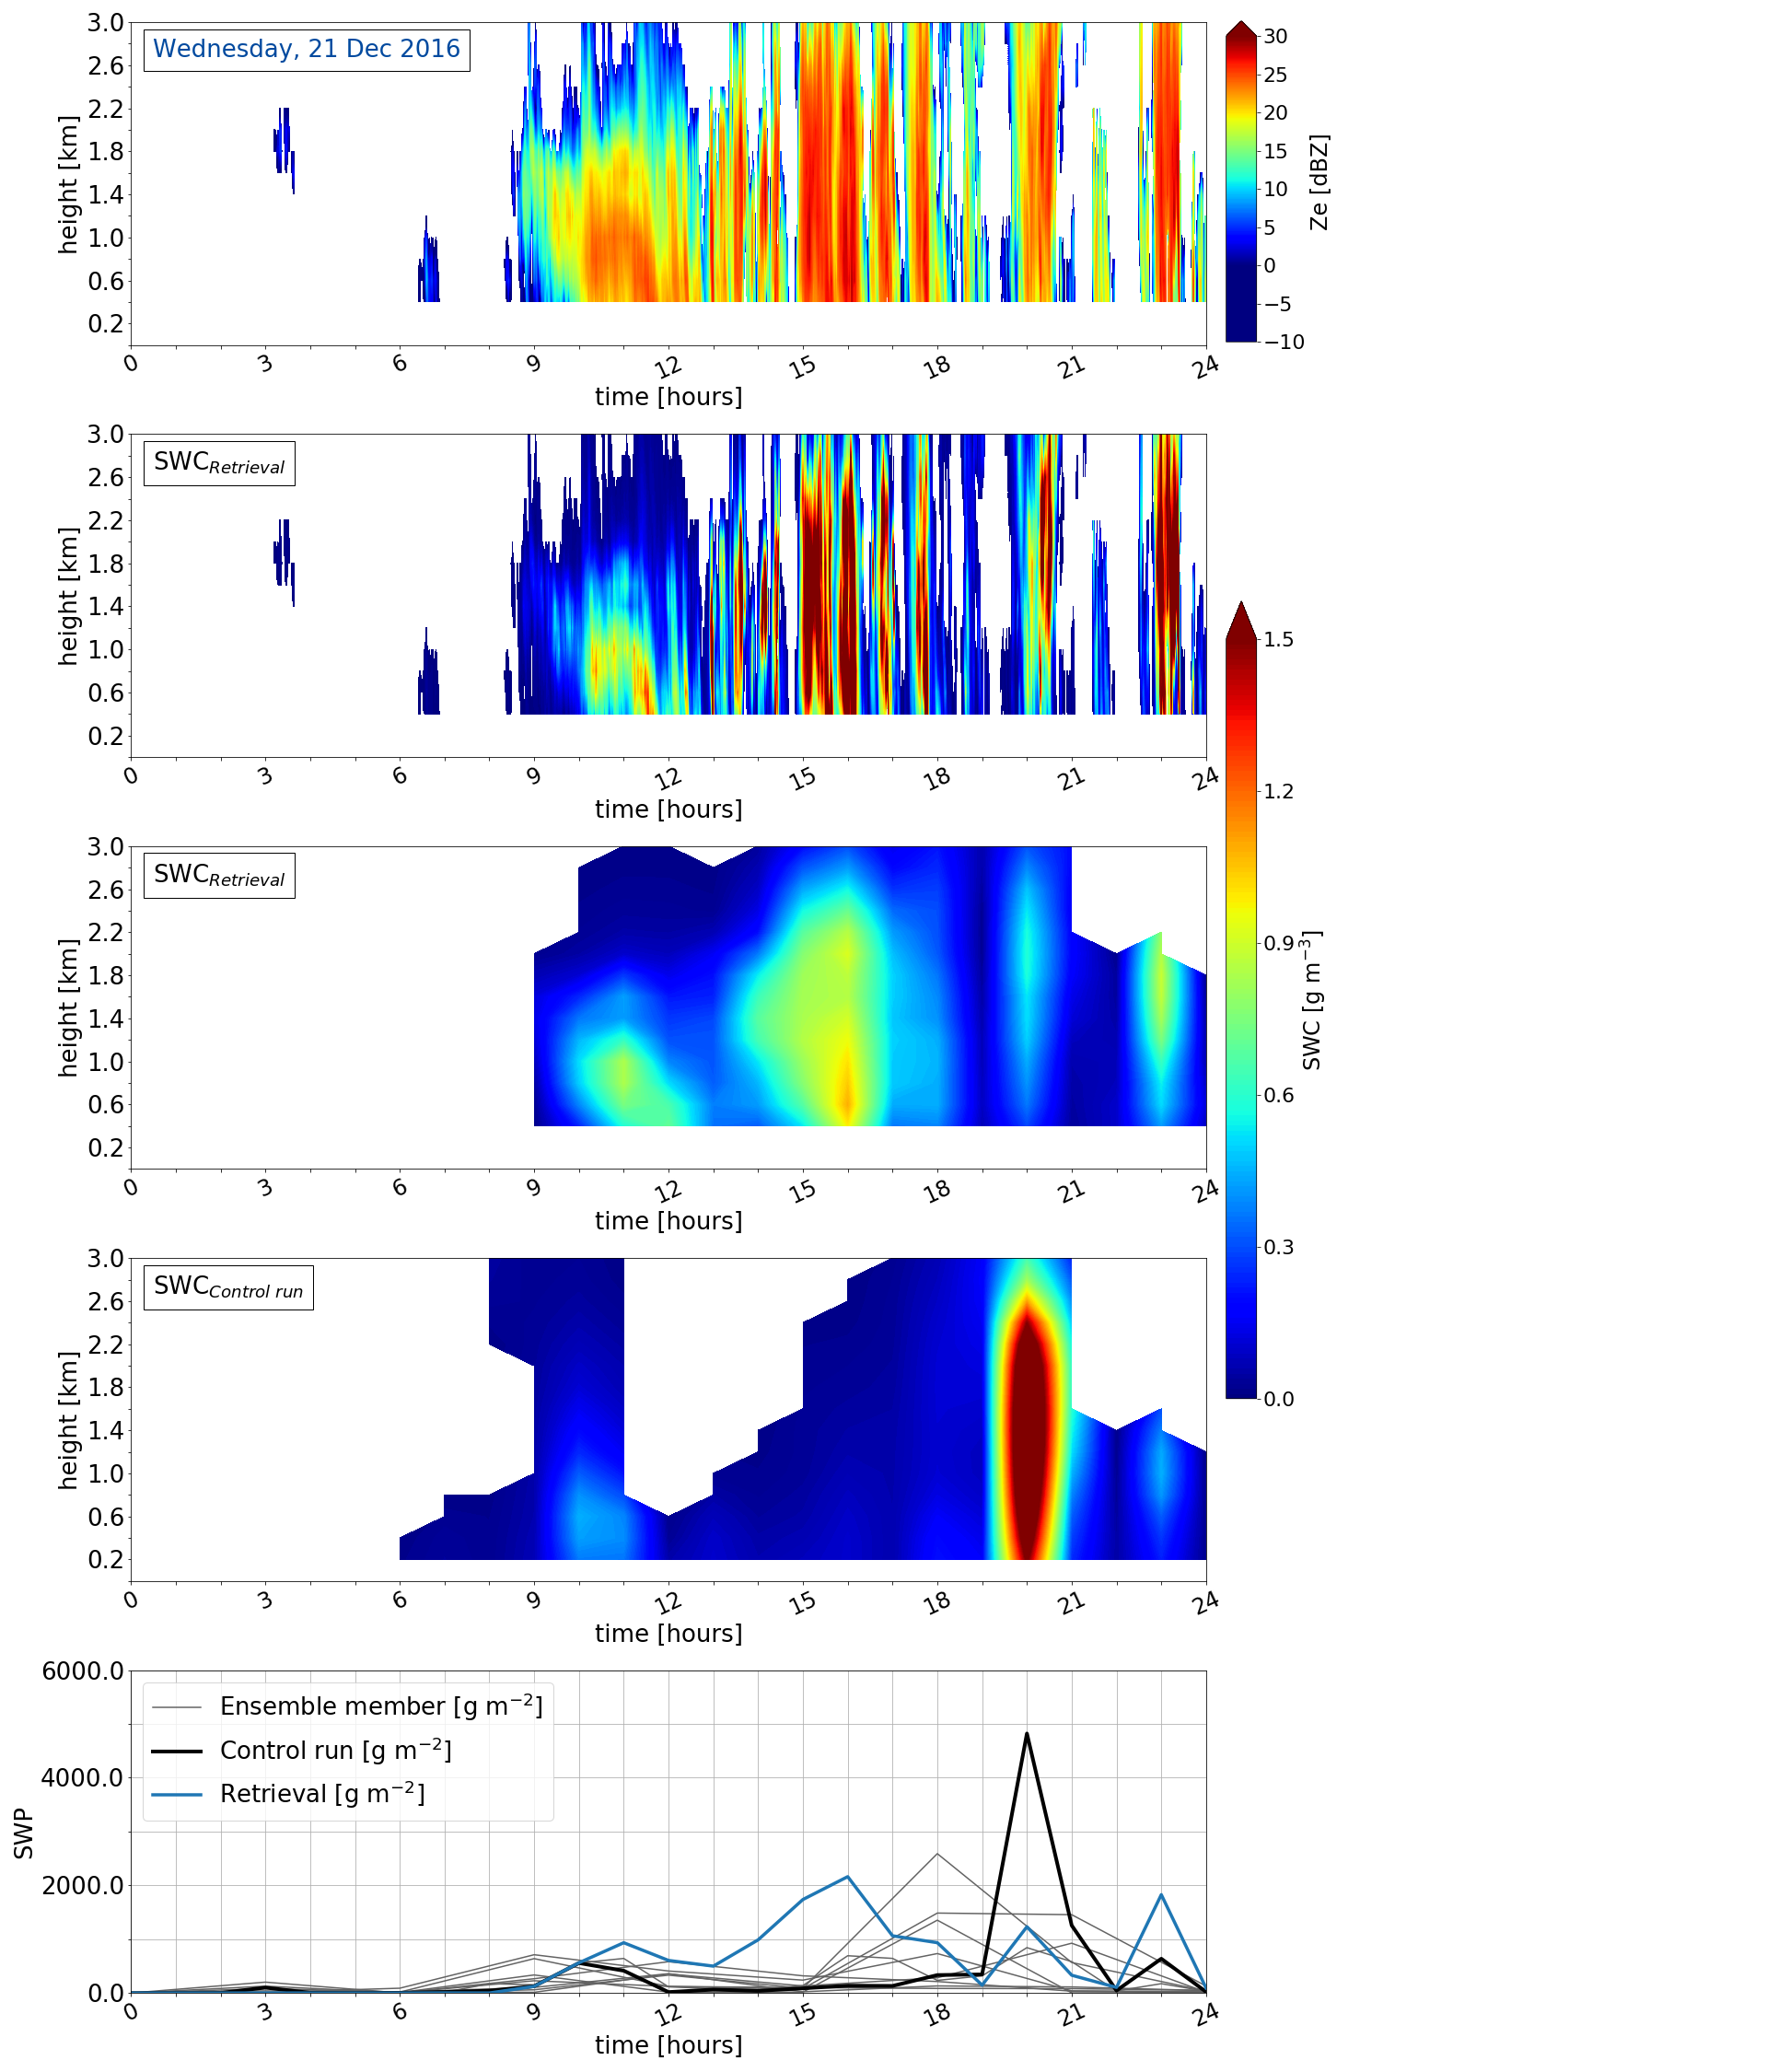
\includegraphics[trim={0.4cm .4cm 31.3cm 63.5cm},clip,width=\textwidth]{./fig_SWC/20161221}
		\caption{Initialised: Wednesday, \SI{21}{\dec}}\label{fig:SWP21}
	\end{subfigure}
	\caption{}\label{fig:SWP2021}
\end{figure}
%%%%%%%%%%%%%%%%%%%%%%%%%%%%%%%%%%%%%%%%%%%%%%%%%%%%%%%%%%%%%%%%%%%%%%%%%%
It shows from the SWP image in \Cref{fig:SWP21}, that the deterministic forecast of MEPS (black line) dominates. Most of the other ensemble members (grey line) prognoses the daily maximum snowfall amount two hours earlier than the deterministic forecast. The blue, dashed line, indicating the ensemble mean SWP shows the weakening of the snowfall amount when taking the average of all ten ensemble members with a maximum value at \SI{20}{\UTC}. By comparing the orange line (SWP from the retrieval) and the blue, dashed line it shows, that the ensemble mean value of MEPS gets closer to the observed one, \SIlist{2833; 2162}{\SWP} respectively.
%
% %%% image ensemble member 0-9 %%%%%%%%%%%%%%%%%%%%%%%%%%%%%%%%%%%%%
\begin{figure}[t]
	\centering
	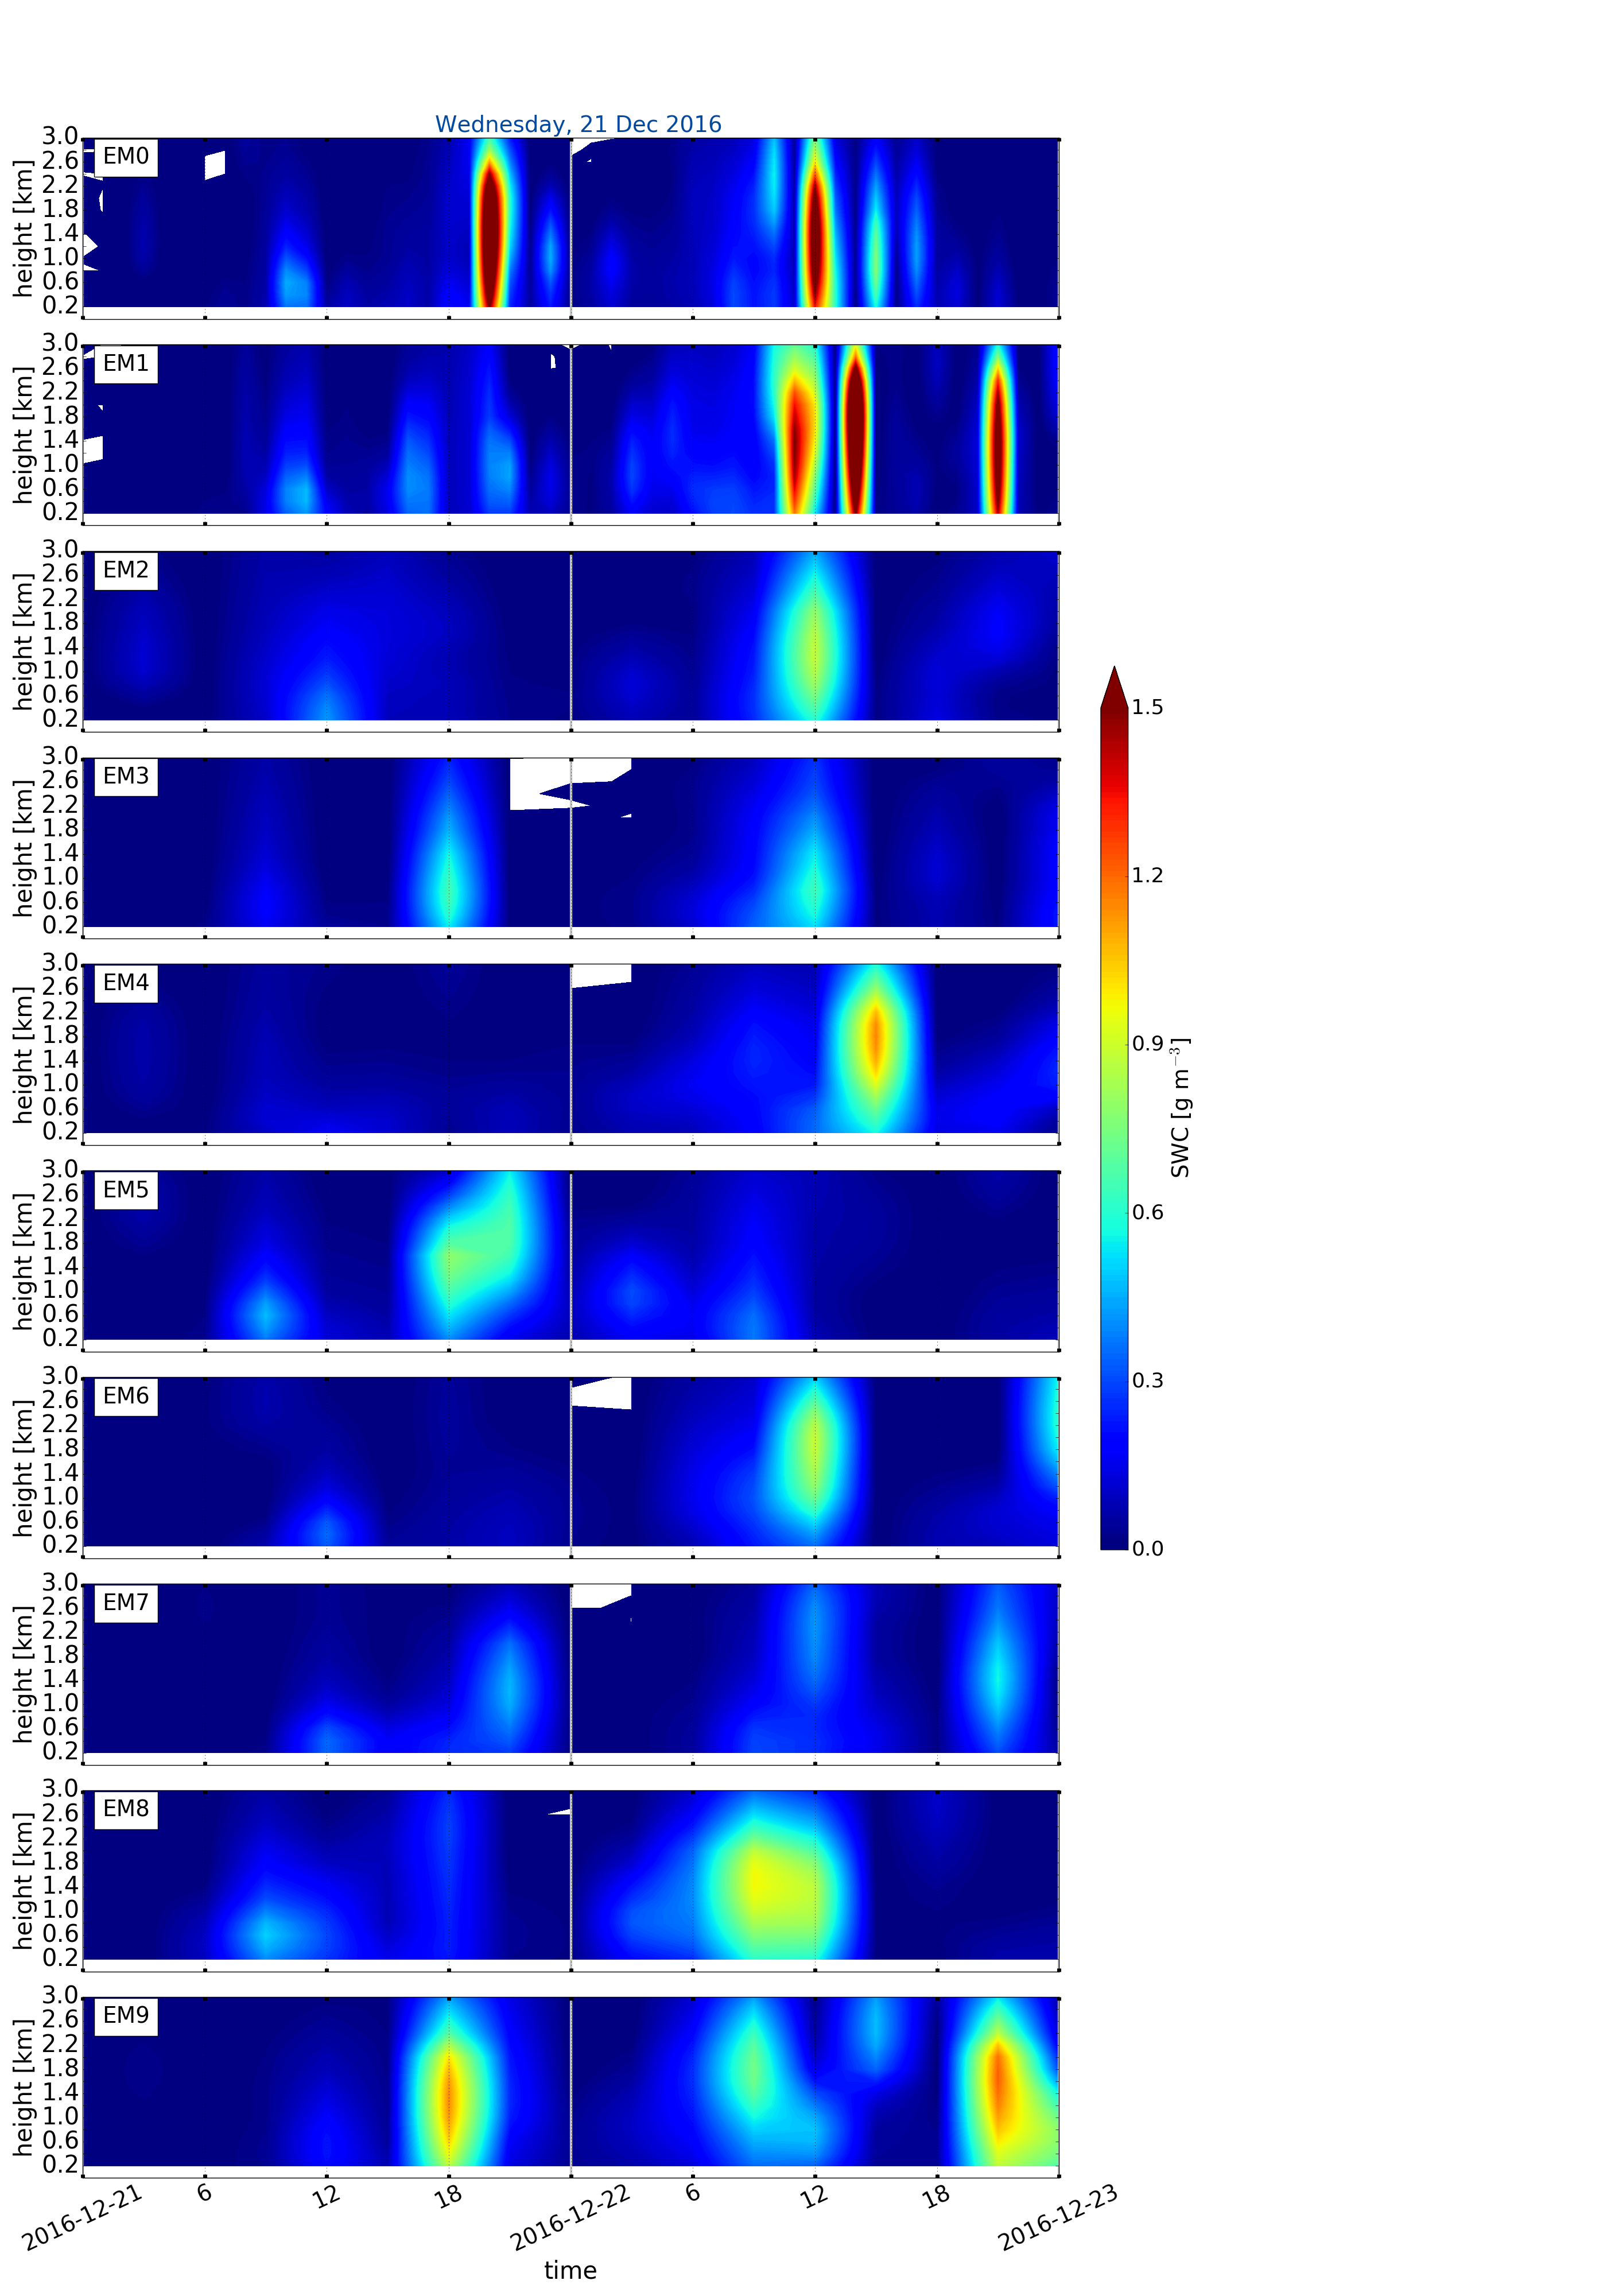
\includegraphics[trim={0cm 0cm 18.3cm 5.1cm},clip,width=0.8\textwidth]{./fig_09EM/20161221}
	\caption{SWC of all ensemble members initialised Wednesday, \SI{21}{\dec} at 0\SI{0}{\UTC} forecast for \SI{48}{\hour}.}\label{fig:EM09_21}
\end{figure}
%%%%%%%%%%%%%%%%%%%%%%%%%%%%%%%%%%%%%%%%%%%%%%%%%%%%%%%%%%%%%%%%%%%%%%%%%%
%
\textcolor{red}{DISCUSSION! Why does MEPS not catch that peak at \SI{16}{\UTC}? Maybe because it is too close to the up-slope storm. Also, Why is the control so high compared to the perturbed members? It catches the up-slope part when also a little weak. Most of the ensemble members would have caught it around \SI{9}{\UTC}. One ensemble member has predicted a high value of SWC at \SI{18}{\UTC}, compare to \Cref{fig:EM09_21}. Why is the up-slope storm more consistent compared to the pulsing? Regional effects? MEPS does well even with catching the pulses and up-slopes, at Haukeliseter is a very difficult orography. }
% %
\newline \noindent
The vertical temperature profile performed with MEPS in \Cref{fig:meps_sound_20} and \ref{fig:meps_sound_21}, shows that an initialisation \SI{36}{\hour} prior to the event would give a cloud with height up to \SI{3}{\km}, as observed in \Cref{fig:SWC21} first panel. An initialisation closer to the occurrence of the storm shows, that MEPS underestimates the intensity and height of the storm (\Cref{fig:meps_sound_21}).
%
%%% image sounding MEPS %%%%%%%%%%%%%%%%%%%%%%%%%%%%%%%%%%%%%
% !TeX spellcheck = en_GB
\begin{figure}
	\centering
	\begin{subfigure}[b]{0.49\textwidth}
		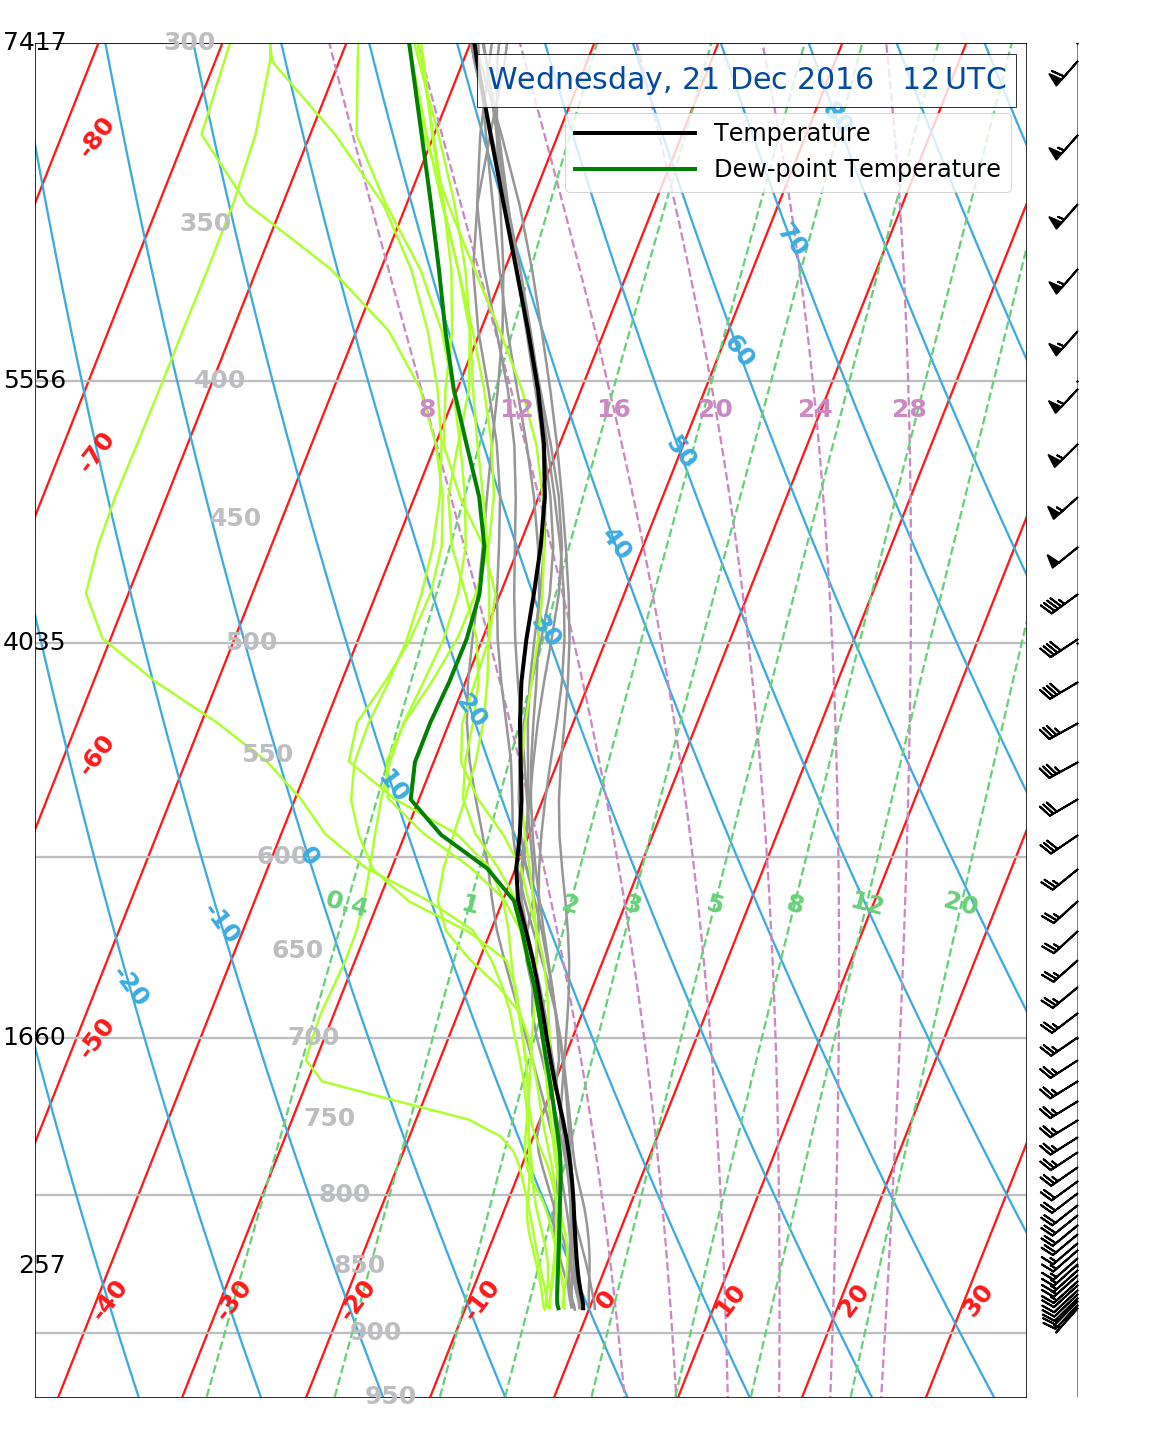
\includegraphics[width=\textwidth]{./fig_Sounding/20161220_36}
		\caption{}\label{fig:meps_sound_20}
	\end{subfigure}
	\begin{subfigure}[b]{0.49\textwidth}
		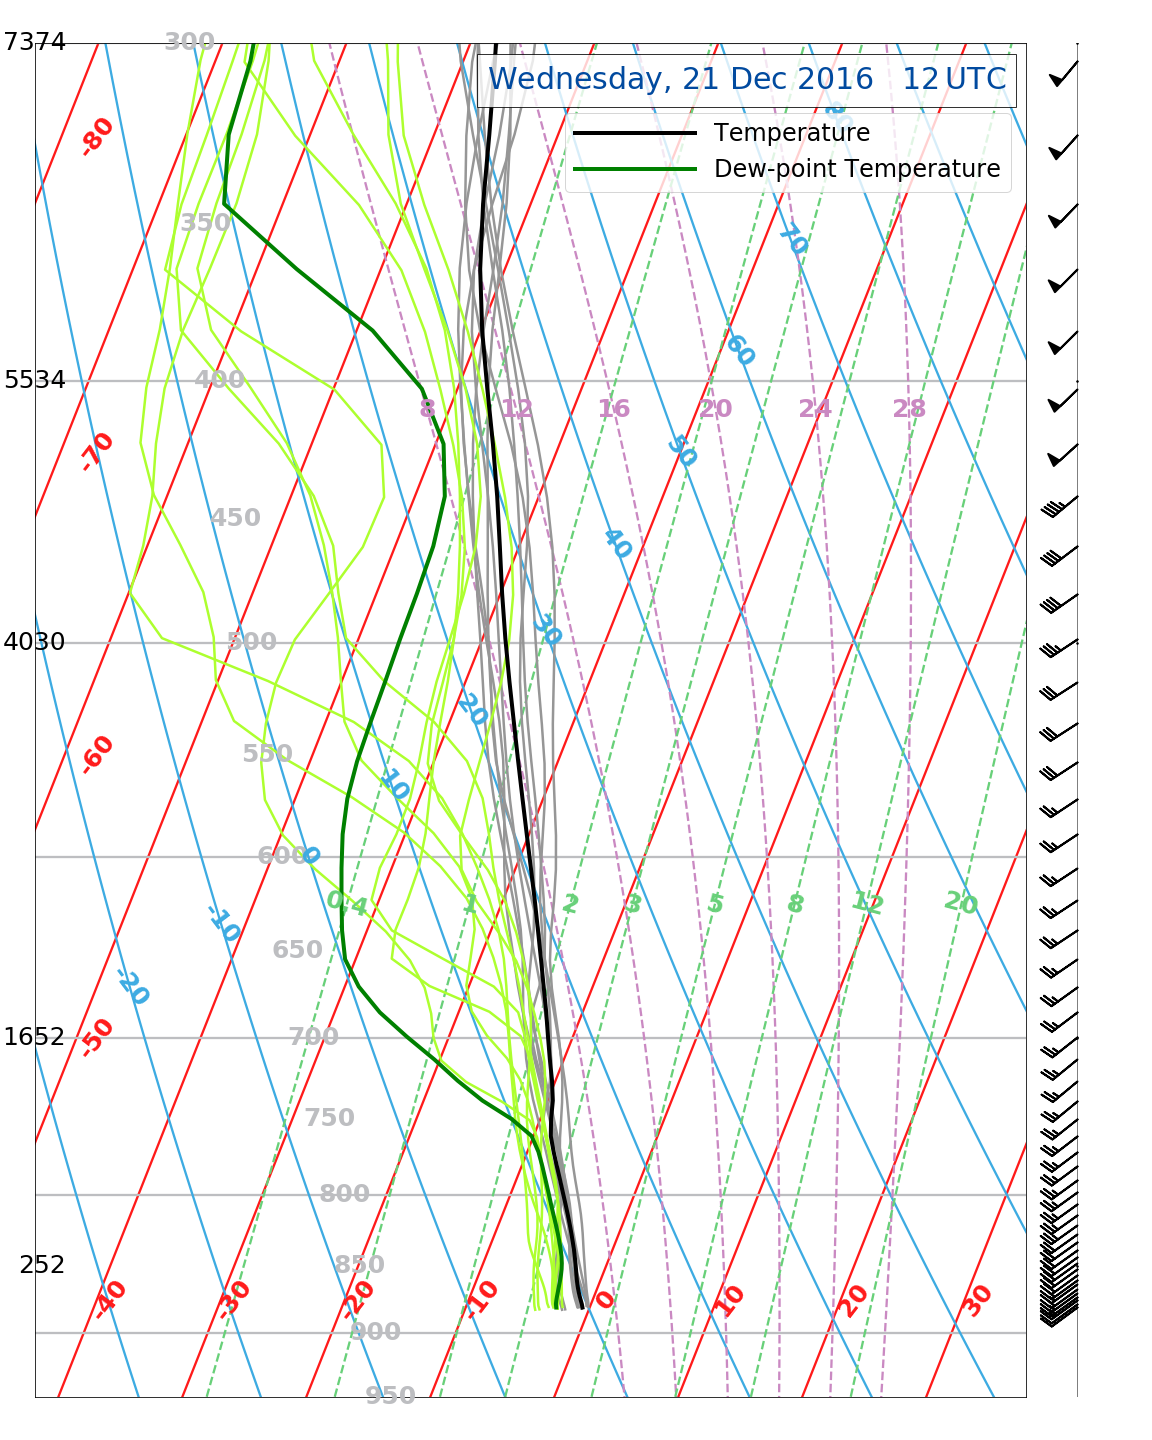
\includegraphics[width=\textwidth]{./fig_Sounding/20161221_12}
		\caption{}\label{fig:meps_sound_21}
	\end{subfigure}
	\caption{Vertical temperature profiles produced with MEPS. \protect{\subref{fig:meps_sound_20}} is initialised: Tuesday, \SI{20}{\dec} \SI{00}{\UTC}. \protect{\subref{fig:meps_sound_21}} is initialised: Wednesday, \SI{21}{\dec} \SI{00}{\UTC}.}
\end{figure}
%%%%%%%%%%%%%%%%%%%%%%%%%%%%%%%%%%%%%%%%%%%%%%%%%%%%%%%%%%%%%%%%%%%%%%%%%%
\textcolor{red}{DISCUSSION! Bring all into relation with the coefficient of variation.}



%%%%%%%%%%%%%%%%%%%%%%%%%%%%%%%%%%%%%%%%%%%%%%%%%%%%%%%%%%%%%%%%%%%%%%%%
\subsection{Saturday, \SI{24}{\dec}}
%%%%%%%%% vertical obs %%%%%%%%%%%%%%
%\subsection{Vertical snowfall observations}
\label{sec:vertEM09:2412}
% %%% image SWP %%%%%%%%%%%%%%%%%%%%%%%%%%%%%%%%%%%%%
\begin{figure}[t]
	\centering
	\begin{subfigure}[t]{\textwidth}
		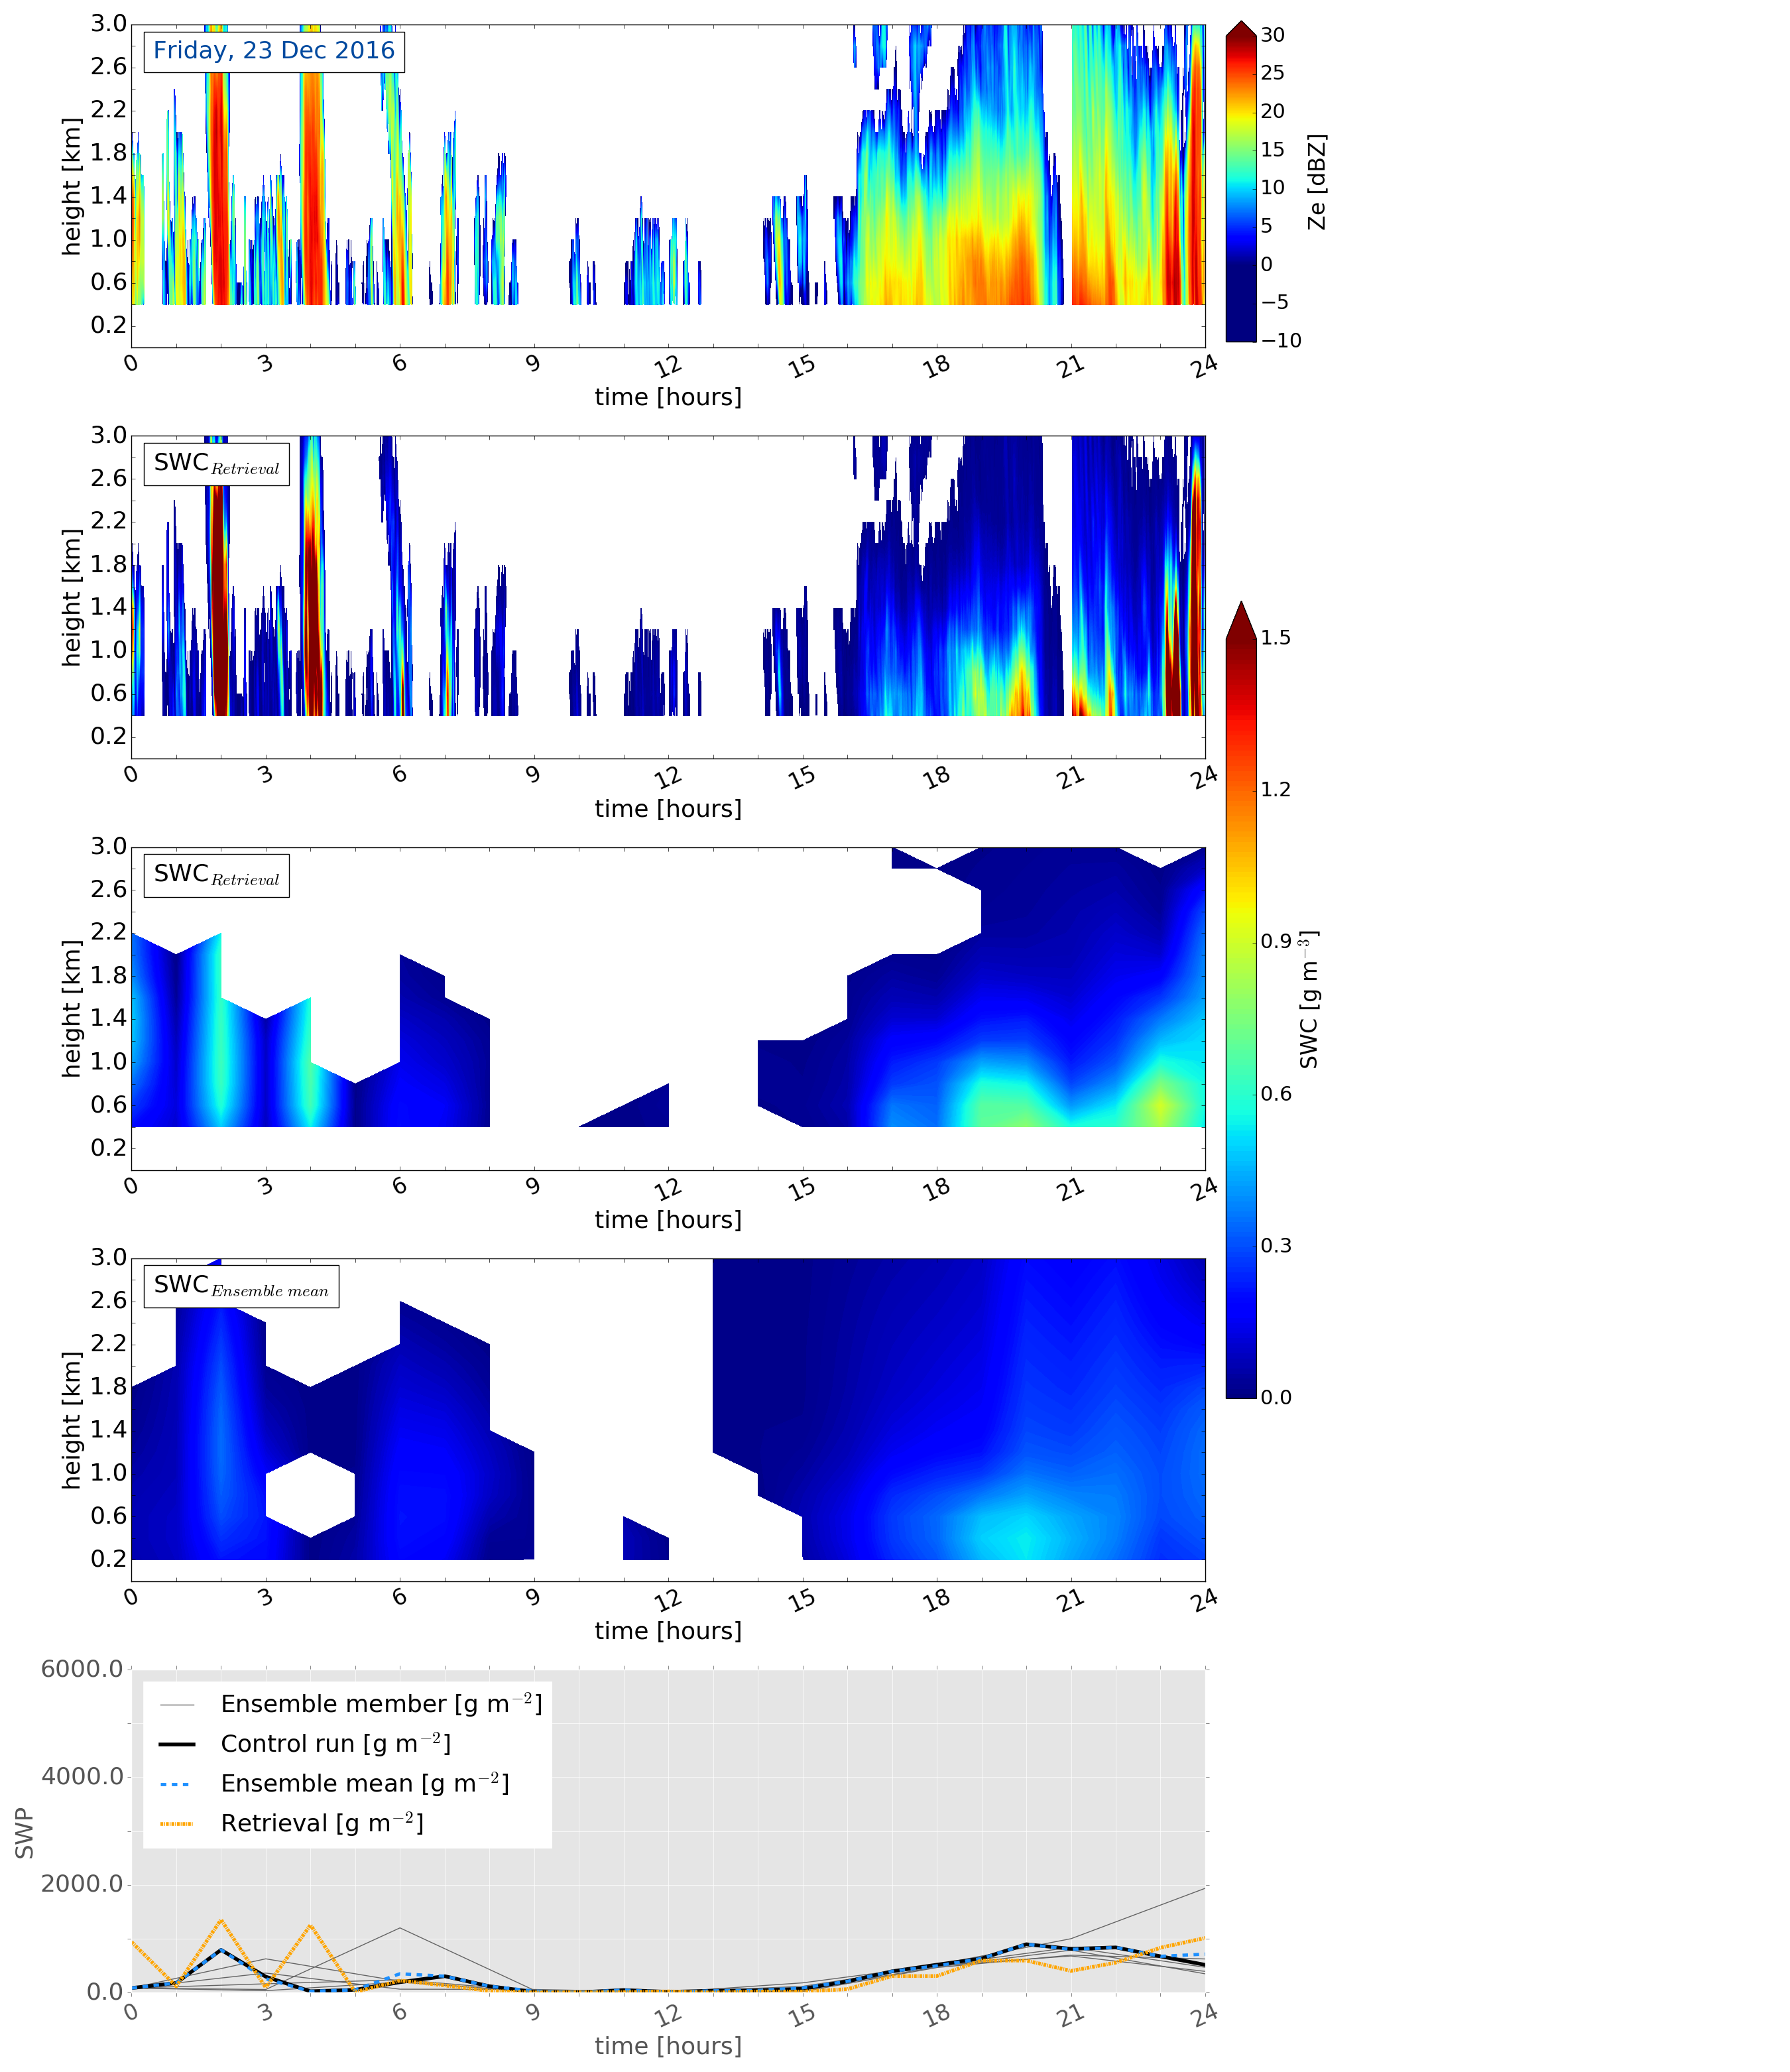
\includegraphics[trim={0.4cm .4cm 31.3cm 63.5cm},clip,width=\textwidth]{./fig_SWC/20161223}
		\caption{}\label{fig:SWP23}
	\end{subfigure}
	\begin{subfigure}[t]{\textwidth}
		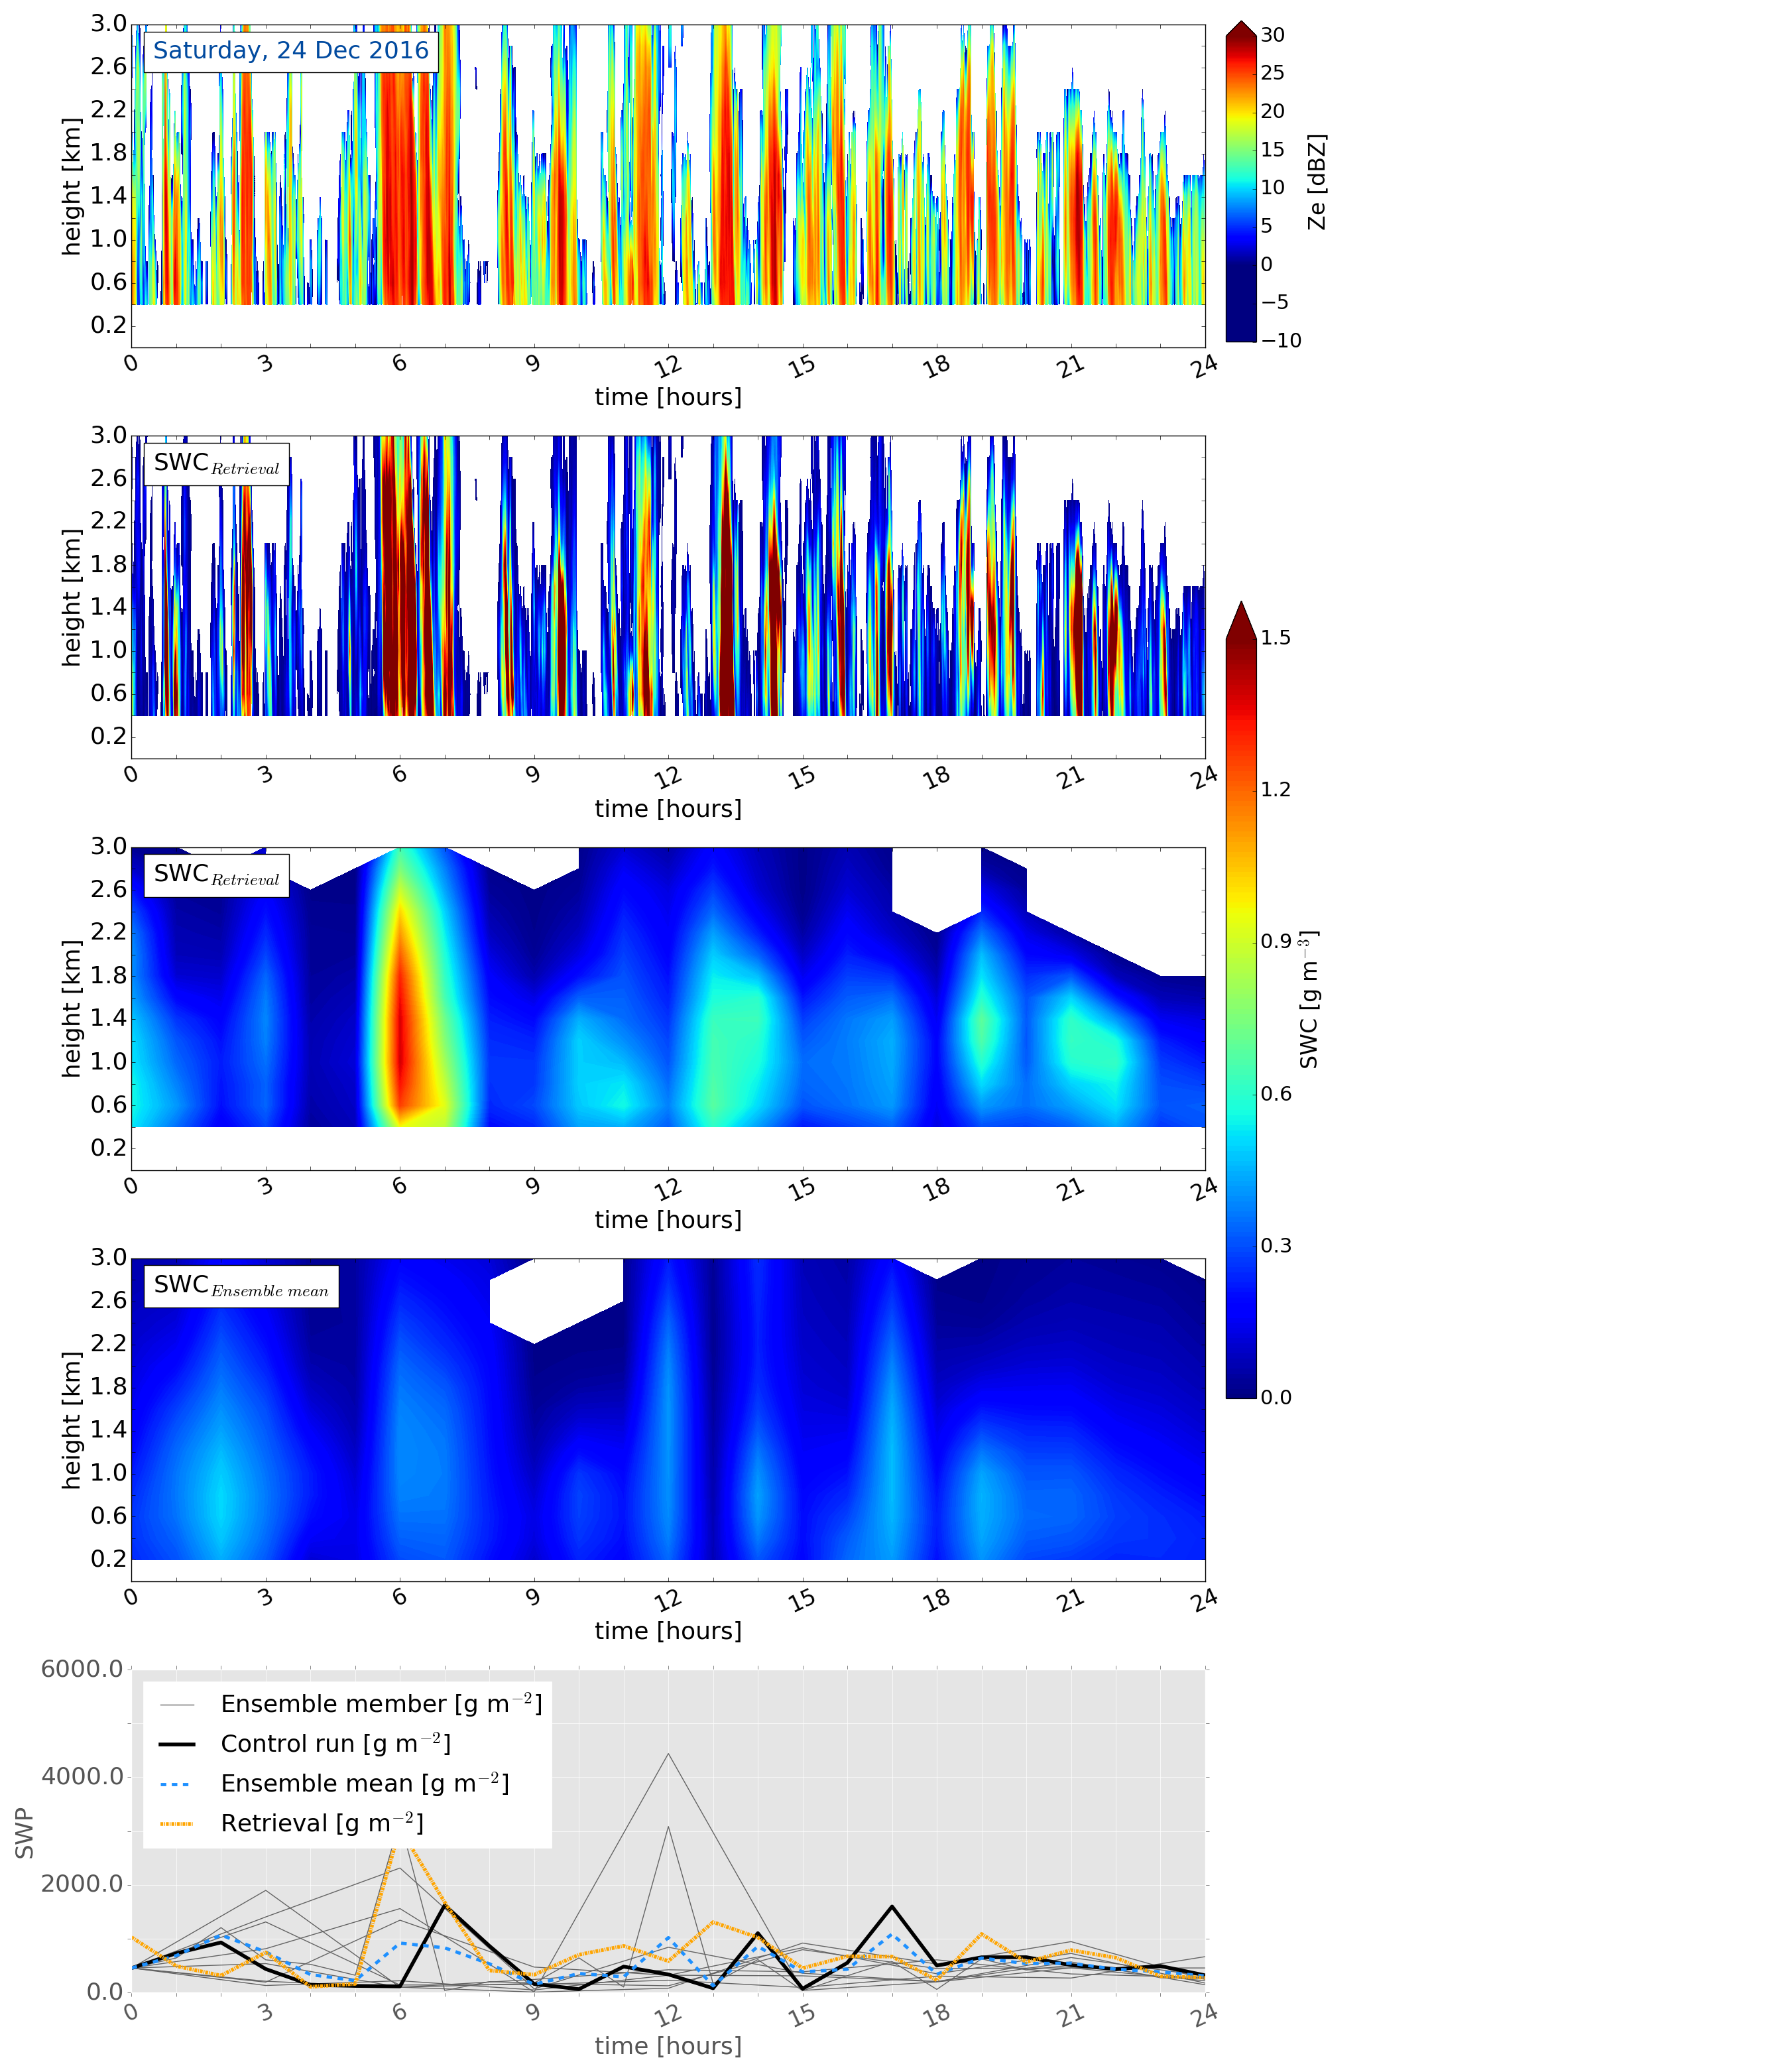
\includegraphics[trim={0.4cm .4cm 31.3cm 63.5cm},clip,width=\textwidth]{./fig_SWC/20161224}
		\caption{}\label{fig:SWP24}
	\end{subfigure}
	\caption{}\label{fig:SWP2324}
\end{figure}
%%%%%%%%%%%%%%%%%%%%%%%%%%%%%%%%%%%%%%%%%%%%%%%%%%%%%%%%%%%%%%%%%%%%%%%%%%
% text
%
% %%% image ensemble member 0-9 %%%%%%%%%%%%%%%%%%%%%%%%%%%%%%%%%%%%%
\begin{figure}[t]
	\centering
	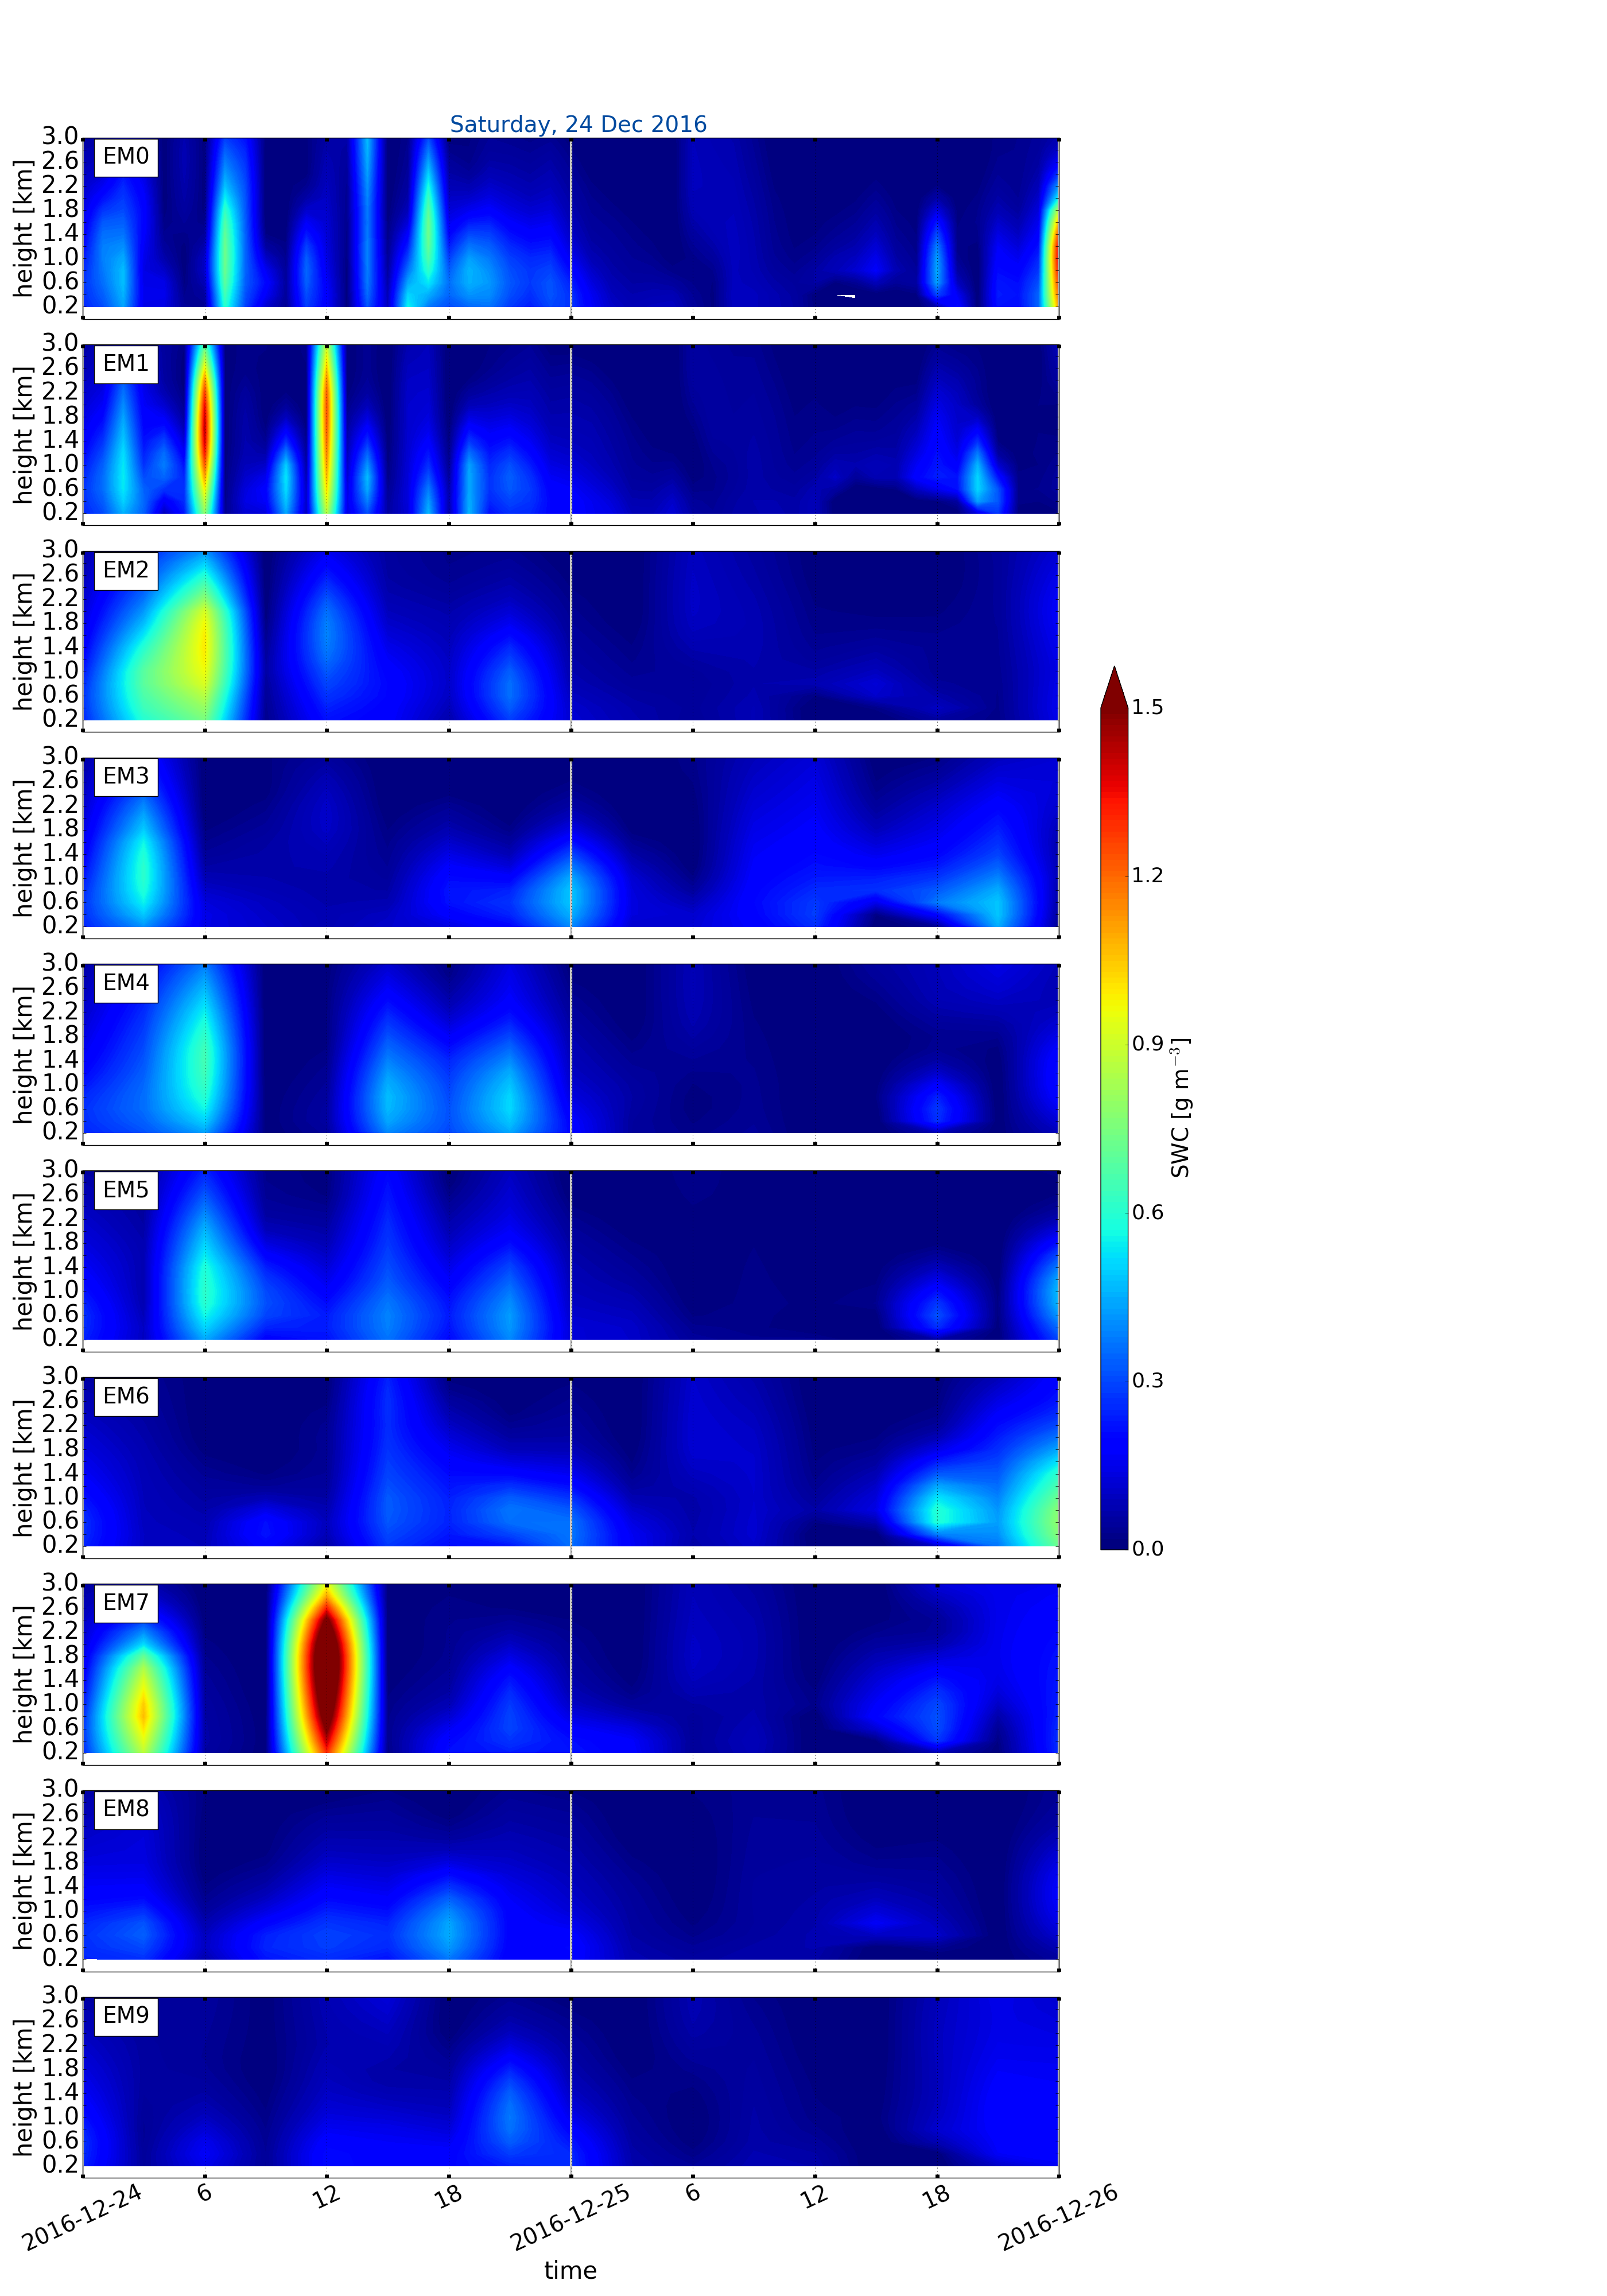
\includegraphics[trim={0cm 0cm 18.3cm 5.1cm},clip,width=0.8\textwidth]{./fig_09EM/20161224}
	\caption{SWC of all ensemble members initialised Saturday, \SI{24}{\dec} at 0\SI{0}{\UTC} forecast for \SI{48}{\hour}.}\label{fig:EM09_24}
\end{figure}
%%%%%%%%%%%%%%%%%%%%%%%%%%%%%%%%%%%%%%%%%%%%%%%%%%%%%%%%%%%%%%%%%%%%%%%%%%
\textcolor{red}{DISCUSSION! Bring all into relation and include the verification plots}
\begin{itemize}
	\item Because EM3, EM4, EM7 to EM9 are only valid every three hours can precipitation peaks not crop up in such a high frequency as for example the deterministic forecast. 
\end{itemize}


%%%%%%%%%%%%%%%%%%%%%%%%%%%%%%%%%%%%%%%%%%%%%%%%%%%%%%%%%%%%%%%%%%%%%%%%
\subsection{Sunday, \SI{25}{\dec}}
%%%%%%%%% vertical obs %%%%%%%%%%%%%%
%\subsection{Vertical snowfall observations}
\label{sec:vertEM09:2512}
% %%% image SWP %%%%%%%%%%%%%%%%%%%%%%%%%%%%%%%%%%%%%
\begin{figure}[t]
	\centering
	\begin{subfigure}[t]{\textwidth}
		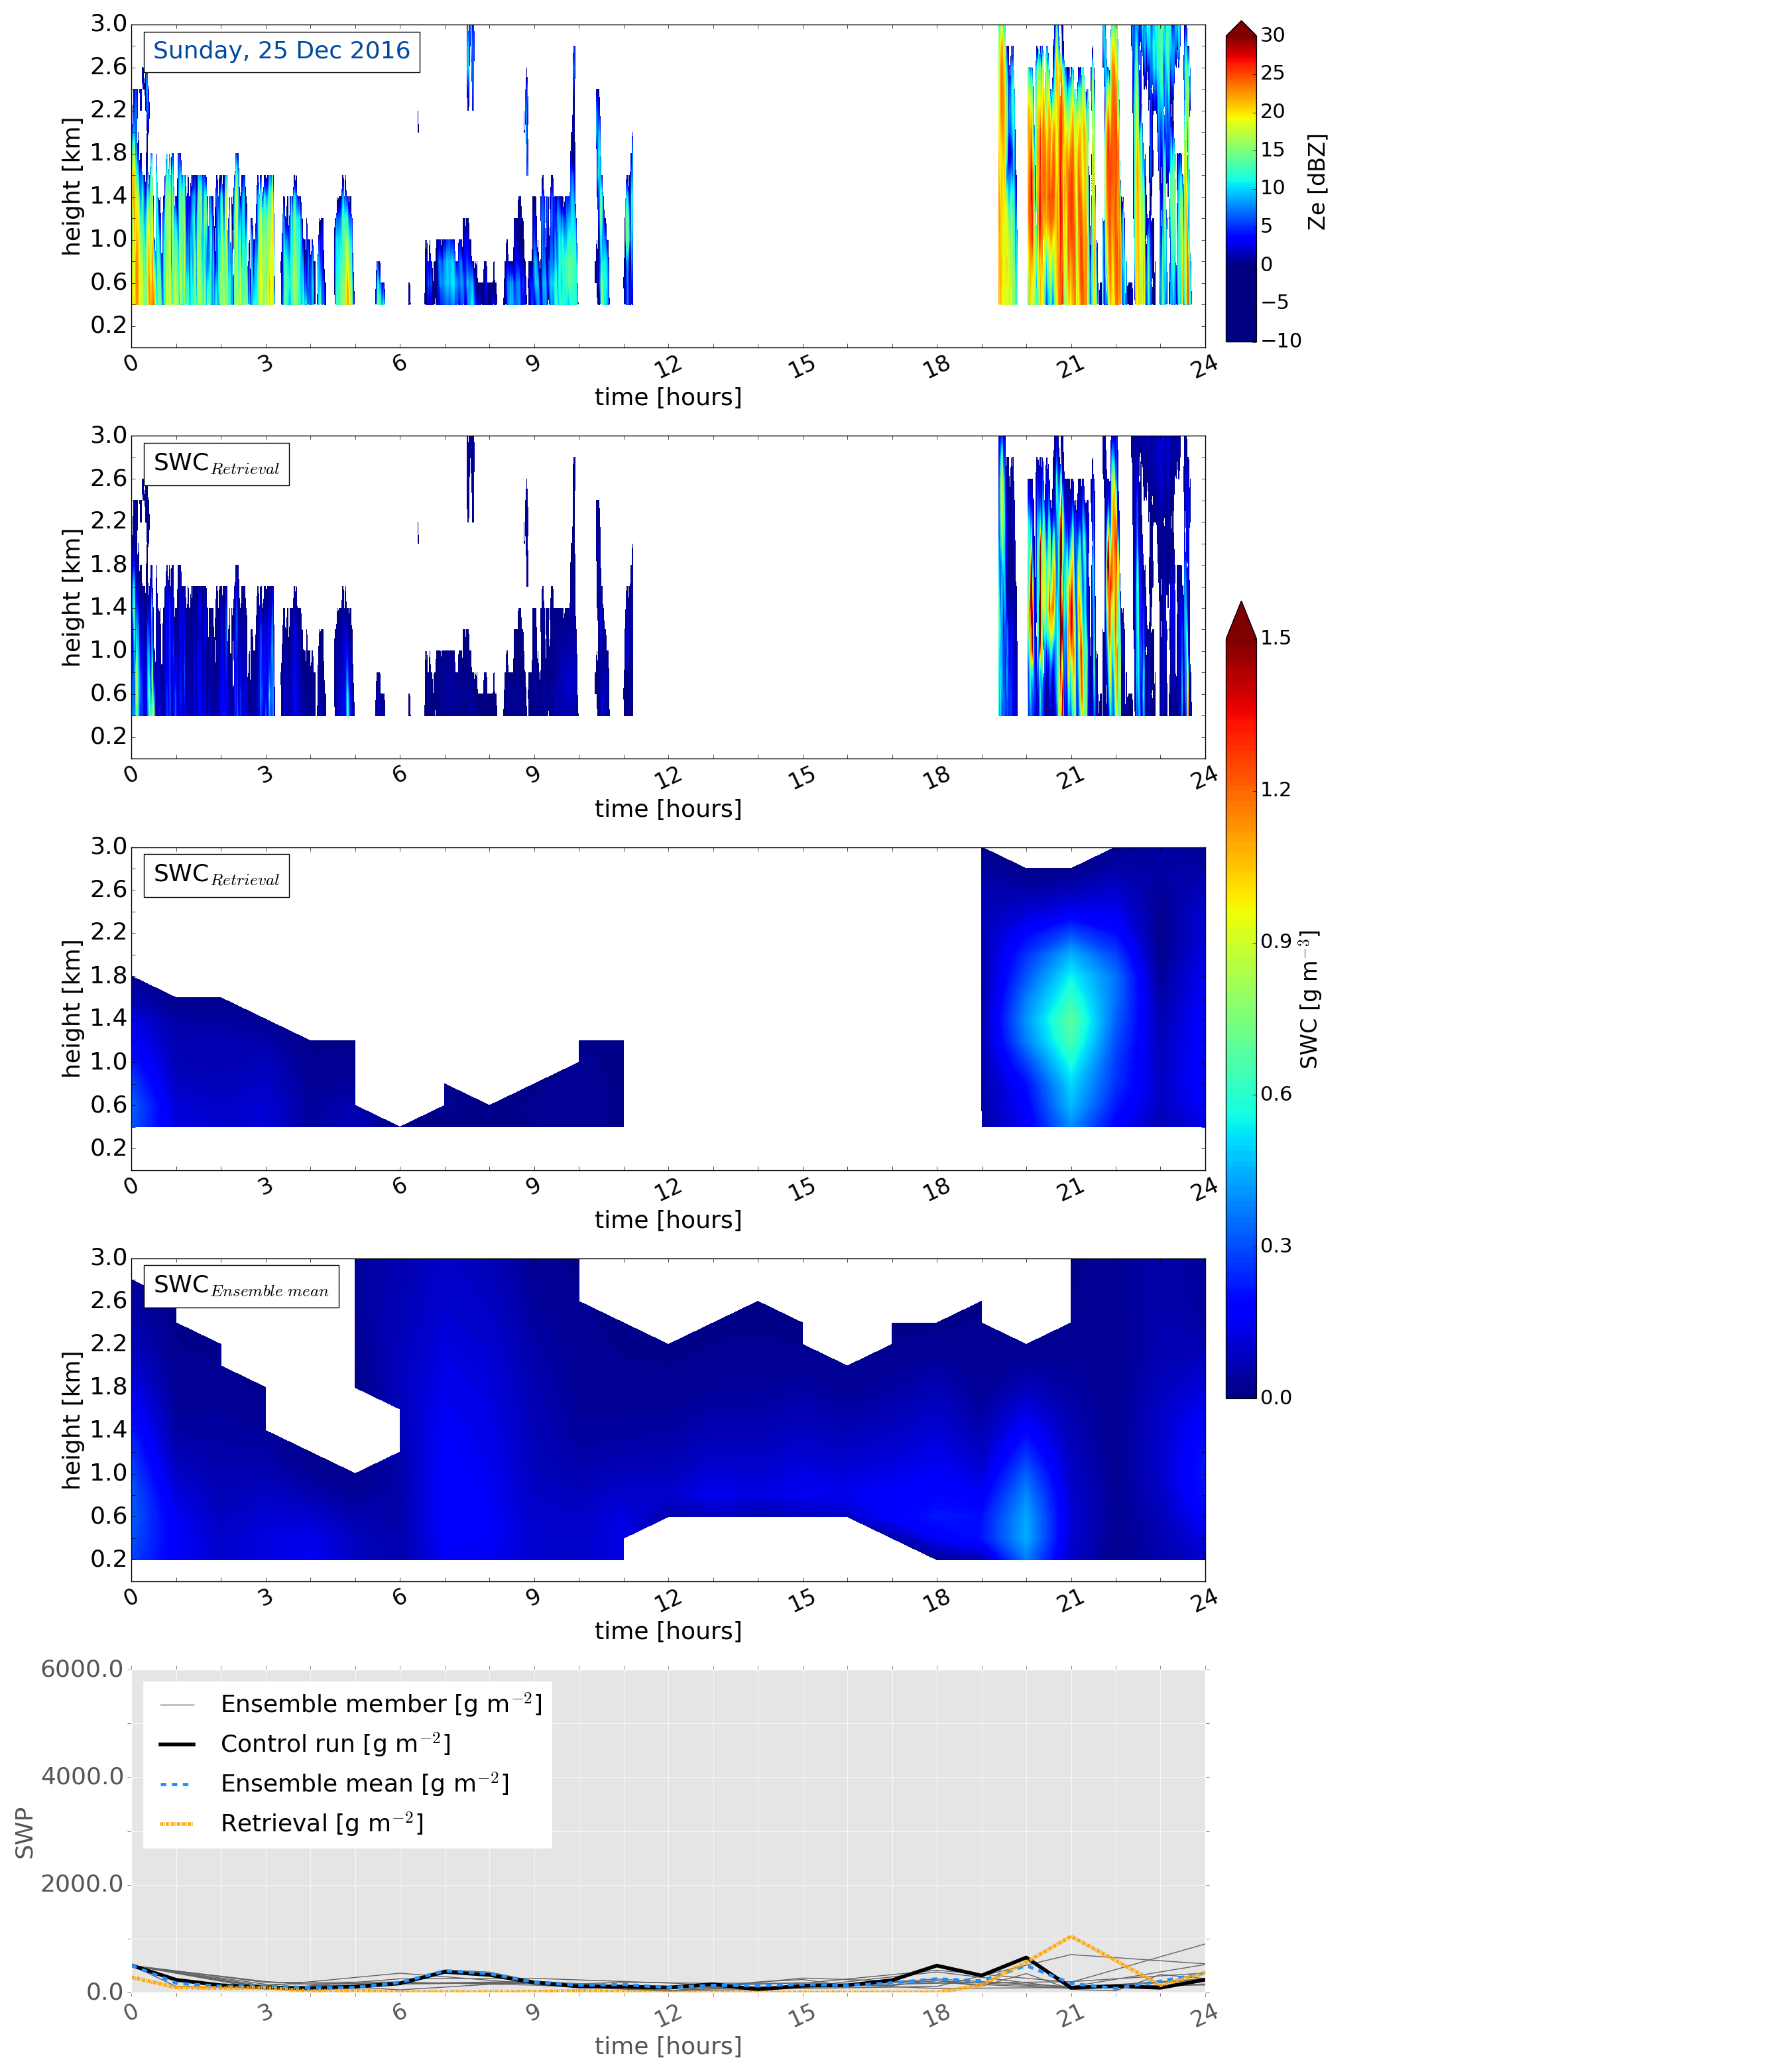
\includegraphics[trim={0.4cm .4cm 31.3cm 63.5cm},clip,width=\textwidth]{./fig_SWC/20161225}
	\end{subfigure}
	\caption{}\label{fig:SWP25}
\end{figure}
%%%%%%%%%%%%%%%%%%%%%%%%%%%%%%%%%%%%%%%%%%%%%%%%%%%%%%%%%%%%%%%%%%%%%%%%%%
% text
%
% %%% image ensemble member 0-9 %%%%%%%%%%%%%%%%%%%%%%%%%%%%%%%%%%%%%
\begin{figure}[t]
	\centering
	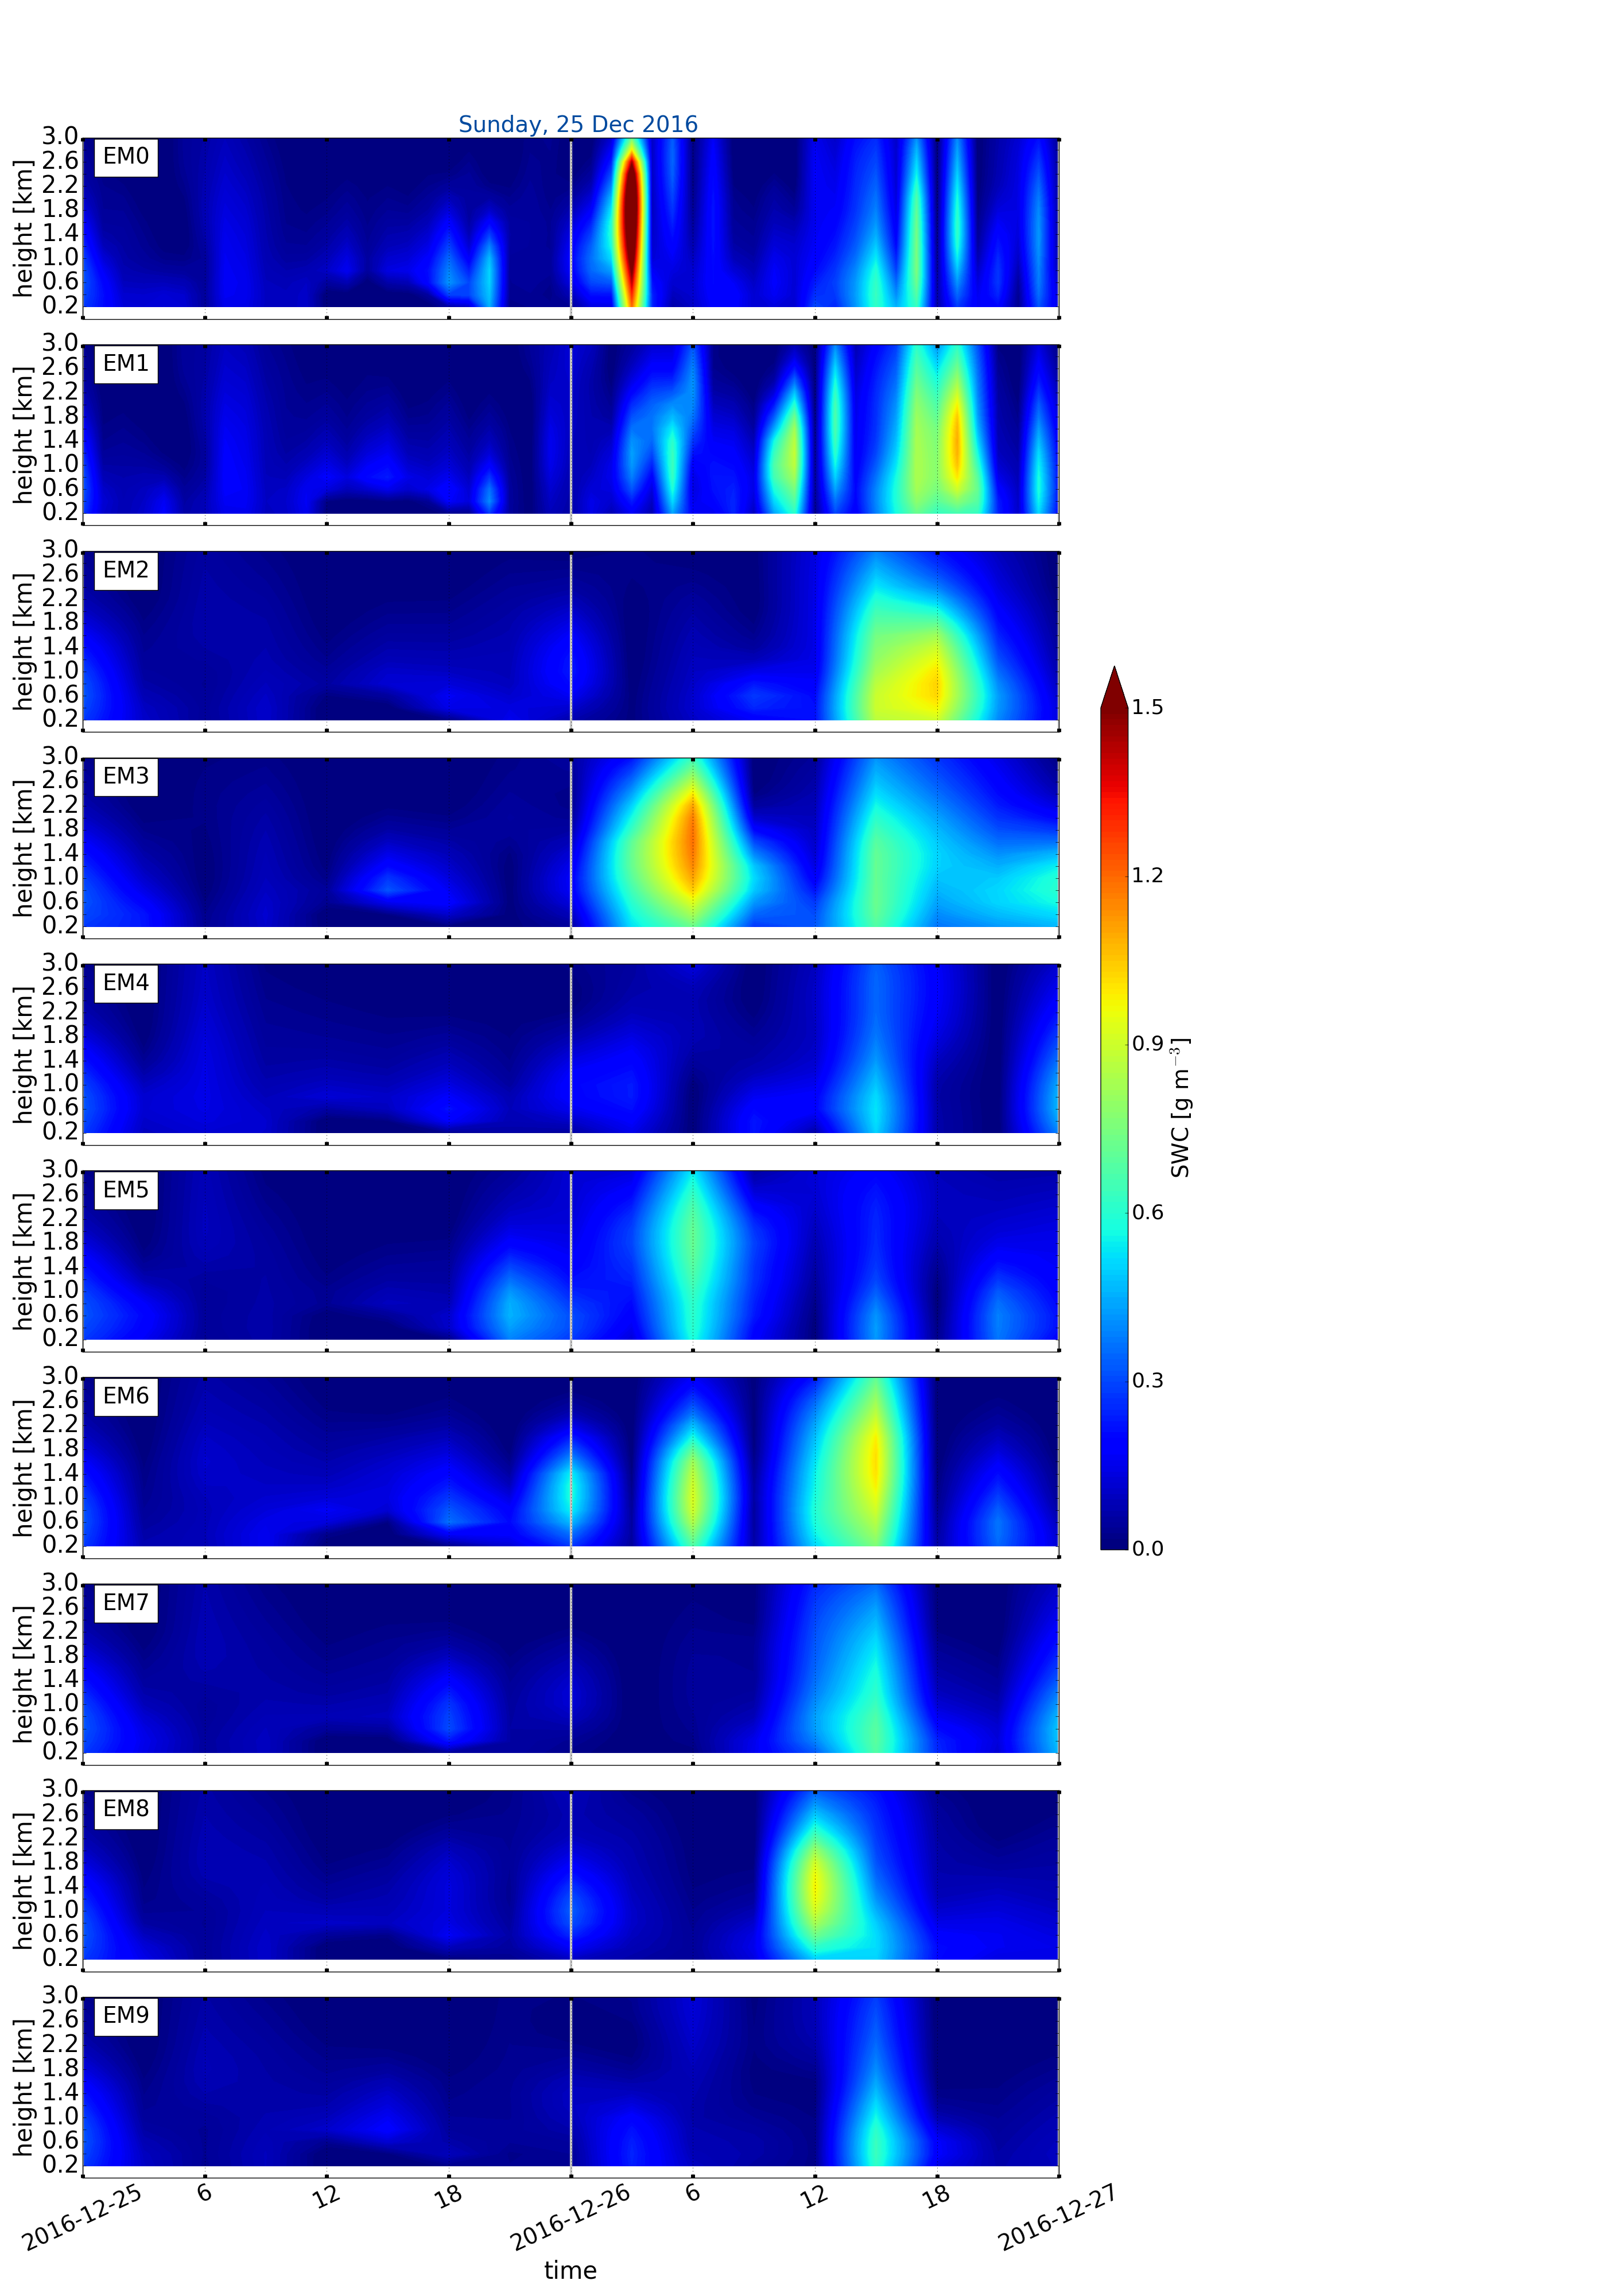
\includegraphics[trim={0cm 0cm 18.3cm 5.1cm},clip,width=0.8\textwidth]{./fig_09EM/20161225}
	\caption{SWC of all ensemble members initialised Sunday, \SI{25}{\dec} at 0\SI{0}{\UTC} forecast for \SI{48}{\hour}.}\label{fig:EM09_25}
\end{figure}
%%%%%%%%%%%%%%%%%%%%%%%%%%%%%%%%%%%%%%%%%%%%%%%%%%%%%%%%%%%%%%%%%%%%%%%%%%
\textcolor{red}{DISCUSSION! Bring all into relation and include the verification plots}
%%%%%%%%%%%%%%%%%%%%%%%%%%%%%%%%%%%%%%%%%%%%%%%%%%%%%%%%%%%%%%%%%%%%%%%%




%%%%%%%%%%%%%%%%%%%%%%%%%%%%%%%%%%%%%%%%%%%%%%%%%%%%%%%%%%%%%%%%%%%%%%%%%
%%%%%%%% 21122016 24122016 25122016 %%%%%%%%%%%%%%
% !TeX spellcheck = en_GB
\section{Wednesday, \SI{21}{\dec}}

Convection appears: see \Cref{fig:meps_sound_20} and \ref{fig:meps_sound_21}, also \Cref{fig:Soun21}
%
%%% image sounding MEPS %%%%%%%%%%%%%%%%%%%%%%%%%%%%%%%%%%%%%
% !TeX spellcheck = en_GB
\begin{figure}
	\centering
	\begin{subfigure}[b]{0.49\textwidth}
		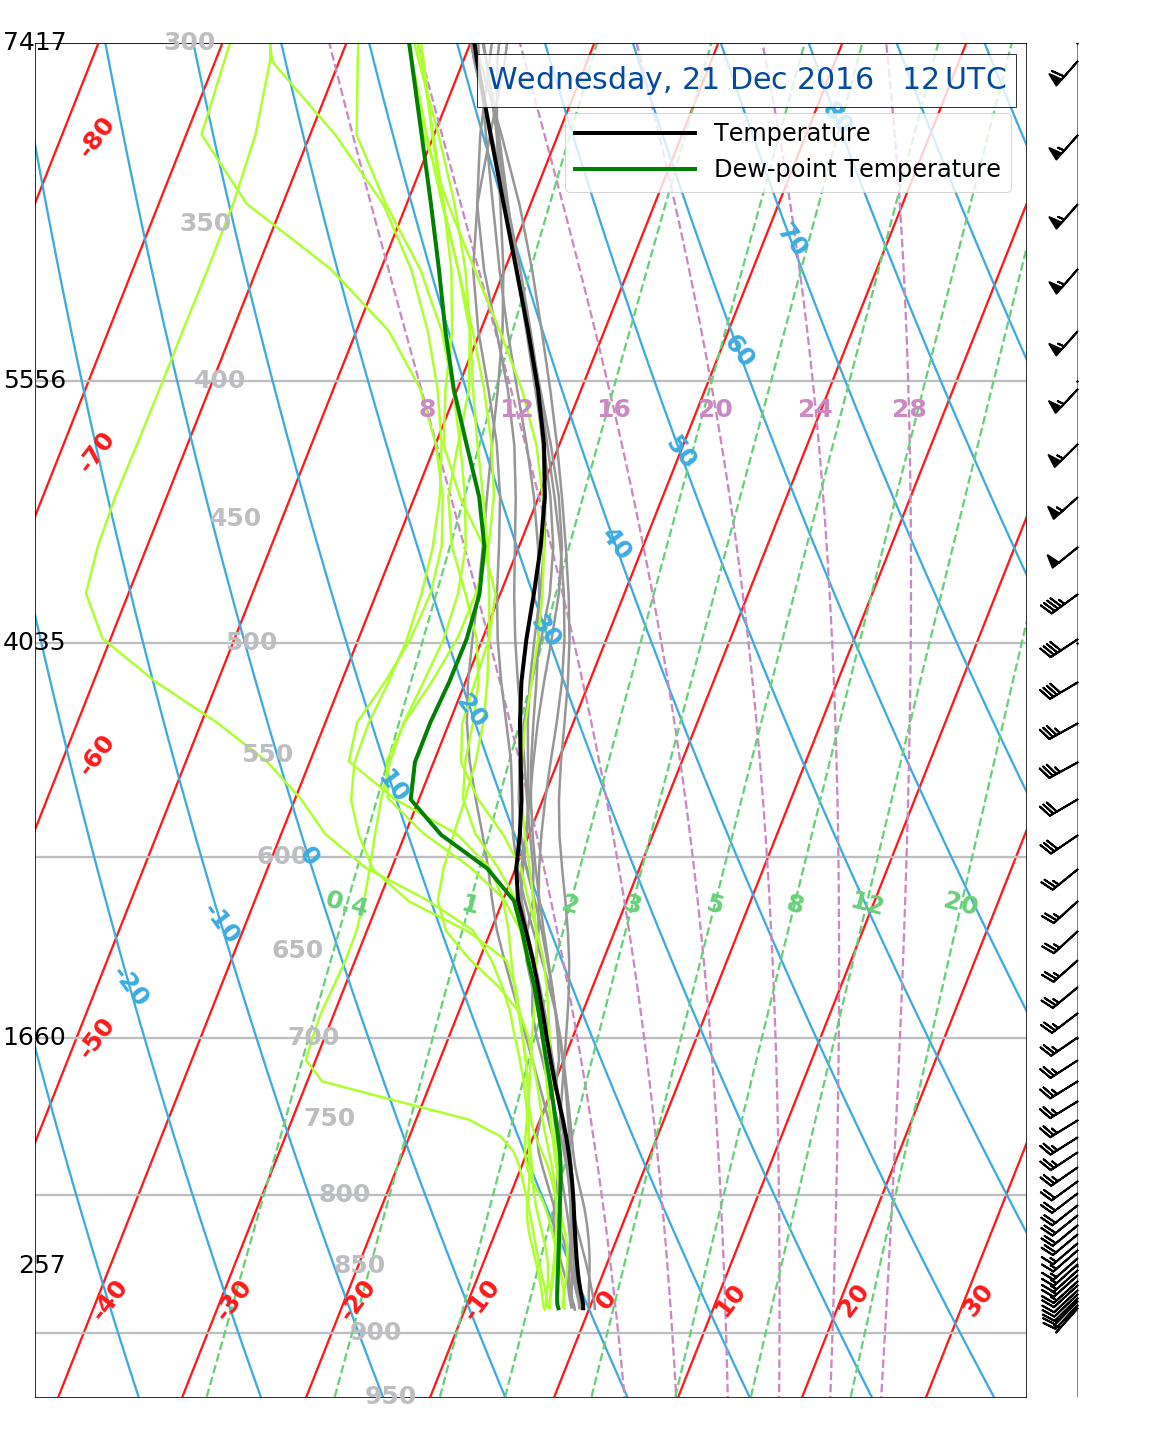
\includegraphics[width=\textwidth]{./fig_Sounding/20161220_36}
		\caption{}\label{fig:meps_sound_20}
	\end{subfigure}
	\begin{subfigure}[b]{0.49\textwidth}
		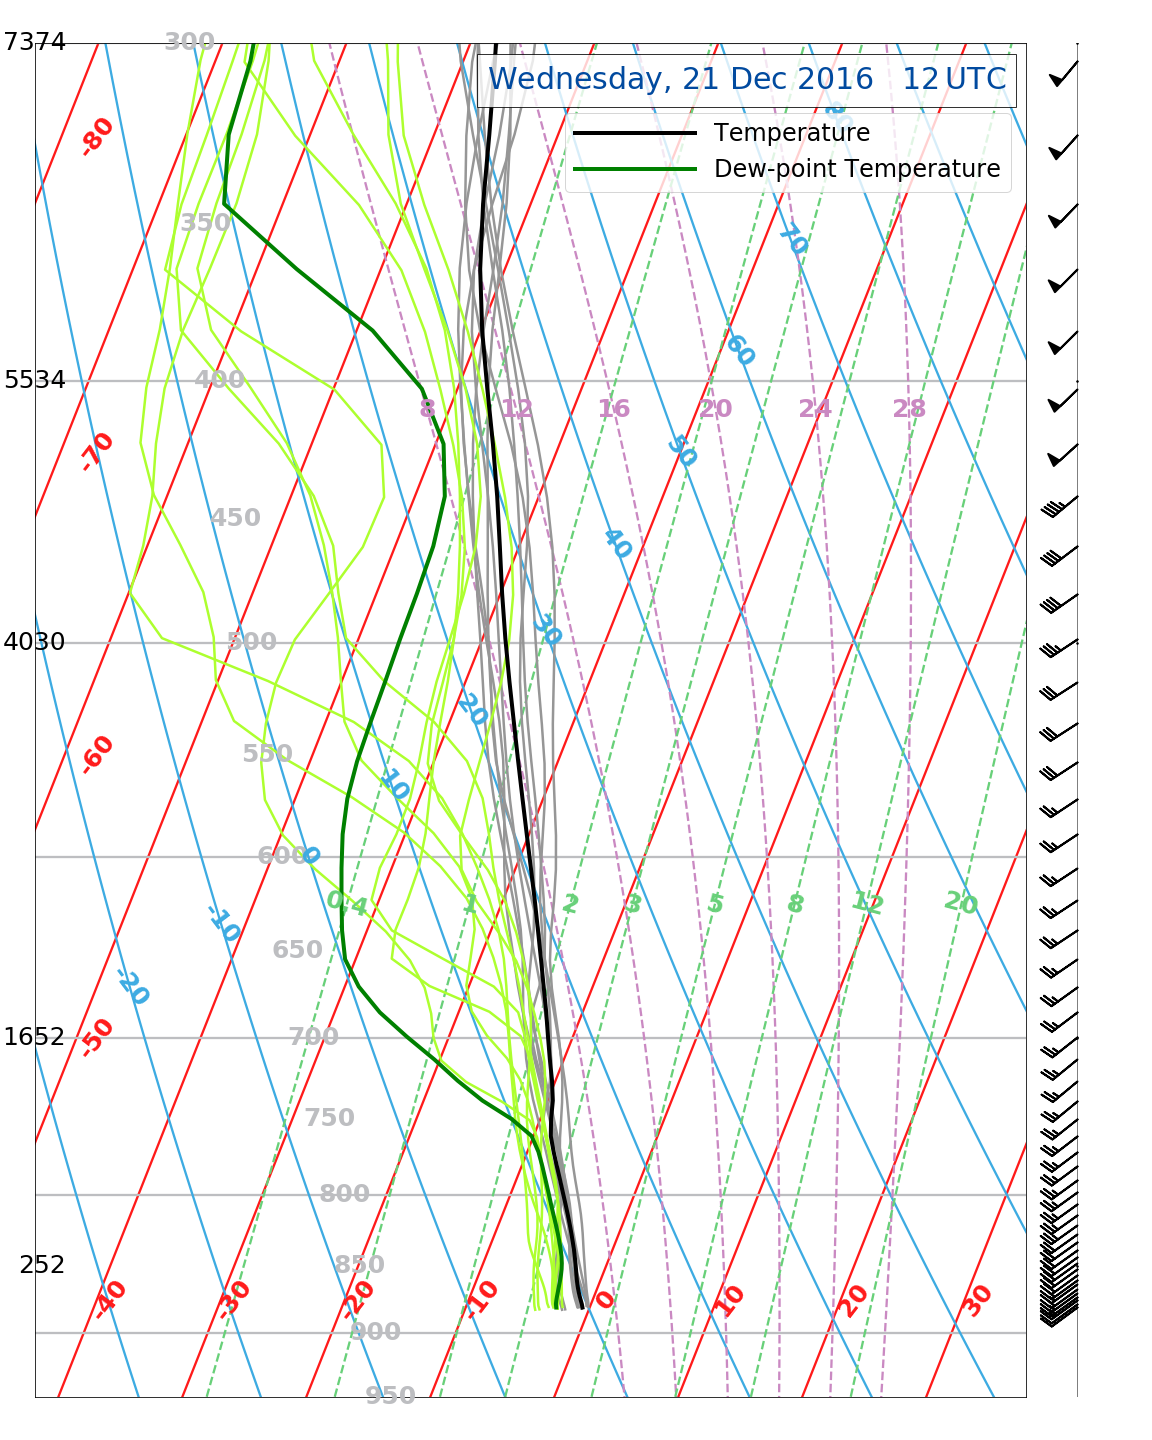
\includegraphics[width=\textwidth]{./fig_Sounding/20161221_12}
		\caption{}\label{fig:meps_sound_21}
	\end{subfigure}
	\caption{Vertical temperature profiles produced with MEPS. \protect{\subref{fig:meps_sound_20}} is initialised: Tuesday, \SI{20}{\dec} \SI{00}{\UTC}. \protect{\subref{fig:meps_sound_21}} is initialised: Wednesday, \SI{21}{\dec} \SI{00}{\UTC}.}
\end{figure}
%%%%%%%%%%%%%%%%%%%%%%%%%%%%%%%%%%%%%%%%%%%%%%%%%%%%%%%%%%%%%%%%%%%%%%%%%%


%%%%%%%%%%%%%%%%%%%%%%%%%%%%%%%%%%%%%%%%%%%%%%%%%%%%%%%%%%%%%%%%%%%%%%%%%
%%%%%%%% 24122016 %%%%%%%%%%%%%%
%%%%%%%%%%%%%%%%%%%%%
% !TeX spellcheck = en_GB
\section{Saturday, \SI{24}{\dec}}\label{sec:2412}

%%% short info on Saturdays general weather


%%%%%%%%%%%%%%%%%%%%%%%%%%%%%%%%%%%%%%%%%%%%%%%%%%%%%%%%%%%%%%%%%%%%%%%%%%
%%%%%%%%% surface obs %%%%%%%%%%%%%%
\subsection{Surface accumulation}
% text 

%%% image surface MEPS boxplot %%%%%%%%%%%%%%%%%%%%%%%%%%%%%%%%%%%%%
\begin{figure}[t]
	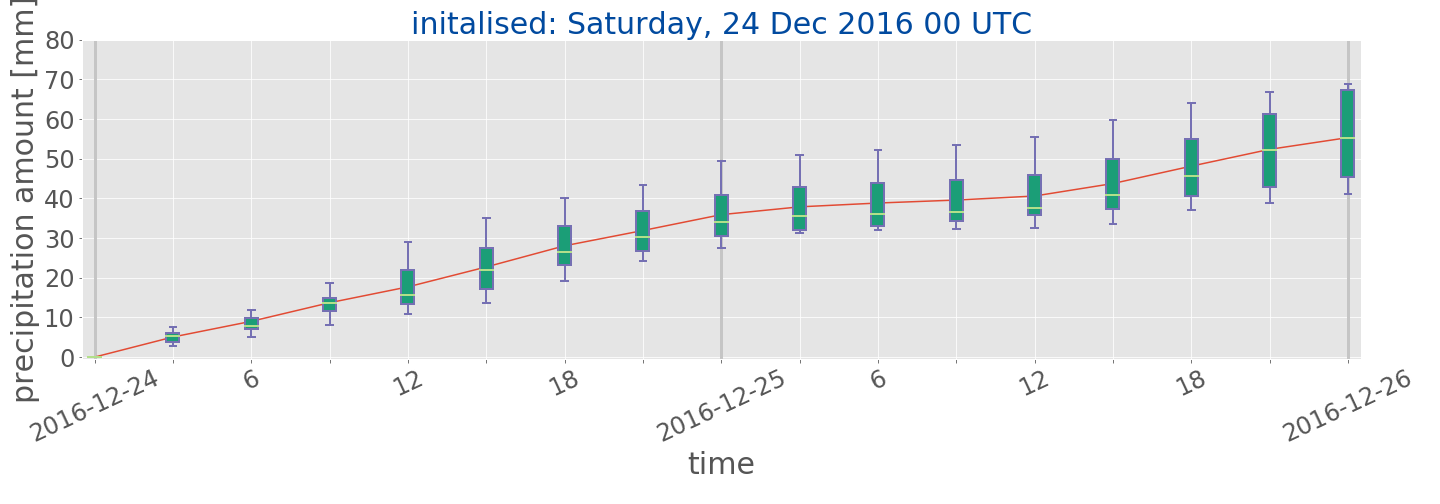
\includegraphics[width=\textwidth]{./fig_boxplot_sfc/20161224_0}
	\caption{Box-whisker-plot of the ten ensemble members of MEPS. Red line indicating the ensemble mean, lower and upper whisker the 25th and 75th percentile, respectively. Light green shows the median of all members and the box represents the middle \SI{50}{\percent} of scores of the precipitation.}\label{fig:boxplt24}
\end{figure}
%%%%%%%%%%%%%%%%%%%%%%%%%%%%%%%%%%%%%%%%%%%%%%%%%%%%%%%%%%%%%%%%%%%%%%%%%%
The box-whisker-plot in \Cref{fig:boxplt24} shows an uncertainty shortly after initialisation of the ten forecast members. All members have a different opinion of the precipitation amount, since the difference between the \SIrange{25}{75}{\percent} is wide spread.
The ensemble mean is always higher than the median and already after \SI{12}{\hour} forecast time is the median closer to the lower percentile. Also, all upper whiskers are taller than the lower ones, which would follow that the ensemble members vary amongst the most positive quartile and that it is very similar for the least positive quartile group.
\\
\textcolor{red}{DISCUSSION! The uncertainty shortly after the initialisation time might be associated with the spin up time of the precipitation value in the model. }
%%%%%%%%%%%%%%%%%%%%%%%%%%%%%%%%%%%%%%%%%%%%%%%%%%%%%%%%%%%%%%%%%%%%%%%%%%
%%%%%%%%% vertical obs %%%%%%%%%%%%%%
\subsection{Vertical snowfall observations}\label{sec:vertEM09:2412}
% %%% image SWP %%%%%%%%%%%%%%%%%%%%%%%%%%%%%%%%%%%%%
\begin{figure}[t]
	\centering
	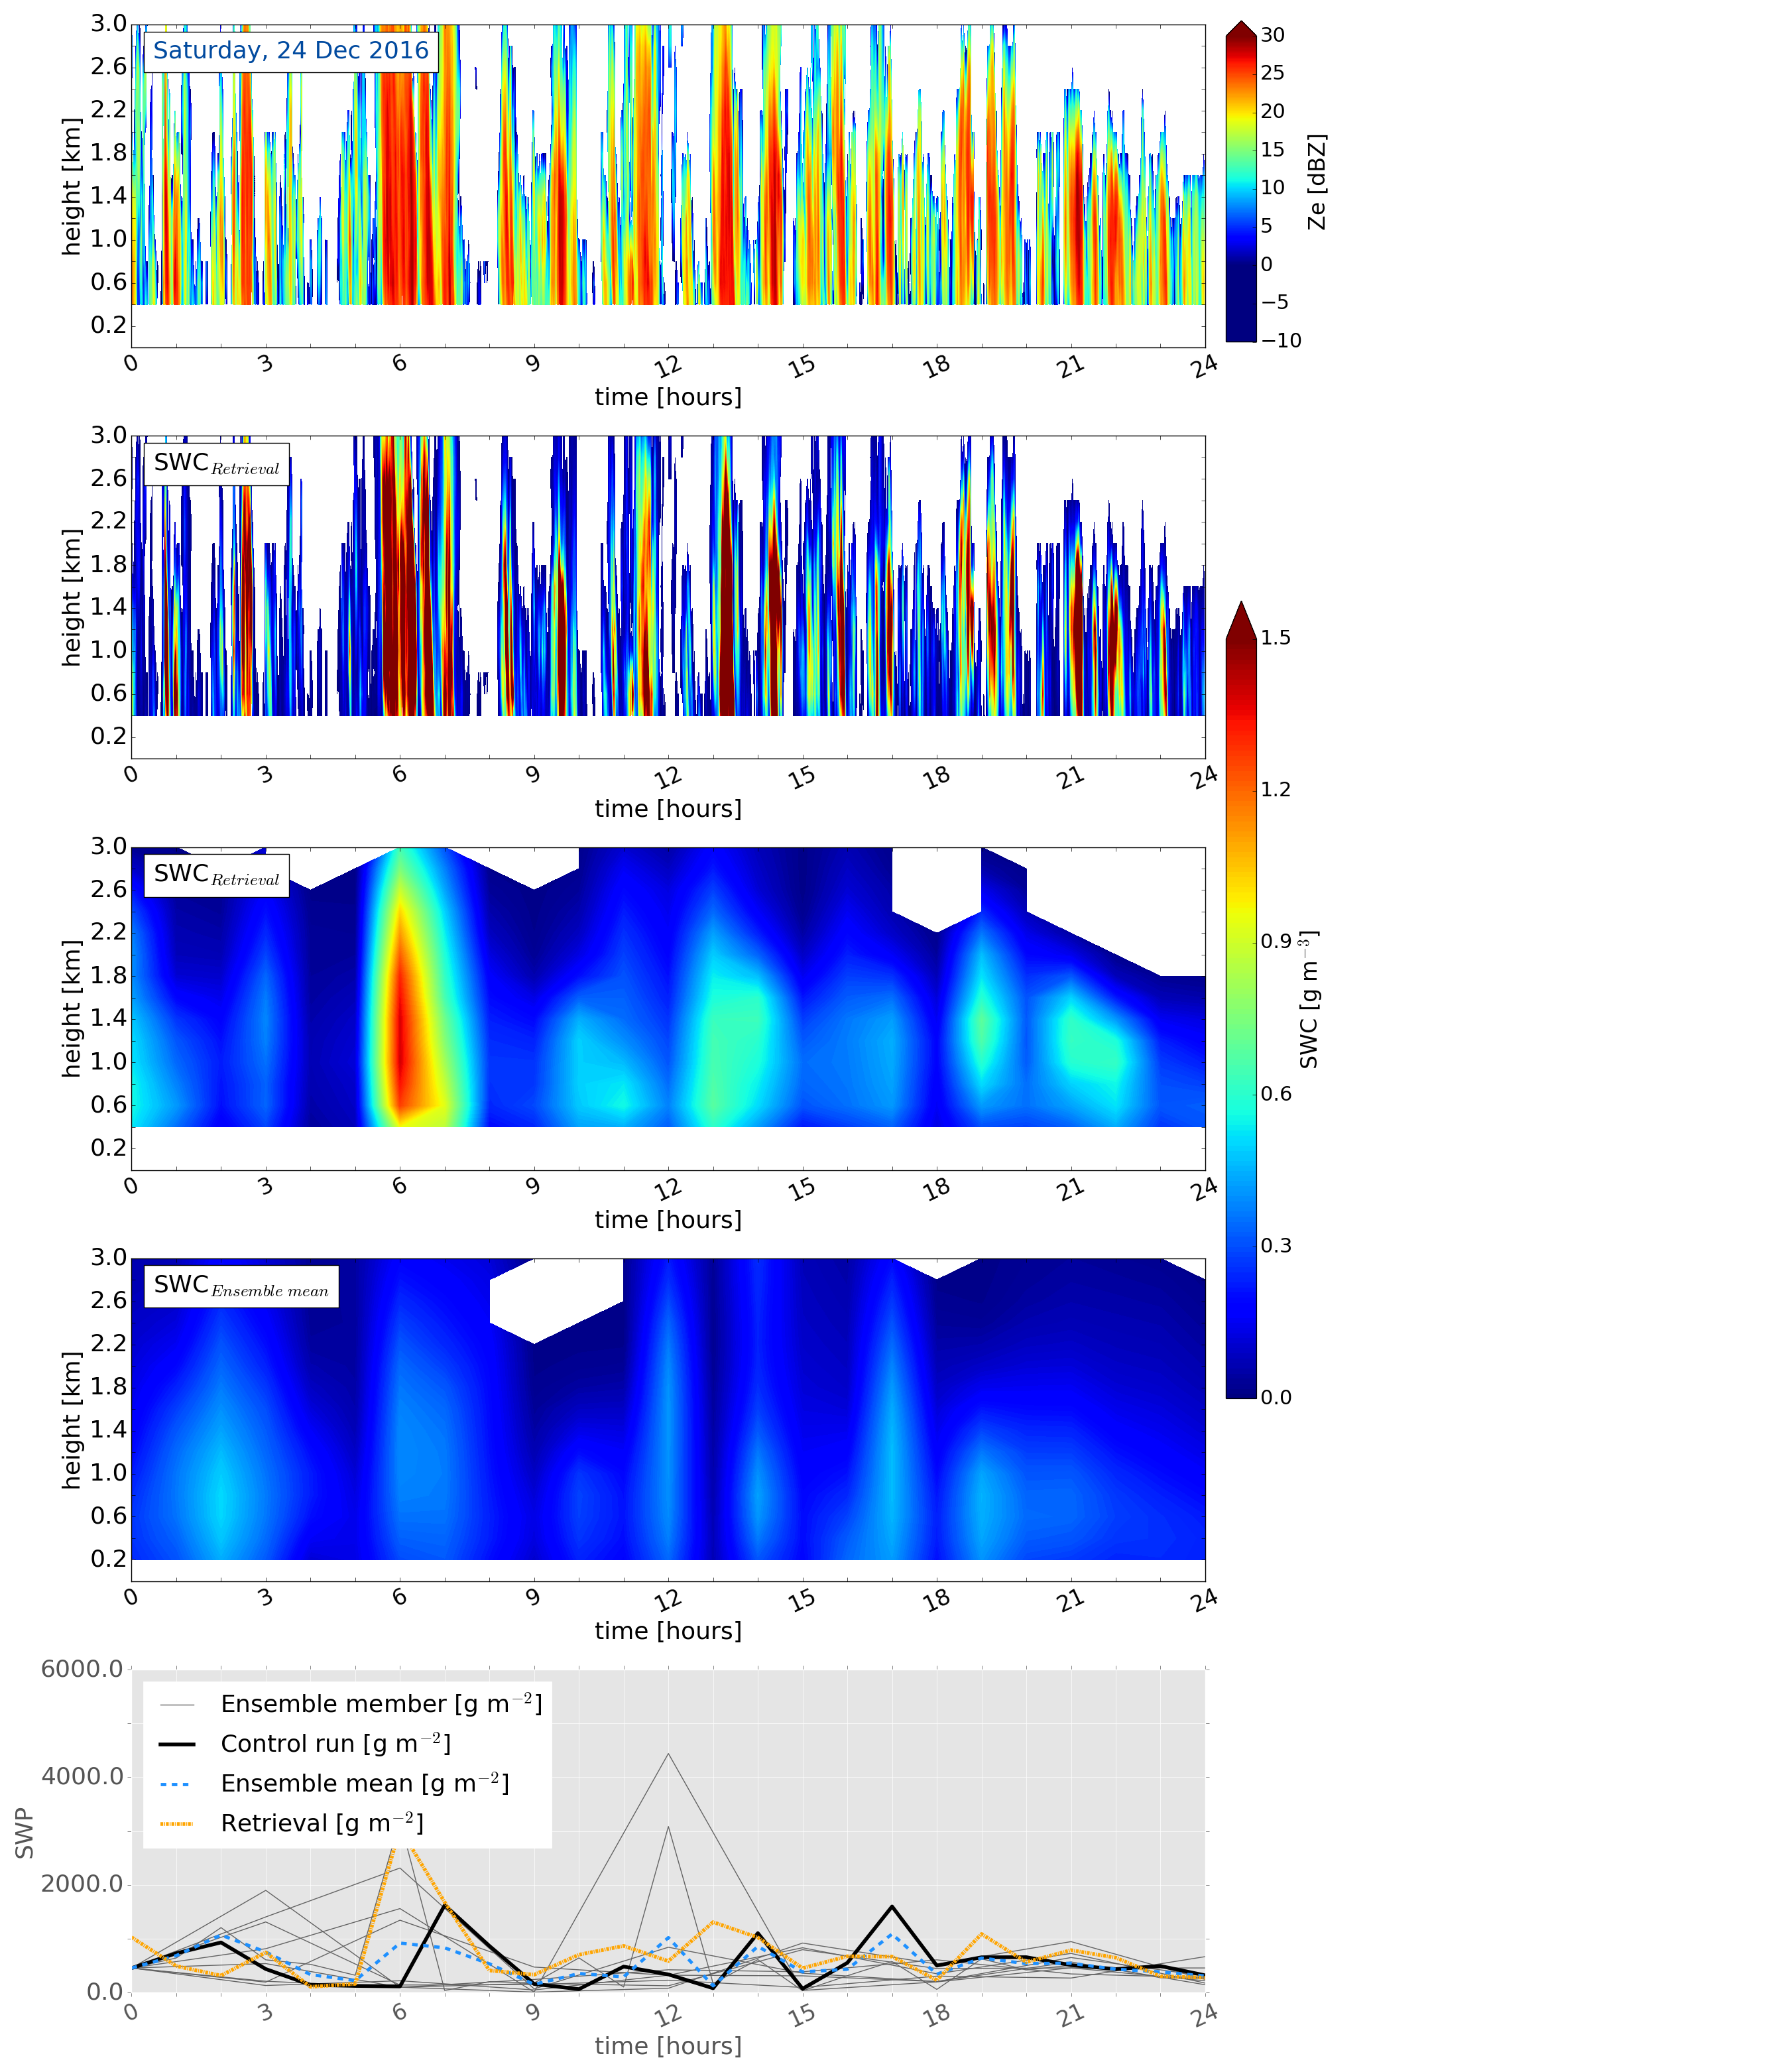
\includegraphics[trim={0.4cm .4cm 31.3cm 63.5cm},clip,width=\textwidth]{./fig_SWC/20161224}
	\caption{}\label{fig:SWP24}
\end{figure}
%%%%%%%%%%%%%%%%%%%%%%%%%%%%%%%%%%%%%%%%%%%%%%%%%%%%%%%%%%%%%%%%%%%%%%%%%%
% text
%
% %%% image ensemble member 0-9 %%%%%%%%%%%%%%%%%%%%%%%%%%%%%%%%%%%%%
\begin{figure}[t]
	\centering
	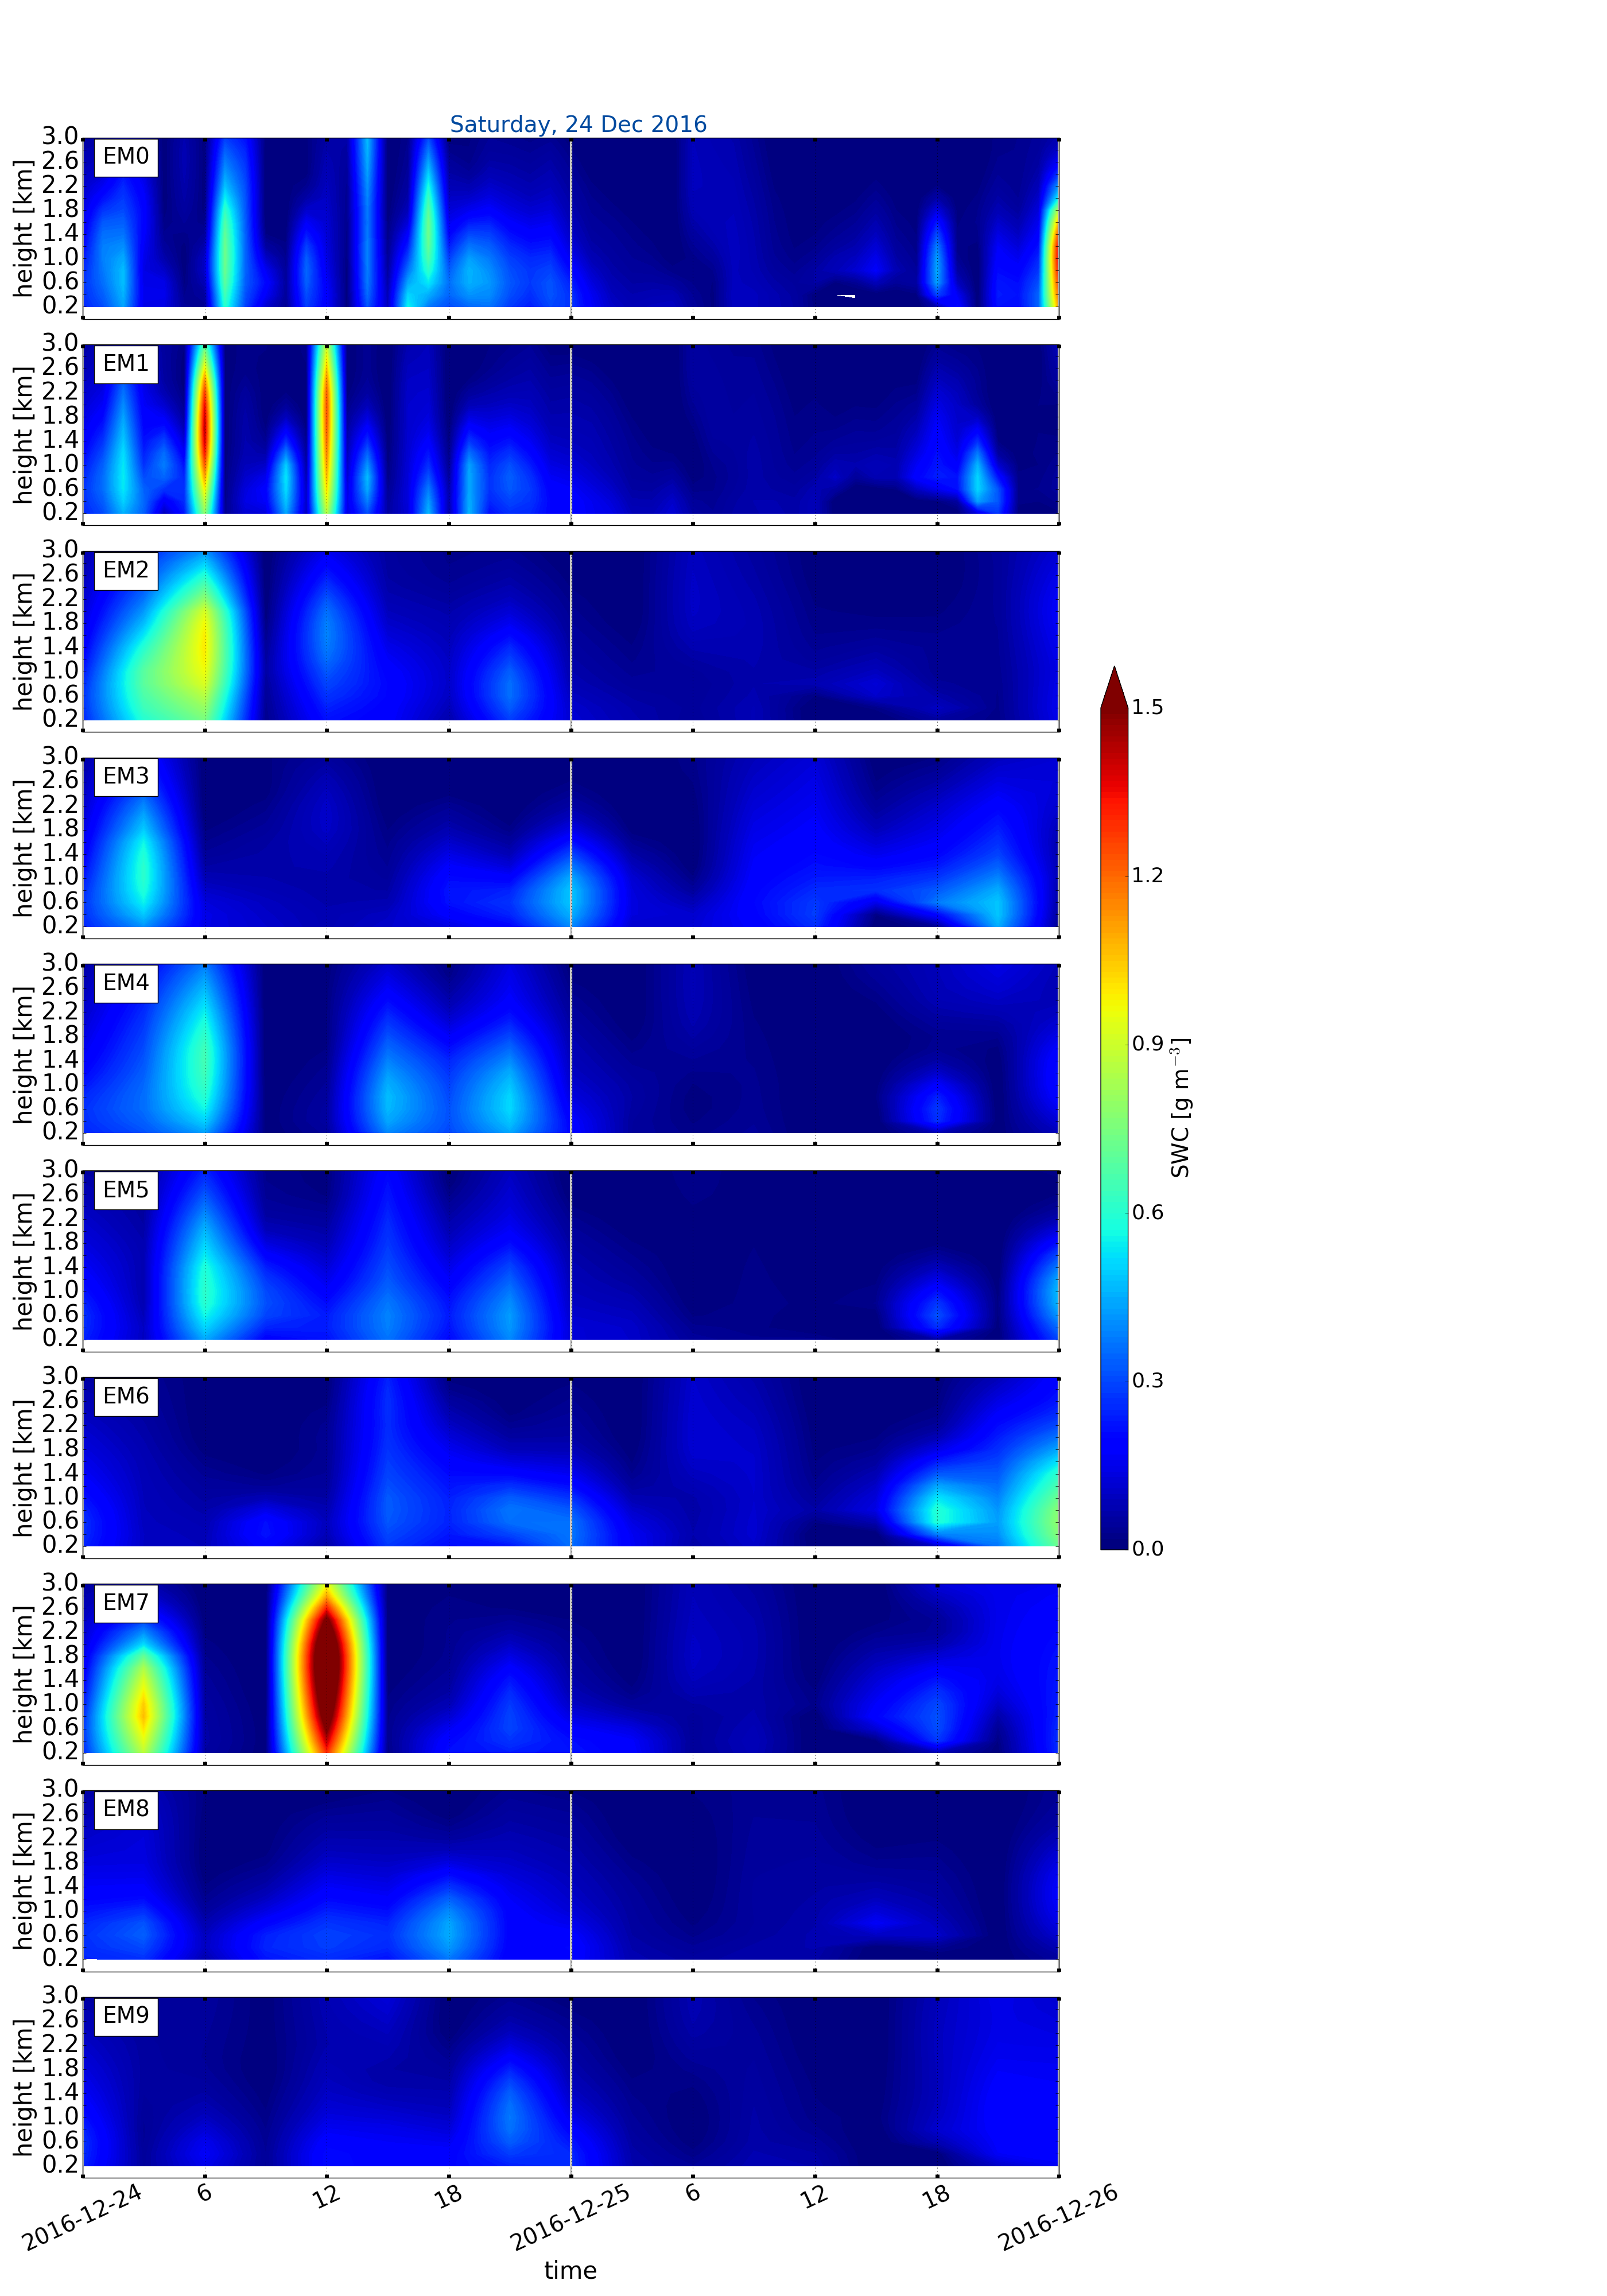
\includegraphics[trim={0cm 0cm 18.3cm 5.1cm},clip,width=0.8\textwidth]{./fig_09EM/20161224}
	\caption{SWC of all ensemble members initialised Saturday, \SI{24}{\dec} at 0\SI{0}{\UTC} forecast for \SI{48}{\hour}.}\label{fig:EM09_24}
\end{figure}
%%%%%%%%%%%%%%%%%%%%%%%%%%%%%%%%%%%%%%%%%%%%%%%%%%%%%%%%%%%%%%%%%%%%%%%%%%
\textcolor{red}{DISCUSSION! Bring all into relation and include the verification plots}


%%%%%%%%%%%%%%%%%%%%%%%%%%%%%%%%%%%%%%%%%%%%%%%%%%%%%%%%%%%%%%%%%%%%%%%%%
%%%%%%%%% 25122016 %%%%%%%%%%%%%%
 
%%%%%%%%%%%%%%%%%%%%%
% !TeX spellcheck = en_GB
\section{Saturday, \SI{25}{\dec}}\label{sec:2512}

%%% short info on Saturdays general weather


%%%%%%%%%%%%%%%%%%%%%%%%%%%%%%%%%%%%%%%%%%%%%%%%%%%%%%%%%%%%%%%%%%%%%%%%%%
%%%%%%%%% surface obs %%%%%%%%%%%%%%
\subsection{Surface accumulation}
% text 

%%% image surface MEPS boxplot %%%%%%%%%%%%%%%%%%%%%%%%%%%%%%%%%%%%%
\begin{figure}[t]
	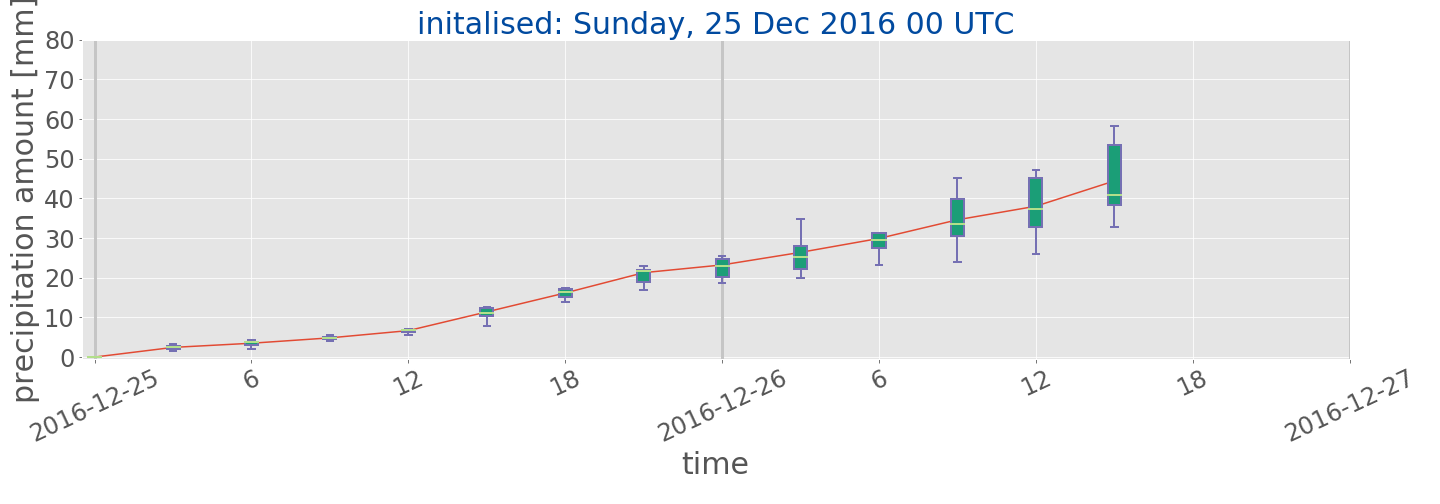
\includegraphics[width=\textwidth]{./fig_boxplot_sfc/20161225_0}
	\caption{Box-whisker-plot of the ten ensemble members of MEPS. Red line indicating the ensemble mean, lower and upper whisker the 25th and 75th percentile, respectively. Light green shows the median of all members and the box represents the middle \SI{50}{\percent} of scores of the precipitation.}\label{fig:boxplt25}
\end{figure}
%%%%%%%%%%%%%%%%%%%%%%%%%%%%%%%%%%%%%%%%%%%%%%%%%%%%%%%%%%%%%%%%%%%%%%%%%%
% text 

%%%%%%%%%%%%%%%%%%%%%%%%%%%%%%%%%%%%%%%%%%%%%%%%%%%%%%%%%%%%%%%%%%%%%%%%%%
%%%%%%%%% vertical obs %%%%%%%%%%%%%%
\subsection{Vertical snowfall observations}\label{sec:vertEM09:2512}
% %%% image SWP %%%%%%%%%%%%%%%%%%%%%%%%%%%%%%%%%%%%%
\begin{figure}[t]
	\centering
	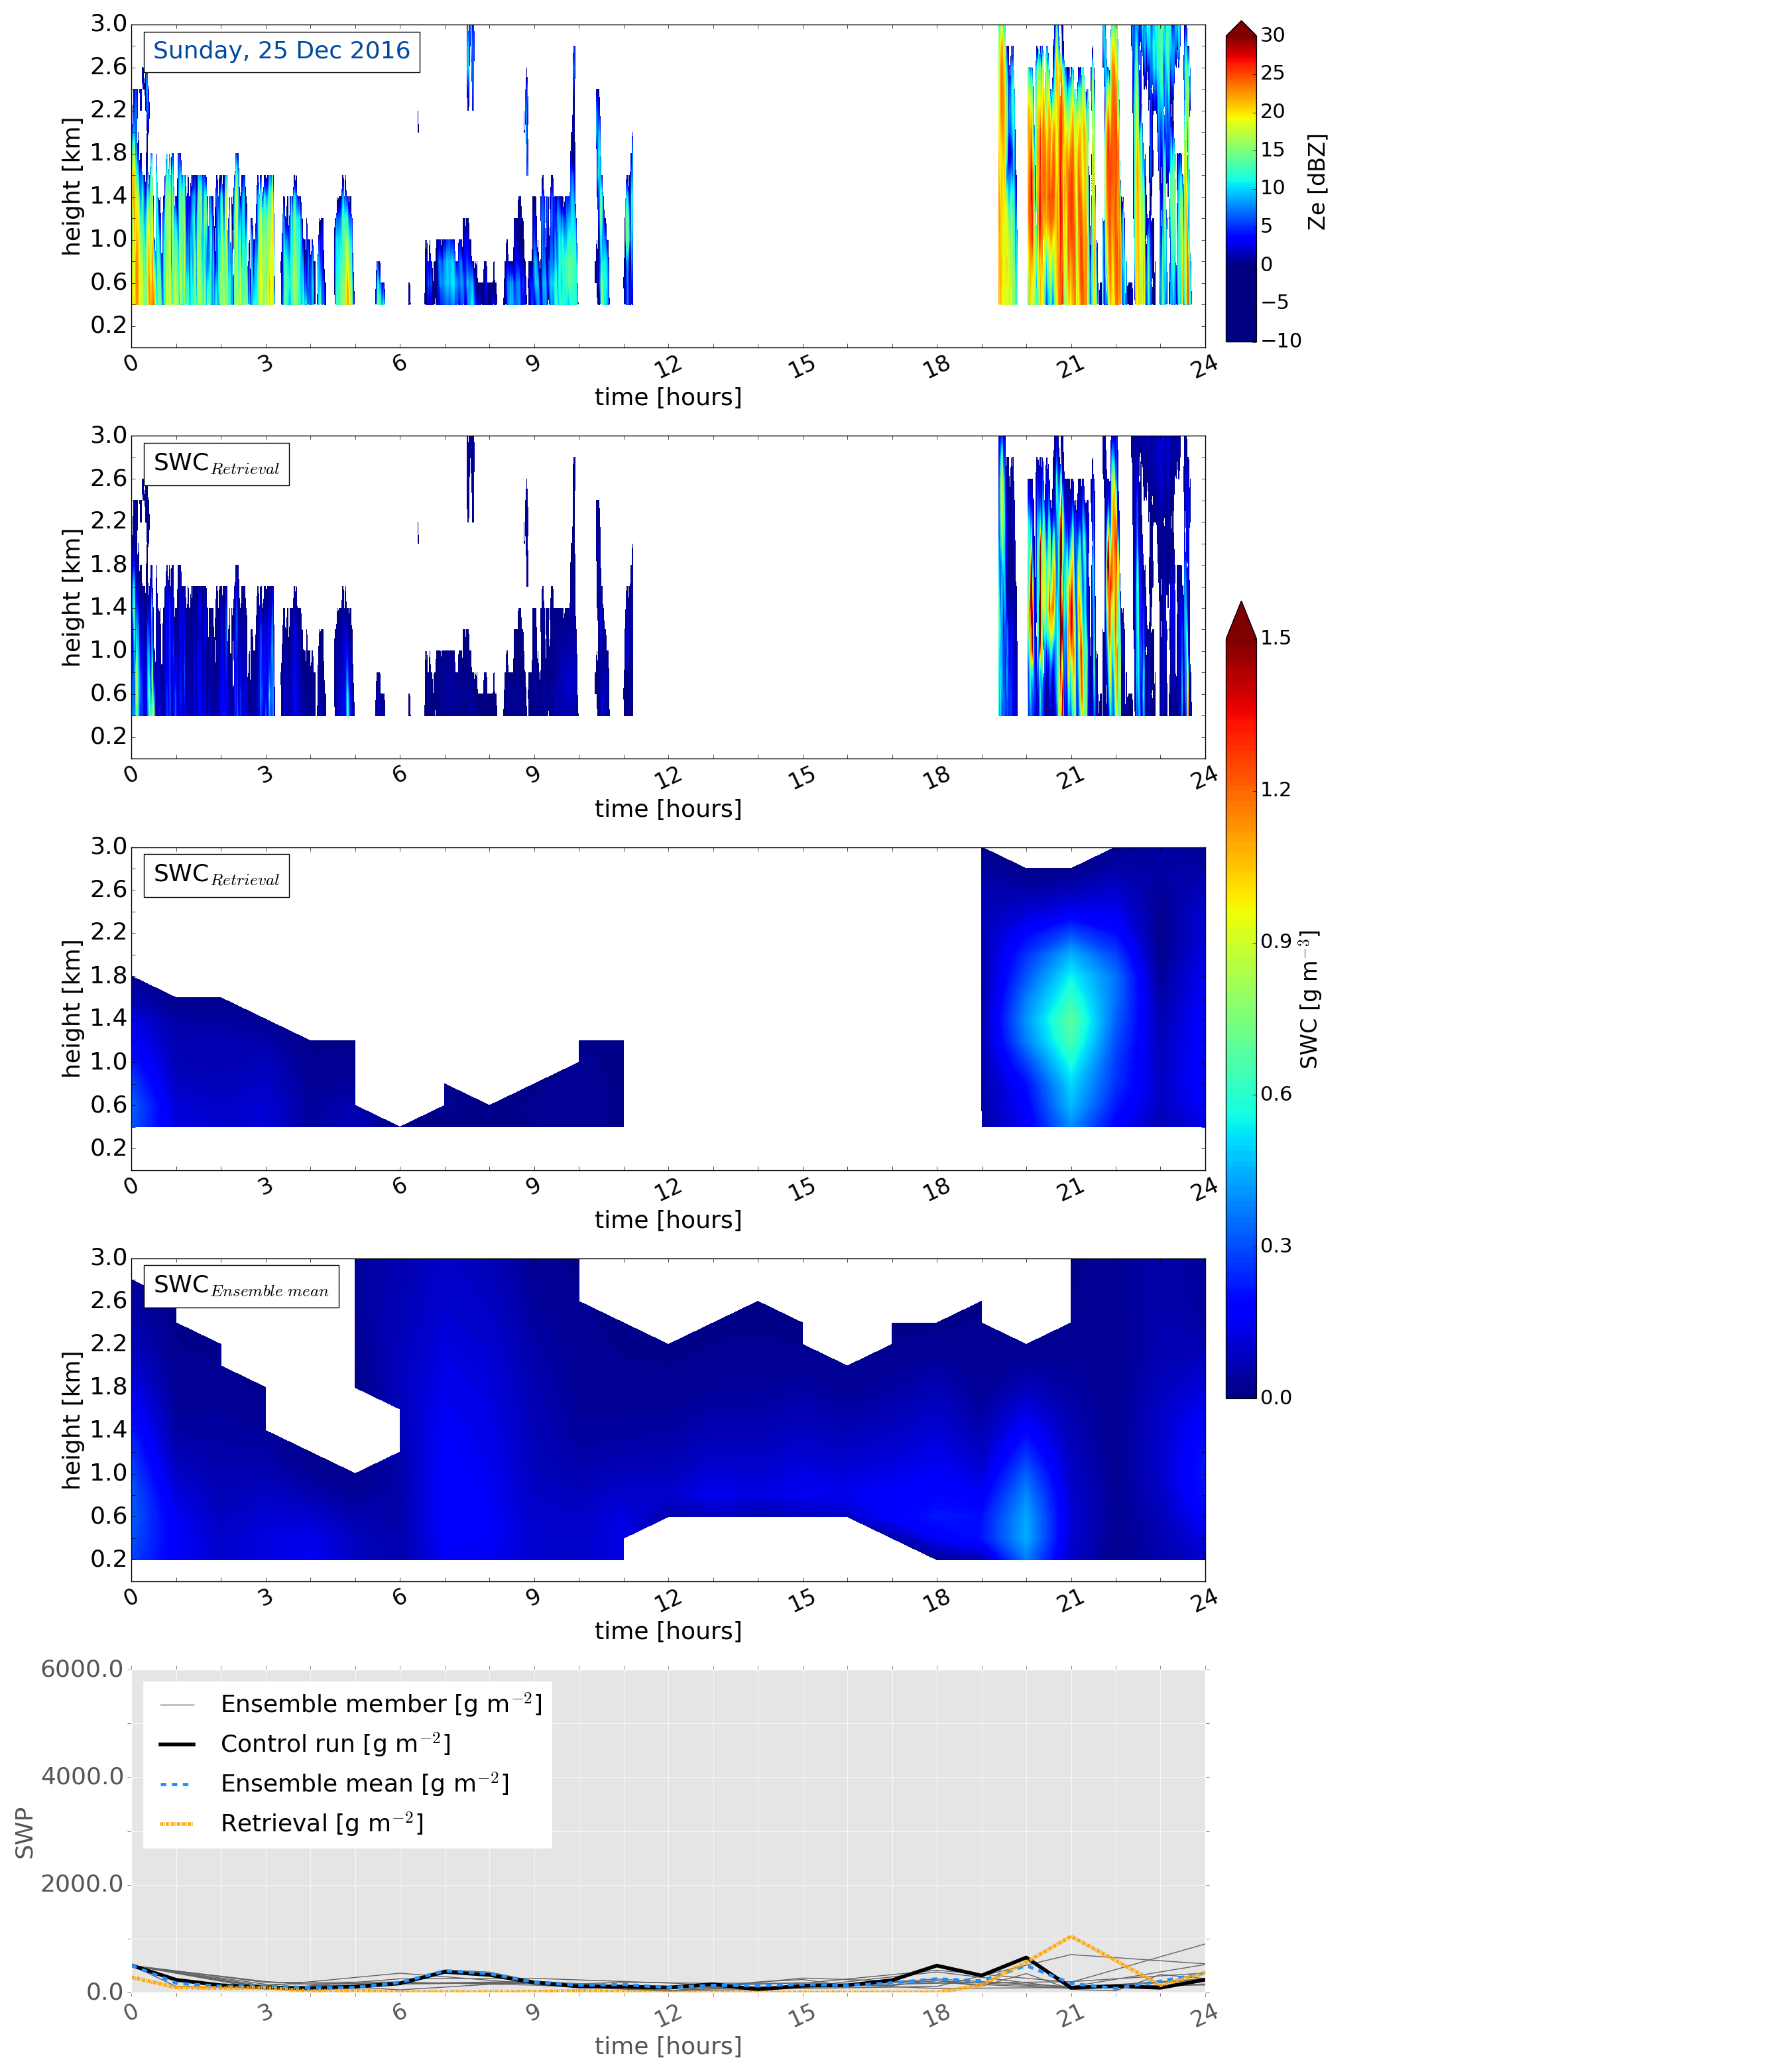
\includegraphics[trim={0.4cm .4cm 31.3cm 63.5cm},clip,width=\textwidth]{./fig_SWC/20161225}
	\caption{}\label{fig:SWP25}
\end{figure}
%%%%%%%%%%%%%%%%%%%%%%%%%%%%%%%%%%%%%%%%%%%%%%%%%%%%%%%%%%%%%%%%%%%%%%%%%%
% text
%
% %%% image ensemble member 0-9 %%%%%%%%%%%%%%%%%%%%%%%%%%%%%%%%%%%%%
\begin{figure}[t]
	\centering
	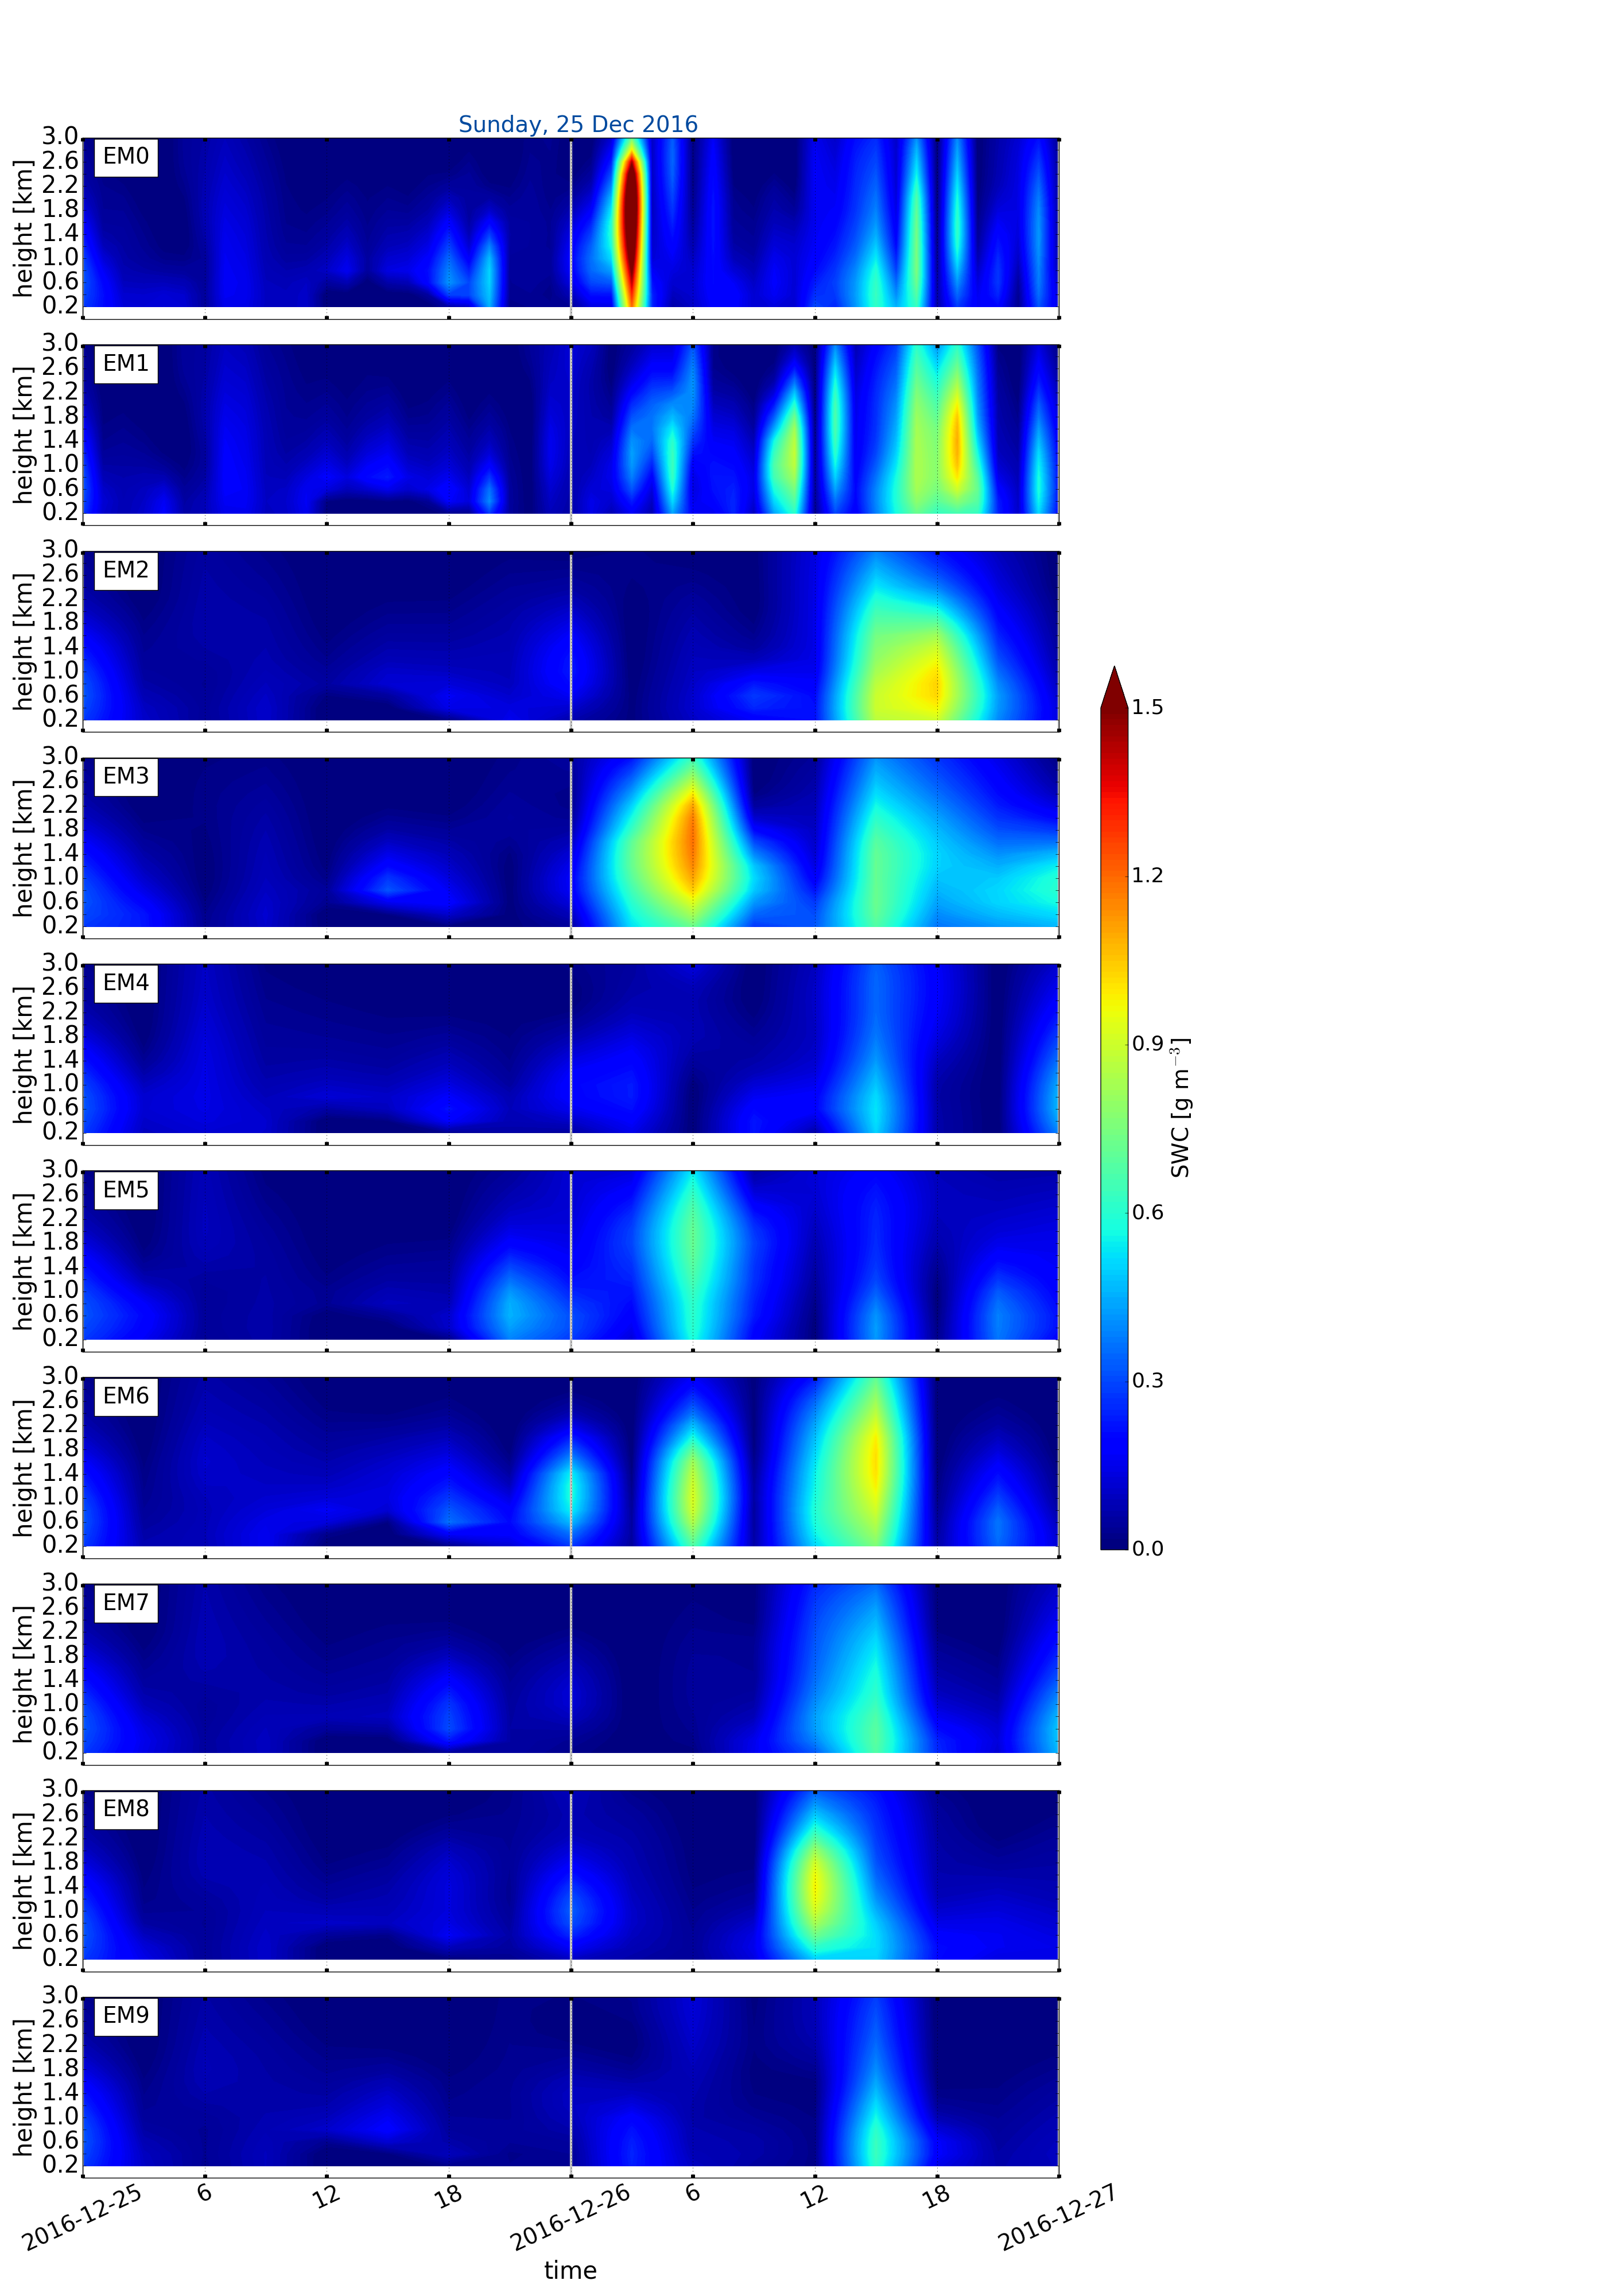
\includegraphics[trim={0cm 0cm 18.3cm 5.1cm},clip,width=0.8\textwidth]{./fig_09EM/20161225}
	\caption{SWC of all ensemble members initialised Sunday, \SI{25}{\dec} at 0\SI{0}{\UTC} forecast for \SI{48}{\hour}.}\label{fig:EM09_25}
\end{figure}
%%%%%%%%%%%%%%%%%%%%%%%%%%%%%%%%%%%%%%%%%%%%%%%%%%%%%%%%%%%%%%%%%%%%%%%%%%
\textcolor{red}{DISCUSSION! Bring all into relation and include the verification plots}



%%%%%%%%%%%%%%%%%%%%%%%%%%%%%%%%%%%%%%%%%%%%%%%%%%%%%%%%%%%%%%%%%%%%%%%%%%
%%%%%%%%% 25122016 %%%%%%%%%%%%%%
% \chapter{Summary and Conclusion}
% Even though the model might have performed well for some days it might be interesting to investigate the same results with an hourly time resolution of all ten ensemble members. Another interesting approach could also be to perturb the ensemble members and initialise them in a different way to see if the actual forecast performed best.

% % % %%%%%%%%%%%%%%%%%%%%%%%%%%%%%%%%%%%%%%%%%%%%%%%%%%%%%%%%%%%%%%%%%%%%%%%%%%

